% uWaterloo Thesis Template for LaTeX 
% Last Updated May 24, 2011 by Stephen Carr, IST Client Services
% FOR ASSISTANCE, please send mail to rt-IST-CSmathsci@ist.uwaterloo.ca

% Effective October 2006, the University of Waterloo 
% requires electronic thesis submission. See the uWaterloo thesis regulations at
% http://www.grad.uwaterloo.ca/Thesis_Regs/thesistofc.asp.

% DON'T FORGET TO ADD YOUR OWN NAME AND TITLE in the "hyperref" package
% configuration below. THIS INFORMATION GETS EMBEDDED IN THE PDF FINAL PDF DOCUMENT.
% You can view the information if you view Properties of the PDF document.

% Many faculties/departments also require one or more printed
% copies. This template attempts to satisfy both types of output. 
% It is based on the standard "book" document class which provides all necessary 
% sectioning structures and allows multi-part theses.

% DISCLAIMER
% To the best of our knowledge, this template satisfies the current uWaterloo requirements.
% However, it is your responsibility to assure that you have met all 
% requirements of the University and your particular department.
% Many thanks to the feedback from many graduates that assisted the development of this template.

% -----------------------------------------------------------------------

% By default, output is produced that is geared toward generating a PDF 
% version optimized for viewing on an electronic display, including 
% hyperlinks within the PDF.
 
% E.g. to process a thesis called "mythesis.tex" based on this template, run:

% pdflatex mythesis	-- first pass of the pdflatex processor
% bibtex mythesis	-- generates bibliography from .bib data file(s) 
% pdflatex mythesis	-- fixes cross-references, bibliographic references, etc
% pdflatex mythesis	-- fixes cross-references, bibliographic references, etc

% If you use the recommended LaTeX editor, Texmaker, you would open the mythesis.tex
% file, then click the pdflatex button. Then run BibTeX (under the Tools menu).
% Then click the pdflatex button two more times. If you have an index as well,
% you'll need to run MakeIndex from the Tools menu as well, before running pdflatex
% the last two times.

% N.B. The "pdftex" program allows graphics in the following formats to be
% included with the "\includegraphics" command: PNG, PDF, JPEG, TIFF
% Tip 1: Generate your figures and photos in the size you want them to appear
% in your thesis, rather than scaling them with \includegraphics options.
% Tip 2: Any drawings you do should be in scalable vector graphic formats:
% SVG, PNG, WMF, EPS and then converted to PNG or PDF, so they are scalable in
% the final PDF as well.
% Tip 3: Photographs should be cropped and compressed so as not to be too large.

% To create a PDF output that is optimized for double-sided printing: 
%
% 1) comment-out the \documentclass statement in the preamble below, and
% un-comment the second \documentclass line.
%
% 2) change the value assigned below to the boolean variable
% "PrintVersion" from "false" to "true".

% --------------------- Start of Document Preamble -----------------------

% Specify the document class, default style attributes, and page dimensions
% For hyperlinked PDF, suitable for viewing on a computer, use this:
\documentclass[letterpaper,12pt,titlepage,oneside,final]{book}
 
% For PDF, suitable for double-sided printing, change the PrintVersion variable below
% to "true" and use this \documentclass line instead of the one above:
%\documentclass[letterpaper,12pt,titlepage,openright,twoside,final]{book}

% Some LaTeX commands I define for my own nomenclature.
% If you have to, it's better to change nomenclature once here than in a 
% million places throughout your thesis!
\newcommand{\package}[1]{\textbf{#1}} % package names in bold text
\newcommand{\cmmd}[1]{\textbackslash\texttt{#1}} % command name in tt font 
\newcommand{\href}[1]{#1} % does nothing, but defines the command so the
    % print-optimized version will ignore \href tags (redefined by hyperref pkg).
%\newcommand{\texorpdfstring}[2]{#1} % does nothing, but defines the command
% Anything defined here may be redefined by packages added below...

\usepackage{floatpag}
%\usepackage{geometry}
%\usepackage[strict]{changepage}

% This package allows if-then-else control structures.
\usepackage{ifthen}
\newboolean{PrintVersion}
\setboolean{PrintVersion}{false} 
% CHANGE THIS VALUE TO "true" as necessary, to improve printed results for hard copies
% by overriding some options of the hyperref package below.

%\usepackage{nomencl} % For a nomenclature (optional; available from ctan.org)
\usepackage{amsmath,amssymb,amstext} % Lots of math symbols and environments
\usepackage[pdftex]{graphicx} % For including graphics N.B. pdftex graphics driver 

% Hyperlinks make it very easy to navigate an electronic document.
% In addition, this is where you should specify the thesis title
% and author as they appear in the properties of the PDF document.
% Use the "hyperref" package 
% N.B. HYPERREF MUST BE THE LAST PACKAGE LOADED; ADD ADDITIONAL PKGS ABOVE
\usepackage[pdftex,letterpaper=true,pagebackref=false]{hyperref} % with basic options
		% N.B. pagebackref=true provides links back from the References to the body text. This can cause trouble for printing.
\hypersetup{
    plainpages=false,       % needed if Roman numbers in frontpages
    pdfpagelabels=true,     % adds page number as label in Acrobat's page count
    bookmarks=true,         % show bookmarks bar?
    unicode=false,          % non-Latin characters in Acrobat’s bookmarks
    pdftoolbar=true,        % show Acrobat’s toolbar?
    pdfmenubar=true,        % show Acrobat’s menu?
    pdffitwindow=false,     % window fit to page when opened
    pdfstartview={FitH},    % fits the width of the page to the window
    pdftitle={Efficient Temporal Synopsis of Social Media Streams},    % title: CHANGE THIS TEXT!
    pdfauthor={Younes Abouelnagah},    % author: CHANGE THIS TEXT! and uncomment this line
%    pdfsubject={Subject},  % subject: CHANGE THIS TEXT! and uncomment this line
%    pdfkeywords={keyword1} {key2} {key3}, % list of keywords, and uncomment this line if desired
    pdfnewwindow=true,      % links in new window
    colorlinks=true,        % false: boxed links; true: colored links
    linkcolor=blue,         % color of internal links
    citecolor=green,        % color of links to bibliography
    filecolor=magenta,      % color of file links
    urlcolor=cyan           % color of external links
}
\ifthenelse{\boolean{PrintVersion}}{   % for improved print quality, change some hyperref options
\hypersetup{	% override some previously defined hyperref options
%    colorlinks,%
    citecolor=black,%
    filecolor=black,%
    linkcolor=black,%
    urlcolor=black}
}{} % end of ifthenelse (no else)

% Setting up the page margins...
% uWaterloo thesis requirements specify a minimum of 1 inch (72pt) margin at the
% top, bottom, and outside page edges and a 1.125 in. (81pt) gutter
% margin (on binding side). While this is not an issue for electronic
% viewing, a PDF may be printed, and so we have the same page layout for
% both printed and electronic versions, we leave the gutter margin in.
% Set margins to minimum permitted by uWaterloo thesis regulations:
\setlength{\marginparwidth}{0pt} % width of margin notes
% N.B. If margin notes are used, you must adjust \textwidth, \marginparwidth
% and \marginparsep so that the space left between the margin notes and page
% edge is less than 15 mm (0.6 in.)
\setlength{\marginparsep}{0pt} % width of space between body text and margin notes
\setlength{\evensidemargin}{0.125in} % Adds 1/8 in. to binding side of all 
% even-numbered pages when the "twoside" printing option is selected
\setlength{\oddsidemargin}{0.125in} % Adds 1/8 in. to the left of all pages
% when "oneside" printing is selected, and to the left of all odd-numbered
% pages when "twoside" printing is selected
\setlength{\textwidth}{6.375in} % assuming US letter paper (8.5 in. x 11 in.) and 
% side margins as above
\raggedbottom

% The following statement specifies the amount of space between
% paragraphs. Other reasonable specifications are \bigskipamount and \smallskipamount.
\setlength{\parskip}{\medskipamount}

% The following statement controls the line spacing.  The default
% spacing corresponds to good typographic conventions and only slight
% changes (e.g., perhaps "1.2"), if any, should be made.
\renewcommand{\baselinestretch}{1.2} % this is the default line space setting

% By default, each chapter will start on a recto (right-hand side)
% page.  We also force each section of the front pages to start on 
% a recto page by inserting \cleardoublepage commands.
% In many cases, this will require that the verso page be
% blank and, while it should be counted, a page number should not be
% printed.  The following statements ensure a page number is not
% printed on an otherwise blank verso page.
\let\origdoublepage\cleardoublepage
\newcommand{\clearemptydoublepage}{%
  \clearpage{\pagestyle{empty}\origdoublepage}}
\let\cleardoublepage\clearemptydoublepage

%======================================================================
%   L O G I C A L    D O C U M E N T -- the content of your thesis
%======================================================================

\usepackage[normalem]{ulem}

\usepackage{pdflscape}
\usepackage{mathtools}

\usepackage{algorithm2e}



\usepackage{multirow}

\begin{document}

% For a large document, it is a good idea to divide your thesis
% into several files, each one containing one chapter.
% To illustrate this idea, the "front pages" (i.e., title page,
% declaration, borrowers' page, abstract, acknowledgements,
% dedication, table of contents, list of tables, list of figures,
% nomenclature) are contained within the file "uw-ethesis-frontpgs.tex" which is
% included into the document by the following statement.
%----------------------------------------------------------------------
% FRONT MATERIAL
%----------------------------------------------------------------------
% T I T L E   P A G E
% -------------------
% Last updated May 24, 2011, by Stephen Carr, IST-Client Services
% The title page is counted as page `i' but we need to suppress the
% page number.  We also don't want any headers or footers.
\pagestyle{empty}
\pagenumbering{roman}

% The contents of the title page are specified in the "titlepage"
% environment.
\begin{titlepage}
        \begin{center}
        \vspace*{1.0cm}

        \Huge
        {\bf Efficient Temporal Synopsis of Social Media Streams }

        \vspace*{1.0cm}

        \normalsize
        by \\

        \vspace*{1.0cm}

        \Large
       Younes Abouelnagah\\

        \vspace*{3.0cm}

        \normalsize
        A thesis \\
        presented to the University of Waterloo \\ 
        in fulfillment of the \\
        thesis requirement for the degree of \\
        Master of Math \\
        in \\
        Computer Science \\

        \vspace*{2.0cm}

        Waterloo, Ontario, Canada, 2013 \\

        \vspace*{1.0cm}

        \copyright\ Younes Abouelnagah 2013 \\
        \end{center}
\end{titlepage}

% The rest of the front pages should contain no headers and be numbered using Roman numerals starting with `ii'
\pagestyle{plain}
\setcounter{page}{2}

\cleardoublepage % Ends the current page and causes all figures and tables that have so far appeared in the input to be printed.
% In a two-sided printing style, it also makes the next page a right-hand (odd-numbered) page, producing a blank page if necessary.
 


% D E C L A R A T I O N   P A G E
% -------------------------------
  % The following is the sample Delaration Page as provided by the GSO
  % December 13th, 2006.  It is designed for an electronic thesis.
  \noindent
I hereby declare that I am the sole author of this thesis. This is a true copy of the thesis, including any required final revisions, as accepted by my examiners.

  \bigskip
  
  \noindent
I understand that my thesis may be made electronically available to the public.

\cleardoublepage
%\newpage

% A B S T R A C T
% ---------------

\begin{center}\textbf{Abstract}\end{center}
Search and summarization of streaming social media, such as Twitter, requires the ongoing analysis of large volumes of data with dynamically changing characteristics.  Tweets are short and repetitious~--~lacking context and structure~--~making it difficult to generate a coherent synopsis of events within a given time period.  Although some established algorithms for frequent itemset analysis might provide an efficient foundation for synopsis generation, the unmodified application of standard methods produces a complex mass of rules, dominated by common language constructs and many trivial variations on topically related results.  Moreover, these results are not necessarily specific to events within the time period of interest.  To address these problems, we build upon the Linear time Closed itemset Mining (LCM) algorithm, which is particularly suited to the large and sparse vocabulary of tweets.  LCM generates only closed itemsets, providing an immediate reduction in the number of trivial results.  To reduce the impact of function words and common language constructs, we apply a filtering step that preserves these terms only when they may form part of a relevant collocation.  To further reduce trivial results, we propose a novel strengthening of the closure condition of LCM to retain only those results that exceed a threshold of distinctiveness.  Finally, we perform temporal ranking, based on information gain, to identify results that are particularly relevant to the time period of interest.  We evaluate our work over a collection of tweets gathered in late 2012, exploring the efficiency and filtering characteristic of each processing step, both individually and collectively.  Based on our experience, the resulting synopses from various time periods provide understandable and meaningful pictures of events within those periods, with potential application to tasks such as temporal summarization and query expansion for search.

\cleardoublepage
%\newpage

% A C K N O W L E D G E M E N T S
% -------------------------------

\begin{center}\textbf{Acknowledgements}\end{center}
I would like to thank all the people who made this possible.
First and foremost, my supervisor Charles Clarke for giving me
the opportunity to join such a great university,
and for providing a very encouraging learning environment.
Second, my family for making my life worry free, 
specially my wife Nada who was very patient 
during all the time I was away from her.
Last but not least, my colleagues in this journey of
development with whom I worked and grew.
 

\cleardoublepage
%\newpage

% D E D I C A T I O N
% -------------------

\begin{center}\textbf{Dedication}\end{center}

This is dedicated to the my people struggling for freedom and democracy in the Arab world, while I comfortably study in beautiful Canada.
\cleardoublepage
%\newpage

% T A B L E   O F   C O N T E N T S
% ---------------------------------
\renewcommand\contentsname{Table of Contents}
\tableofcontents
\cleardoublepage
\phantomsection
%\newpage

% L I S T   O F   T A B L E S
% ---------------------------
\addcontentsline{toc}{chapter}{List of Tables}
\listoftables
\cleardoublepage
\phantomsection		% allows hyperref to link to the correct page
%\newpage

% L I S T   O F   F I G U R E S
% -----------------------------
\addcontentsline{toc}{chapter}{List of Figures}
\listoffigures
\cleardoublepage
\phantomsection		% allows hyperref to link to the correct page
%\newpage

% L I S T   O F   S Y M B O L S
% -----------------------------
% To include a Nomenclature section
% \addcontentsline{toc}{chapter}{\textbf{Nomenclature}}
% \renewcommand{\nomname}{Nomenclature}
% \printglossary
% \cleardoublepage
% \phantomsection % allows hyperref to link to the correct page
% \newpage

% Change page numbering back to Arabic numerals
\pagenumbering{arabic}

 

%----------------------------------------------------------------------
% MAIN BODY
%----------------------------------------------------------------------
% Because this is a short document, and to reduce the number of files
% needed for this template, the chapters are not separate
% documents as suggested above, but you get the idea. If they were
% separate documents, they would each start with the \chapter command, i.e, 
% do not contain \documentclass or \begin{document} and \end{document} commands.
%======================================================================
\chapter{Introduction}
%======================================================================
%\category{H.4}{Information Systems Applications}{Miscellaneous}
%A category including the fourth, optional field follows...
%\category{D.2.8}{Software Engineering}{Metrics}[complexity measures, performance measures]

%\terms{Theory}

%\keywords{ACM proceedings, \LaTeX, text tagging}
\section{Social Media Text}
Text posted on social media outlets, such as Twitter, is a good and timely source of information
about real world events~\cite{ritter2012open}. 
It also includes posts about other topics attracting the collective attention of user communities, 
such as Internet memes or large scale discussions~\cite{naaman2011hip}.
Nevertheless, the collective stream from all users is overwhelmed by personal
updates and non-informative chatter~\cite{java2007we,hurlock2011searching}. 
Furthermore, the attention span given to the majority of topics is quite short~\cite{kwak2010twitter}.
Finding posts about topics of interest in a timely fashion
requires an efficient mining algorithm.

To realize the benefits of social media in giving a voice to ordinary people,
the algorithm should mine the content of posts 
without explicitly assigning weights based on popularity of users. % to posts made by ``influencers''.
However, the nature of text in social media poses a challenge when applying
traditional text mining algorithms. 
Text in social media is usually short, undermining the effectiveness of within document frequency counting.
It lacks context, since posts are standalone and most platforms do not allow explicit linkage.
It also lacks structure and other useful formatting cues. 
One type of mining algorithms that can be applied to such data is frequent itemset mining.

\section{Frequent Itemset Mining}

Frequent itemset mining algorithms count the number of times each
combination of ``items'' appear together. 
This is called the support of the itemset.
An itemset is considered frequent if its support is above a threshold.
When mining textual data, 
an item is usually taken to be a unigram. %can be a unigram or 
A set of items are considered to be
appearing together if they appear within the same document
or paragraph. The frequent itemset mining family of algorithms is fast and efficient,
however it is not readily suited for application on text. 
Following are a number of challenges faced when applying 
frequent itemset mining to textual data. In this thesis we address those problems, adapting frequent itemset mining to
social media text without degrading its efficiency:

\begin{enumerate}
\item
The number of itemsets mined grows with the number of
distinct items~--~which is particularly high in the text domain.
In social media, the problem is complicated by the continuous creation 
of new tokens~\cite{lin2012study}, in the form of hashtags or usernames,
and due to shortening of words because of the length limit of some platforms.

\item
The number of frequent itemsets is generally high.
Frequent itemset mining was originally proposed as a preliminary stage for
association rules mining, which sifts through the numerous itemsets and
produces a smaller number of rules associating combinations of items with each other.
To reduce the number of itemsets, they may be limited by setting a high
support threshold. This is not possible in text mining because
the frequency of most items is low, and only a few items have high frequencies;
that is, frequencies of items follow a long-tailed Zipfean distribution.

\item
Function words are among the few items having high frequencies. 
This leads to mining a large number of itemsets which are uninformative language constructs.
Even if a maximum frequency threshold is set, incurring the risk that we
will filter out important itemsets, many  non-English constructs will be
mined because the proportion of posts in English is much higher than
other languages. 
Notice that we do not remove function words 
%for reasons that will be detailed later.
so that we allow mining itemsets made up solely of function words, 
and to make the mining results easier to understand at the user level.

\item
%Finally, t
There is considerable redundancy in frequent
itemsets caused by trivial differences in the language used.
\end{enumerate}


\section{Motivation and Contributions}
Frequent itemset mining is suitable to the dynamic nature of social media streams.
It does not require prior knowledge of the distribution of items,
nor does it require selecting a few items to monitor 
or a number of topics to mine. %preset
It is fast, efficient and scalable. 
It is also robust against data sparsity, 
and can actually exploit this sparsity for faster computation.
Unlike trending topics\footnote{\url{http://blog.twitter.com/2010/12/to-trend-or-not-to-trend.html}}
\cite{mathioudakis2010twittermonitor}, the results of frequent itemset
mining include itemsets that have high frequency because of sustained interest,
as well as a spike of interest.

The mined itemsets provide the vocabulary associated with events and can be
used as a preliminary step for search and summarization.
For example, the collection of mining results from different epochs of time
can be used for temporal 
query expansion and document expansion~\cite{choi2012temporal, efron2012improving}.
Expansion methods can be specially developed  
%to build on the mining results,
based on the mining results,
but it is also possible to use existing methods.
The results from each epoch can be treated as a document,
and relevant ``documents'' can be used to
%facilitating the creation of 
create
a \emph{temporal profile}~\cite{jones2007temporal} 
of the query or document being expanded.
For summarization, frequent itemsets can provide a good foundation for summary
creation.
While the frequent itemsets themselves are not summaries, since they lack
qualitative properties such as coherence and cohesion, the results are
understandable at the user level.
As we shall see in later examples, the top ranked itemsets cover a variety
of open topics, and within one topic different opinions are reported as
separate contrastive itemsets.

Previous work has proposed methods tailored for the use of frequent itemsets (patterns) to improve search performance.  
Itemsets provide better semantics than keywords, and have better statistical properties than phrases~\cite{wu2006deploying}.
By using carefully selected itemsets and filtering out ``meaningless'' ones, 
\emph{pattern-based} approaches achieve better performance
than keyword-based approaches~\cite{wu2004automatic}. % and phrase based approaches
However, the choice of ``interesting'' or ``informative'' itemsets 
and filtering out ``meaningless'' ones remains an area of active research.
In Li et al.~\cite{li2010mining} itemsets are mined from
paragraphs of newswire text, and are used to determine term weights for query
expansion.
Improvements in performance have been achieved by using itemsets taken from
a training set of related documents, as well as ones from unrelated documents.
In a more recent work, an unsupervised version that relies on co-occurrence of 
itemsets within the same paragraph has been proposed~\cite{albathan2012using}.

In this thesis, we propose efficient methods for filtering out non-informative frequent itemsets,
reducing redundancy in the mining results, and ranking the selection according to temporal novelty.
Our methods exploit the dynamics of social media and make use of the collaborative filtering
that users naturally undergo on social media, 
by sharing interesting posts and participating in conversations.
Our main contributions are as follows:
\begin{itemize}
\item We propose the use of variable length term N-grams as items to avoid mining uninformative language constructs as itemsets. 
\item We propose a condition for selecting informative itemsets, and a clustering scheme for reducing redundancy in the mining results.
\item We propose a formula for ranking itemsets according to temporal novelty.
\end{itemize}
The effectiveness of our methods is shown quantitatively, 
in terms of the reduction in the number of itemsets at each processing step. 
The quality of the final outcome is verified by showing mining results from various time periods.

\section{Thesis Outline}

The next two chapters provide necessary background.
We start by discussing related work in chapter \ref{sec:related},
then we explain the algorithm on which we build
our work in chapter~\ref{sec:socmine}.
In chapter~\ref{sec:socmine}, 
we also introduce the dataset we use, 
and the data prepocessing necessary for 
running a frequent itemset mining algorithm
on social media text effectively.
The most important contribution in this chapter
is a simple method for flattening the Zipfean distribution
of items, and thus reduce the number of itemsets 
%that are language constructs.
made up of function words.
Chapter~\ref{sec:strong} presents
our main contributions for creating temporal synopses 
from frequent itemsets. % mining to social media text.
We present in it our proposed condition for selecting itemsets,
the clustering scheme for grouping together itemsets
according to their topic,
and a ranking formula that is suitable
for ranking clusters according to  
temporal novelty (based on the
collective Infomration Gain of itemsets in them).
In chapter~\ref{sec:empirical}, we empirically 
evaluate the efficiency and the effectiveness 
of our proposed methods. 
Finally, we conclude our presentation and
suggest future directions in chapter~\ref{sec:concfut}.

\section{Terminology and Notation}
Classically, frequent itemset mining is applied to a \emph{database} of
\emph{transactions} made at a retail store.
This terminology is suitable for market basket data and we retain it out of
convention, even though we are mining text where the terms ``corpus'' and
``document'' are normally used.
Because of the dynamic nature of social media, rather than giving the whole
database as input to mining algorithms, the input is an \emph{epoch} of data;
data with timestamps within a certain period of time.
The epoch's \emph{span} is the length of this period in hours,
and the \emph{volume velocity} at this epoch is the number of transactions in the epoch
divided by its \emph{span}.

We now introduce the notation used in this thesis:
\begin{itemize}
\item $W = \{w_1,w_2,\ldots, w_n\}$: The set of all items occurring within the epoch of data being mined. Items can be terms or term N-grams in this thesis. % This is the \emph{vocabulary} in Information Retrieval.
\item $t_a = \{w_{a_1},\ldots, w_{a_m}\}$: A transaction made up of a set of items. Each transaction has a sequential id derived from its timestamp (denoted by the subscript letter).
\item $E^{span} = \langle t_a, t_b, \ldots, t_v\rangle$: An epoch of data of a certain span, such as an hour, made up of the sequence of the transactions created within this hour.
\item $s \subset W$: An itemset; any possible combination of items. 
\item $T_s = \{t: t \in E \, and \, s \subseteq t\}$: All transactions containing itemset s. We refer to it as the itemset's postings list, as is common in the Information Retrieval (IR) literature.
\end{itemize}




%=====================================




\chapter{Background and Related Work}
\label{sec:related}

\section{Frequent Itemset Mining}
Frequent itemset mining comprises a large body of work that goes back to the
early 1990s~\cite{agrawal1993mining}. 
%A variety of algorithms have been proposed, and they work in totally different ways. 
We categorize frequent itemset mining algorithms into
1) algorithms that operate in the item space, 
2) algorithms that operate in the transaction space, 
and 3) algorithms that operate in the solution space. 
While a comprehensive survey is beyond the scope of this thesis, 
we discuss at least one representative from each category of algorithms.

\subsection{The Apriori Algorithm}
%Frequent itemset mining was proposed 
% was 
%The Apriori algorithm is the first efficient algorithm for frequent itemset mining~\cite{agrawal1994fast}, 
%proposed by Agrawal et al. as part of the solution to the problem of association rules mining. 
%It's goal was finding itemsets that can be broken into a precedent and an antecedent
Agrawal et al.~\cite{agrawal1994fast} proposed the Apriori algorithm 
as part of the first efficient solution to the problem of association rules mining~\cite{agrawal1993mining}.
In the domain of market basked data, 
an association rule is an implication that an item is likely to be purchased
in the same transaction with a certain set of items.
Association rules are mined by finding itemsets that co-occur together frequently, 
then producing a rule with each individual item as a consequent to the purchase of the rest of the itemset.
The Apriori algorithm finds frequent itemsets of increasing lengthes iteratively.
It starts by counting frequencies of individual items (itemsets of length 1). 
Then it iteratively increases the length of itemsets.
At each iteration, it generates candidate itemsets of length $k$ ($k$-itemsets) 
by merging frequent itemsets of length ($k$-1) (($k$-1)-itemsets) 
that differ in only 1 item, 
usually the last item given a certain total ordering of items.
By using only the frequent  ($k$-1)-itemsets for generating candidate $k$-itemsets,
many possible $k$-itemsets are implicitly pruned, 
based on the anti-monotonicity between itemsets' support and length:
all subsets of a frequent itemset must be frequent. 
However, each candidate has to be explicitly checked to verify that it does not
have any infrequent subsets.

Apriori and algorithms based on it suffer performance degradation 
and  large increases in memory requirement
when the number of distinct items is high.
These limitations are caused by the candidate generation bottleneck.
A large number of candidates can be generated,
especially in early iterations of the algorithm.
Consider, for example, the generation of candidate 2-itemsets from a database.
This generation requires producing all unordered pairs of 1-itemsets (terms),
after pruning out rare ones with frequency less than the support threshold.
In many domains, including text mining, the number of frequent 1-itemsets is
large enough to prohibit generating a number of candidates in the order of this
number squared.
In text mining, a rather low support threshold has to be used, because the
frequency of terms follow a long-tailed Zipfean distribution.

The Apriori based family of algorithms operates in the item space 
in the sense that an itemset can be expanded by any item regardless
of whether there is any support for the combination. 
%Its efficiency comes from using the current solution to prune out
Operating in the transaction space avoids this blind enumeration
of unsupported candidates, and the subsequent DB scan required 
to count the support of those candidates. 
This involves the creation of a succinct representation of the DB
that is well suited for itemset mining.

\subsection{The FP-Growth Algorithm}
The first algorithm proposed based on the idea of avoiding candidate
generation was FP-Growth~\cite{han2000mining}.
%and traversing a data structure instead
The database is represented as a frequency ordered prefix tree called the FP-tree.
Items with low support are removed, so that 
any node in the FP-tree is necessarily an item with enough support.
An FP-tree imposes the invariant that within each branch the frequency is
non-increasing from the root down to the leaves. 
This increases the chance of finding common prefixes.
%Nodes that are
An FP-tree also contains links between nodes representing the same item.
Those links are used to create the \emph{conditional} FP-tree for an item,
%which is the FP-tree where this item is the root.
which is the FP-tree made only from branches containing this item, 
excluding any items with lower frequency.
The algorithm proceeds by iterating over items in increasing order 
of frequency. 
%For each item, (1) it is output as an itemset,
%and (2) its \emph{conditional} FP-Tree is created and recursively mined. 
Each item is first output as an itemset,
and then its \emph{conditional} FP-Tree is created and recursively mined. 
At each recursive call, the current item is appended to a growing prefix,
which is prepended to all itemsets mined from the conditional FP-tree.
Figure \ref{fig:fpgrowth}, borrowed from Han et. al~\cite{han2004mining}, shows a few steps in the FP-Growth algorithm.
%during the call.

The navigation of a representation of the database 
avoids the candidate generation bottleneck,
by directly deriving itemsets from the transaction space.
However,
the creation of such representation is a bottleneck itself. 
Building conditional pattern bases and sub-FP-trees becomes time and space consuming as the recursion goes deep and the number of patterns becomes large~\cite{wang2002top}.
%Many alternate representations as well as enhancements to the original FP-Growth
%algorithm were proposed~\cite{cats.....}, however they still operate in the same way.

\begin{figure}%[h]
\centering
\scalebox{0.3}{
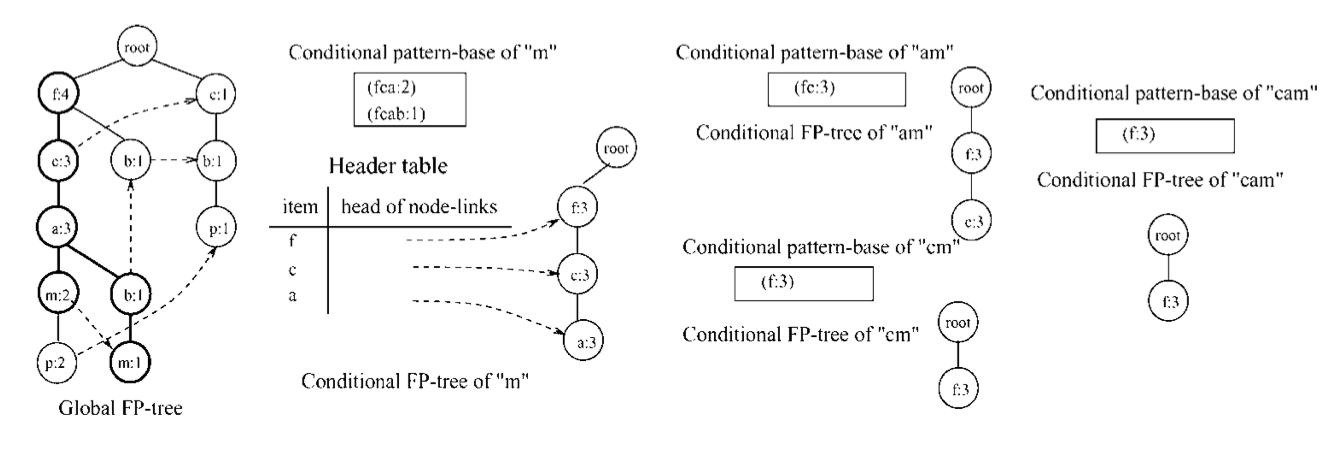
\includegraphics{fp-growth_han-2004.png}
}

\caption{A few steps in the FP-Growth algorithm as depicted by Han et al.~\cite{han2004mining}}
\label{fig:fpgrowth}
\end{figure}

\subsection{Solution Space Algorithms}
\label{sec:sol_space_algs}
The last category of frequent itemset mining algorithms comprises algorithms that operate in the solution space. 
It can be argued that algorithms that traverse a representation of the DB are operating in the solution space rather than the transaction space~--~given that they avoid generating candidates with low support. 
However, in our categorization we focus on the logic behind how itemsets are generated or pruned rather than the data structure used to generate them.
After all, any algorithm must calculate the support of itemsets, 
and this requires the algorithm to either maintain a representation of the DB or scan the transactions. 
Algorithms that operate in the solution space prune itemsets that do not possess certain properties. 
The limited number of itemsets that possess the desired property are sufficient to deduce the rest of the solution (other frequent itemsets and their support information).
The reduction in the number of itemsets mined improves the performance of such algorithms, 
even if they rely on candidate generation to enumerate possible itemsets before checking for the desired property.
It is not always necessary to produce the full solution 
since the properties usually filter out only redundant itemsets, 
and in many cases the elect itemsets can be used directly.

%The elect itemsets can be used directly, since the properties usually filter out 
%%to creates a concise representation of the solution 
%%by removing redundancy.
%redundant itemsets only.

The \emph{closure property}~\cite{pasquier1999discovering,pasquier1999efficient,zaki2002charm} prunes an itemset
if it has the same support as its supersets. 
It is easy to see that all itemsets and their support can be derived from the set of \emph{closed} itemsets. 
A formal proof is given by Pasquier et al.~\cite{pasquier1999discovering}.
The smallest itemset of an equivalence class of itemsets having the same support
is called a \emph{generator}~\cite{kryszkiewicz2001concise} or a \emph{free set}~\cite{boulicaut2000approximation}. 
It is also possible to keep only the generator of each equivalence class, 
but in this case some infrequent itemsets has to be kept 
in order to be able to calculate the support of all frequent itemsets~\cite{kryszkiewicz2001concise}. 
A different selection of itemsets can be made according to the \emph{non-derivable} property~\cite{calders2002mining,calders2007non}, 
which is linked to the closed property. %former properties. 

Finding closed itemsets can be done by arranging possible itemsets into a Galois lattice, 
then traversing the lattice using the Galois connection between itemsets and transactions
in which they appear. 
Figure~\ref{fig:lattice} shows an example of a Galois lattice. 
The Galois connection is a pair of operators, one to map an itemset to transactions in which it appears, 
and another to map a set of transactions to the largest itemset that appears in all of them.
Applying the two operators in cascade grows an itemset directly to its closed superset.
More details can be found in Pasquier et al.~\cite{pasquier1999efficient} and Zaki et al.~\cite{zaki2002charm}.

\begin{figure}
\centering
\begin{tabular}{|c|p{1.7cm}|}
\hline
TID&Items\\\hline
1&A B C\\
2&B C E\\ 
3&A B C E\\
4&B E\\
5&A B C E\\
\hline
\multicolumn{2}{c}{The transaction database}\\
\multicolumn{2}{c}{}\\
\end{tabular}
\scalebox{0.5}{
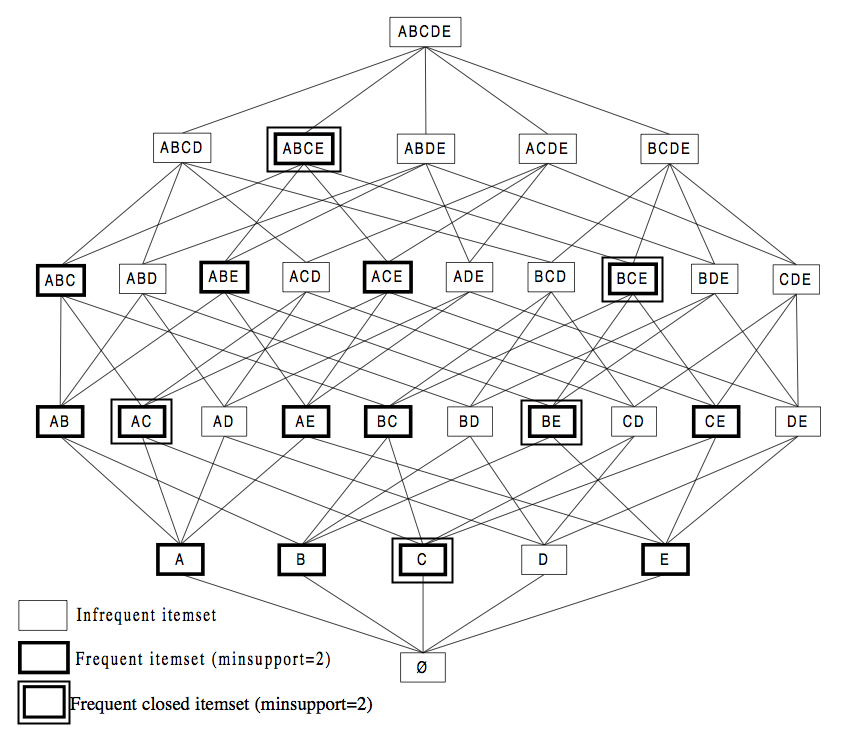
\includegraphics{galois-lattice.png}
}
\caption{Example of a Galois lattice adapted from Pasquier et al.~\cite{pasquier1999efficient}}
\label{fig:lattice}
\end{figure}

Some algorithms take advantage of the closure property to 
reduce the search space more dramatically,
such as CLOSET~\cite{pei2000closet}
and LCM~\cite{uno2004lcm}.
Our work is based on LCM (which stands for Linear-time Closed itemset Mining)~\cite{uno2004lcm}.
As a starting point for our work, we use the implementation of LCM submitted
to the workshop for Frequent Itemset Mining Implementations (FIMI) in
2004~\cite{DBLP:conf/fimi/2004}, which was the workshop's award winner. 
The LCM algorithm is robust against data sparsity, 
and has low memory requirements 
since it does not store intermediate results.
We will explain the closure property and describe LCM in detail in  section \ref{sec:lcm}. 
We proceed by discussing other areas of related work.

%-------------------------------------------------------

\section{Election of Representative or Interesting Itemsets}

The problem of having many itemsets, with redundancy and noise, can be addressed by
picking out  representative itemsets that satisfy a certain condition.
%based on the conciseness or interestingness or the selection.
The representative itemsets are not necessarily sufficient to
deduce the rest of the solution (itemsets and their support information).
In this thesis we propose a condition for selecting interesting itemsets, 
which we call
\emph{distinct} itemsets. % and  \emph{strongly closed} itemsets.
Related approaches to picking out representative itemsets are %: 
1) choosing a set that will minimize the reconstruction error of the full solution, 
and 2) limiting the number of itemsets to a user specified number.


%Most similar to the \emph{distinct} itemsets we propose in this thesis
%Choosing $\delta$-free~\cite{boulicaut2003free} or 
% $\delta$-covered~\cite{xin2005mining} itemsets are

The $\delta$-free~\cite{boulicaut2003free},  
$\delta$-covered~\cite{xin2005mining}, and 
\emph{master} itemsets~\cite{yan2005summarizing} 
are examples of conditions motivated by providing a compressed representation
of itemsets through sacrificing support information.
The $\delta$-free condition selects an itemsets if its support
is different from the support of all its subsets by at least $\delta$.
This selection of itemsets can be used to approximate the support 
of other frequent itemsets with a guarantee on the error,
but only if some infrequent itemsets are included in the selection.
The $\delta$-free condition implies setting an upper bound on the
strength of association rules that can be derived from selected itemsets.
It is suitable for compressing mining results from dense datasets,
but it is exactly the opposite of \emph{distinctiveness} condition we propose in this thesis. 


The $\delta$-covered condition is also the opposite of the \emph{distinctiveness}
condition, as it ``relaxes the closure condition to further reduce pattern
set size'' \cite{liu2012finding}. On the other hand, the \emph{distinct}  condition strengthens the closure condition.
The $\delta$-covered condition sets an upper bound on the confidence of the rule that 
an itemset implies a superset; 
if an itemset implies its superset with confidence greater than $\delta$, 
then it is considered to be covered by the superset and can be pruned.
On the other hand, the \emph{distinct} condition
%selects only itemsets that are implied by a subset with high confidence.
sets a lower bound on the confidence of a derived association rule.
Nevertheless, the clustering scheme Xin et al.~\cite{xin2005mining} propose
($\delta$-clusters) is similar to the \emph{strongly closed
itemset} clusters proposed in this thesis. 
The efficient version of the clustering algorithm, RPLocal, % proposed by Xin et al.
limits the search space for clustering candidates using a similar reasoning to 
the reasoning used in our algorithm~--~exploiting the sequence in which frequent itemsets are found.
The main difference between $\delta$-clusters and \emph{strongly closed itemset} clusters
is that $\delta$-clusters are soft clusters, while \emph{strongly closed itemset} clusters
are hard clusters. 
Also, the distance measure used in $\delta$-clusters is the Jaccard distance,
while the \emph{strongly closed itemset} clusters are based on association rule confidence.

Yan et al.~\cite{yan2005summarizing} proposed a method to choose $k$
itemsets as representatives of the itemsets in the full solution, which they call  \emph{master} itemsets. 
%However, r
Rather than leaving $k$ as a user specified parameter,
a method is proposed for choosing $k$ by minimizing the restoration error of support information. %,
%thus it can be considered as a lossy compression approach
A \emph{master} pattern is the union of all itemsets in a cluster,
similar to our proposed \emph{strongly closed itemsets}. 
While the use of clustering is similarly motivated by the trivial difference between itemsets, 
the $k$ \emph{master} itemsets  have to cover all itemsets.  
On the other hand,  \emph{strongly closed itemsets}  actually avoid 
clustering together itemsets representing different topics or different opinions within a topic.
Furthermore, Yan et al. improve performance by 
approximating the calculation of the distance between itemsets, to avoid accessing the data. 
We can achieve high performance without approximation because our mining results include the postings list of each itemset. 
%we apply clustering to subsets of the data that are very likely to be close to each other.

Another approach to choosing itemsets is according to their interestingness.
The interestingness of itemsets (patterns) has been an area of active research for a long time. 
According to Silberschatz and Tuzhilin~\cite{silberschatz1996makes} interestingness of an itemset
can be \emph{objective} or \emph{subjective}.
Commonly used \emph{objective} measures include (a more extensive coverage is provided by
Geng et al.~\cite{geng2006interestingness}
and Tan et al.~\cite{tan2002selecting}):
\begin{enumerate}
\item \emph{Support}: The number (or fraction) of transactions that contain the itemset.
\item \emph{Confidence}: The confidence of a rule derived from the itemset. 
A rule is derived from the itemset by treating one item, $w$, as the consequent of the rule 
while the rest of items, $s \setminus w$, are the antecedent. 
The confidence of the rule is then defined as: 
\begin{equation}conf(s \setminus w \rightarrow s) = \frac{|T_s|}{|T_{s \setminus w}|} \end{equation}
Since different rules with varying confidence can be derived from an itemset, either the minimum (\emph{all-confidence}) or the maximum (\emph{any-confidence}) is used~\cite{omiecinski2003alternative}.
\item \emph{Lift}~\cite{brin1997beyond}: The probability (support) of the itemset over the product of the probabilities of all items in the itemset. This is a measure of dependence and can be linked to Pointwise Mutual Information~\cite{bouma2009normalized}. Such a measure is suitable for knowledge discovery or exploratory search tasks, where the goal is to extract correlated itemsets or significant phrases.
\item \emph{Bond (or Coherence)}~\cite{omiecinski2003alternative}: The support of an itemset over the number of transactions containing \emph{any} of its items.
\end{enumerate}

An important property of a measure, upon which all Apriori based mining algorithms are built, is the downward closure property; 
the value of a downward closed measure cannot increase as the size of the itemset increases.
 All the above measures are downward closed~\cite{bayardo1999mining} with the exception of \emph{lift} which is upward closed 
(cannot decrease with the increase of the size of the itemset), 
and \emph{any-confidence} which is neither upward nor downward closed.
Algorithms that mine itemsets based on the above measures were proposed~\cite{lee2003comine,kim2004ccmine},
but if an application specific measure is to be used then it has to be evaluated in a post mining stage 
or within the Redundancy-Aware Top-K Framework~\cite{xin2006extracting}.


The Redundancy-Aware Top-K Framework~\cite{xin2006extracting} selects the top $k$ itemsets according to an 
interestingness criterion. % was first %proposed by Xin et al.~\cite{xin2006extracting}. 
The major difference between their approach and all of the previous work is that 
it emphasizes both interestingness and redundancy 
when selecting the top $k$ itemsets.
%on the selected top $k$ itemsets, 
The itemset interestingness is defined in the context of the application; 
summarizing the whole collection of itemsets is not the goal.
Our work fits in this framework: %the proposed
we reduce redundancy through filtering and clustering, 
and we propose a ranking that orders itemsets according to some definition of interestingness.
If only the top $k$ itemsets are desired, 
itemsets ranked at positions higher than $k$ can be omitted.
An explicit number of itemsets needs not be set, however.
This makes our computational model more efficient, 
since we do not need to solve a constrained optimization problem.
In their experiments, Xin et al.~\cite{xin2006extracting} used two application specific interestingness measures:
they used one that is based on TF-IDF for extracting interesting itemsets from a text corpus, 
and another that is tailored for predicting block fetches in storage systems~\cite{li2004c}.
We rank itemsets according to their novelty using a measure based on Information Gain. 
Preliminary experimentation with various other measures of interestingness 
ruled them out as ineffective 
%in the domain of social media. 
for our purposes.

%General as well as application specific interestingness measures were proposedMost of them are

\emph{Subjective} measures of interestingness select itemsets that are actionable or unexpected~\cite{silberschatz1995subjective}.
Selecting unexpected itemsets entails building a probabilistic model to use it for 
estimating itemsets probabilities. 
Jaroszewicz and Simovici~\cite{jaroszewicz2004interestingness} use a Baysian network as a model,
which is suitable for cases where items 
denote discrete values 
%are value levels 
of a limited number of attributes.
A commonly used model is the maximum entropy model~\cite{wang2006summarizing,tatti2008maximum,mampaey2011tell}.
The Maximally informaTiVe itemsets (MTV) algorithm~\cite{mampaey2011tell} %, proposed by Mampaey et al.~\cite{mampaey2011tell},
uses a greedy algorithm to select $k$ itemsets whose probabilities diverge the most 
from the estimate given by a maximum entropy model.
The maximum entropy model is initialized as a uniform distribution.
After selecting each of the $k$ itemsets it is updated 
to fit the selected itemsets actual frequencies
using the \emph{iterative scaling} procedure~\cite{darroch1972generalized}.
If $k$ is set to infinity, the algorithm will generate the best model
according to the Bayesian Information Criterion (BIC). 
Since BIC incorporates a penalty term for the number of parameters
(itemsets included in the model), this selection will  
minimize redundancy while maximizing surprise (divergence from model).
The model can be initialized using itemset frequencies known
from prior knowledge. 
It is also possible to use the Minimum Description Length (MDL)
as a criterion for selecting itemsets.
We compare our selection of itemsets to ones obtained from MTV using 
the implementation provided by the authors\footnote{\url{http://www.adrem.ua.ac.be/implementations}}.
However, the value of $k$ has to be kept low (at most 100) for the algorithm to finish without an error, 
even though it is running without a limit on its resource usage on a machine with 256 GB of RAM.
In our work we focus on efficiency, allowing the summary to include larger numbers
of itemsets than the values of $k$ for which MTV finishes in a reasonable time (at most 10). 
This is crucial for scalability to the volumes of data typical to social media streams.

Another approach to picking out itemsets is choosing ones that 
can be used to compress the data (not the itemsets). % and their support). 
The KRIMP algorithm~\cite{vreeken2011krimp} is 
a good example of methods that follow this approach. Our goal is different because
we aim to filter out itemsets pertaining to personal updates, which make up a large
portion of social media data. 

\section{Frequent Itemsets in Search and Summarization}

Different ways to use frequent itemset mining in search %the field of Information Retrieval 
have been proposed. 
Possas et al.~\cite{possas2002set}  proposed using closed itemsets
in place of terms, using them in exactly the same way that terms are used.
In the tokenization process, they use CHARM~\cite{zaki2002charm} 
%to mine closed itemsets from 
%frequent tokens in the document.
to mine closed itemsets of
terms from each document.
They then add the document to the postings lists of each closed itemset
%present in it. % the document. 
it contains.
Queries are tokenized similarly and results are ranked using TF-IDF.
This simple approach achieves increased precision on various test collections, 
possibly because frequent itemsets take into account collocation information.
The approach is  simplistic, however. %so
The overlap between %in closed 
itemsets was not taken into account while tokenizing documents and queries into itemsets.
Also, the mining algorithm was not modified to accommodate the high number of terms %, 
and the greater length of documents compared to the length of transactions typical to market basket data.
Finally, the number of itemsets is higher than the number of terms so the index size will increase.

Wu et al.~\cite{wu2004automatic,wu2006deploying}
proposed the use of sequential closed patterns in place of terms, %instead
in what they call a \emph{pattern based approach} to information retrieval.
They consider patterns as surrogates to phrases that have
better statistical properties than phrases, 
thus achieving a break through in the performance 
of \emph{phrase based approaches}.
``Although phrases contain less ambiguous and narrower meanings than individual words, the likely
reasons for the discouraging performance~\cite{lewis1992evaluation} from the use of phrases are: (1) phrases have inferior statistical properties to words, (2) they have low frequency of occurrence, and (3) there are a large number of redundant and noisy phrases among them.''~\cite{wu2006deploying}
They addressed the problem of overlap between itemsets, %closed patterns,
and they developed an algorithm specifically tailored for mining closed sequential patterns from text.
Documents are broken into paragraphs %which are the unit of mining and retrieval.
such that a paragraph is 
the unit of mining and retrieval.
This alleviates the problem 
%of having documents that are
that documents are usually
much longer than traditional market basket transactions.
Albathan et al.~\cite{albathan2012using} extended the work of Wu et al. by 
proposing a method for further reducing the number of closed patterns.
Lau et al.~\cite{laumicroblog} used related methods for term weighting 
in pseudo-relevance feedback for Twitter search,
and achieved substantial improvements over a baseline.

\newpage
In an earlier work~\cite{abounlaga2012frequent}, 
we have also explored the viability 
of using frequent itemsets for query expansion in microblog search. 
We could achieve improvements over a strong baseline
on the TREC 2011 microblog track queries.
As a baseline, we used Okapi BM25~\cite{robertson1995okapi} 
with its parameters tuned to achieve
the best performance on short documents.
The baseline's performance ranked high compared
to the TREC 2011 submissions.
After query expansion, the performance
was better than all of the TREC 2011 submissions.
Queries were expanded using terms from itemsets
that are most relevant to the query,
according to the same relevance ranking formula
used in the baseline.
We used frequent itemsets 
%which are mined  using 
mined by
an unmodified mining algorithm that 
returns the top $k$ itemsets according to their support\footnote{\url{https://cwiki.apache.org/MAHOUT/parallel-frequent-pattern-mining.html}}.
However, query expansion achieved
no improvement over the baseline
on the TREC 2012 microblog track queries. 
This indicates that there was not enough relevant itemsets,
because of the use of support to limit the number of itemsets.
The methods proposed in this thesis can be used for 
mining a short ranked list of relevant itemsets,
which can then be used by methods such as our earlier work,
or the work of Wu et al.
%This work can provide such methods by. 


This work also complements the work done by Yang et al.~\cite{yang2012framework} for 
using frequent itemsets as a temporal summary. 
They have proposed a framework for storing mining results of 
temporally consecutive intervals (batches of data) using a pyramidal time window. 
Their framework allows for fast execution of temporal queries, and for tracking the evolution of topics. 
However, the itemsets stored for each interval are not selected for providing the best summary.
Instead, they are selected according to their utility in compressing the data.
%Itemsets are selected according to their utility in a
%lossy compression algorithm.
%The algorithm is based on representing transactions as itemsets that cover them, 
%possibly introducing items that are not originally in the transaction or omitting items from the transaction.
%and it might introduce false positives and negatives. 
%The algorithm could meet the desired  constraints on memory consumption (set at 20MB) and on processing data as a stream, but there was no justification why such tight constraints should be set. On the other hand, 
%The quality of the summary seems to be affected by the choice of utility function, but the only assessment made about this was showing that 
%The actual transactions can be reconstructed with an accuracy that is expected to be high 
%if the transaction contains ``both recent and frequent keywords''. 
%The temporal summary is created from the reconstructed transactions in a separate step.
The temporal summary is created from transactions relevant to a query in a separate step.
First, the pyramidal time window is queried using keywords and a specific time intervals 
(for example, ``world cup'' on the day before a certain match).
Then, non-negative matrix factorization is used to extract topics from the returned transactions.
The pyramidal time window structure can be used to store itemsets
selected by our methods, 
thus directly providing a temporal summary
without the need for the matrix factorization step.
%the data is preprocessed by stemming and stop words removal, 
%which should require a language identification component upstream but it is not discussed.
Our methods exploit the nature of social media to choose topically relevant itemsets without the need for a query. 
Social media has been shown to be a good source of real-time information, as we will discuss in the next section.

\section{Social Media as a Source of Information}

The problem of finding information in social media posts 
%is an active area of research bec
is motivated by the uniqueness and variety of information that can be found
in these media. 
Some stories are reported mainly on social media 
because 
of censorship on journalism, 
such as the 2009 Iranian elections protests  %~--~10
(nicknamed ``Iran's Twitter Revolution''\footnote{\url{http://www.theatlantic.com/technology/archive/2010/06/evaluating-irans-twitter-revolution/58337/}}).
Other stories are reported mainly on social media
because the 
content creator happens to be at the right place
at the right time. 
This could be by chance, like in the case of
the emergency landing of a US Airways plane 
on the Hudson river in New York\footnote{\url{http://www.telegraph.co.uk/technology/twitter/4269765/New-York-plane-crash-Twitter-breaks-the-news-again.html}}.
This could also be an intentional act
of citizen journalism. 
Citizen journalists are ``the people formerly known as the audience,'' who ``were on the receiving end of a media system that ran one way, in a broadcasting pattern, with high entry fees and a few firms competing to speak very loudly while the rest of the population listened in isolation from one another~--~and who today are not in a situation like that at all."\footnote{\url{http://archive.pressthink.org/2006/06/27/ppl_frmr.html\#more}}
%... The people formerly known as the audience are simply the public made realer, less fictional, more able, less predictable.''


In a study of the use of Twitter as a news medium during the 2011 Tunisia and Egypt revolutions, 
Lotan et al.~\cite{lotan2011revolutions}  categorized 963 accounts that made influential posts according to the \emph{type of actor}. 
A post is considered influential if it is among the top 10\% of posts in terms of the number of near duplicates made out of it; 
posts that had at least 16 near duplicates in the Tunisia data, or at least 19 near duplicates in the Egypt data.
The types of actors included \emph{mainstream media organizations} and \emph{mainstream new media organizations}, 
which are news and media organizations with and without offline presence, respectively.
It also included \emph{journalists}, who are individuals employed by media organizations or who regularly work as freelancers for them.

In both datasets, media organizations make up about 11\% only of the 963 accounts 
(approximately 7\% for ones with offline presence and 4\% for ones that exist solely online). 
Journalists make up another 15\%, so the total of mainstream media affiliated accounts is approximately 26\%.
On the other hand, more than half of the accounts from which influential tweets originated belong to individuals not affiliated to the government or mainstream media (55\% for Tunisia and 56\% for Egypt). 
Out of those individuals, almost half are ordinary people who do not self identify and cannot be identified by assessors as bloggers or activists. 

The rate at which an account makes posts is approximately 16 per hour for mainstream media affiliated accounts, and approximately 10 for individuals accounts (thus a mainstream media account makes 60\% more posts). 
Also the probability that a post will be echoed is 0.88 for mainstream media accounts, 0.55 for journalists, 0.4 for bloggers and activists, and 0.31 for individuals 
(this is the probability that any follower will echo the post, 
%the average number of followers of all types of actors is much higher than that of ordinary people).
the average number of followers of an account belonging to an ordinary person is much lower than 
that of an account belonging to an actor of any of the other types).
However, collectively the fraction of highly echoed threads originating from ordinary people is on a par with 
the fraction of threads originating from a journalist. 
Threads originating from ordinary people, bloggers and activists together make up more than half of highly echoed threads, followed by threads originating from journalists (around 20\%), then threads originating from mainstream media (around 10\%, divided equally between media with and without offline presence). 

All this emphasizes the influence citizen journalists and ordinary people now have on 
the information creation and dissemination process.
User created content is rich with unique content tackling a variety of topics from different points of view.
However, it is dominated by non-informative chatter and personal updates. 
In a study comparing the use of Twitter's search feature to Web search, 
Teevan et al.~\cite{teevan2011twittersearch} found that
Twitter is mostly used for getting timely information:
updates about events, 
news about topics of interest (such as technology news),
and realtime local updates (such as traffic jams).
It was noted that Twitter search could be the main
way of accessing Twitter, since posts from the followed network 
could to be outside of the user's topical interests. 
This is supported by findings from an earlier study by
Naaman et al.~\cite{naaman2010really}, in which
3,379 tweets from 350 accounts belonging to individuals
were studied. 
The tweets were hand coded into different categories, 
then the activity of users in terms of
what type of tweets they make was analyzed.
It was found that 40\% of the studied tweets 
are personal updates (about ``\emph{me now'}'),
and that users can be clustered into
a big cluster of ``\emph{meformers}'' 
(80\% of the users, half of their posts are personal updates)
and a small cluster of \emph{informers} 
(20\% of the users, half of their posts are for sharing information).
The study also found that most people engage
in some form of \emph{meformer} activity; 
on average, users had 41\% of their messages
in the ``\emph{me now}'' category.
Therefore, filtering out posts by \emph{meformers}, 
or giving higher weights to posts by \emph{informers} 
would not be sufficient for filtering posts about ``\emph{me now}'' and
finding informative posts made by ordinary people.

To tap into social media as a source of information, 
social media users collaboratively select good content.
On Twitter, users can \emph{retweet} an interesting post, 
which means forwarding it to their followers.
The dynamics of retweeting was studied by Boyd et al~\cite{boyd2010tweet}.
One of the findings was that posts being retweeted 
are frequently modified to accommodate additional 
text, or at least the notation meant to indicate 
that the post is a retweet. 
%This is because Twitter limits tweets to 140 characters.
The limit on tweets length might be the reason behind this modification,
but it can also be a way to emphasize what the retweeter finds most interesting.
The selection of what to keep from the post is actually 
a form of collaborative filtering itself, 
because the most interesting parts has 
to be retained. 
Parts that are selected by many people
are likely to be good summaries of what is interesting.
Using frequent itemset mining,
the words in those selections would be mined as itemsets.
In chapter~\ref{sec:strong} we discuss how to exploit
such social media dynamics to create temporal synopses.
In the next section, we discuss
other methods for finding emerging topics in social media.
%are discussed in the next section.
%also make use of the unusual frequencies of such collocation. 

%\section{Exploratory Search and Topic Summarization for Social Media}
\section{Topic Detection and Tracking for Social Media}

The problem of Topic Detection and Tracking (TDT) was introduced by Allan et al. in 1998~\cite{allan1998topic}.
%and the community defined five tasks that a TDT system should be able to perform: 
%\emph{Topic Tracking, Link Detection, Topic Detection, First Story Detection and Story Segmentation}.
%Out of those tasks Topic Detection is the most releted to our work, but the rest are also related. 
Topic detection is the discovery of previously unknown topics, 
where a topic was first defined as an ``event'' then 
its definition was broadened to include the triggering event 
as well as 	other events and activities directly related to it.
%Topic Tracking is
Our work can be categorized as a method for topic detection from social media,
or more specifically ``event'' detection since we make no effort to group events into topics.
%Even though TDT was introduced long ago, it has been an area of active research ever since.
Ever since it was introduced, TDT has been an area of active research.
Besides the fact that there is always room for improvement, 
TDT was originally targeting the domain of newswire data, 
and the solutions developed for this domain are not directly applicable to 
data from other domains. 

In the domain of social media, Petrovi\'{c} et al.~\cite{petrovic2010streaming}
used an adaptation of Locality Sensitive Hashing (LSH)~\cite{indyk1998approximate} to
perform first story detection at scale. 
The computation framework is the same as the one
used in traditional systems~\cite{yang1998study,allan2000detections}:
\begin{itemize}
%For each tweet the nearest neighbour in the vector space of terms is found. 
%Tweets are represented in the vector space of terms.
\item The distance between a tweet and its nearest neighbour from the preceding tweets is calculated.
\item If the distance is less than a threshold, then the tweet is added to the topic 
represented by the cluster containing the nearest neighbour.
\item If the distance is greater than the threshold, a new cluster is created.
The new cluster represents a new topic, with
the current tweet as its first story. % of the topic.
\end{itemize}
The adaptation of LSH that Petrovi\'{c} et al. propose reduces 
the number of times a tweet is considered far
from all of its neighbours while it actually is not.
In case of failure to find a near neighbour, 
a tweet is compared with
%They do that by comparing the document to 
%a fixed number of documents that are posted
%within the 
the last 1000 tweets, updating the minimum distance if necessary.
%Using LSH, with the adaptation, didn't affect the quality of results much 
%as compared 
The performance of the modified LSH
on a traditional TDT task (TDT-5)
was comparable to the UMass FSD system~\cite{allan2000detections}.
On the other hand, the run times of the two systems are 2 hours and 28 hours respectively.
% decreased from 28 hours to 2 hours.
%The UMass system could not finish processing a dataset 
Another experiment was done on a dataset
of a 160 million tweets
collected over a period of 6 months from Twitter.
The UMass system failed to terminate,
while the LSH based system could process each
tweet in bounded space and time.
One problem remains, however.
Their system does not achieve high precision in 
determining if a tweet cluster
pertains to an event or not.
%is actually pertaining to an event 
%or just normal chatter or spam.
Actually, their system can detect spam clusters
with high precision ($average\,precision=0.963$), 
%but not events ($average\,precision=0.34$).
%but cannot detect 
but not
event clusters ($average\,precision=0.34$).
The problem of identifying event clusters was further studied by Beker et al.~\cite{becker2011beyond},
where they used a Support Vector Machine (SVM) classifier and achieved a higher precision.
However, the test set used was limited to 5 hours of Twitter data and the precision decreases as 
the number of clusters increases.
% because the classifier is trained on the positive case.
%of about 0.65 correctly classified event clusters out of 20 clusters.

Another approach to event detection follows the framework of bursty keywords detection proposed by Kleinberg~\cite{kleinberg2003bursty}. %, for topic detection in e-mail streams. 
In this framework, a set of keywords are tracked~--~possibly all tokens in the dataset.
A state machine is used to indicate the state of each keyword, 
where consequitive states correspond to higher levels of \emph{burst} intensity. 
Each state transition is associated with a cost, 
and a keyword is moved
between states such that
%between the states to minimize 
the overall cost of its transitions is minimized.
A simplified version of this framework is used by Parikh and Karlapalem~\cite{parikh2013events}.
%where there are two states for each token. 
In their work, 
there are only two states for each token: the normal state, and the bursty state.
A token is moved to the state of being bursty
if the increase in its frequency exceeds a threshold,
and it stays in this state for a fixed time interval. 
The timeline is divided into fixed length intervals,
and a token is totally ignored in intervals when it is
in the normal state.
Tokens are then clustered according to the similarity of
the sets of bigrams with which the co-occur,
and the pattern of their \emph{appearance} 
(moving to the bursty state).
%The similarity of co-occurrence is in essence similar to
%what frequent itemset mining does..is it?
The clusters are considered to be events, 
and they are ranked according to their sizes.
%They have to process the data in 
The clustering they propose has to process data from a long interval,
%as one batch,
so that the similarity of appearance can be calculated.
This approach is not suitable for stream processing.
Besides, the number of clusters produced by their methods
is small compared to the number of events one would expect
to have happened in the interval of time processed
(23 in 20 days and 15 in a week).
%The bursty tokens are then clustered into events.
%is higher than the increase between all other intervals.
%the difference in the frequency of each token is tracked in of fixed span and keywords are considered bursty
%They use some ideas similar to ours to improve the performance

Another method that tracks the frequency of all tokens is EDCoW~\cite{weng2011event}, 
where the wavelet transformation is used to convert counts of occurrences from the time domain to the frequency domain
then auto-correlation is used to detect burstiness.
However, the use of wavelet transformation is not justified
specially for the enormous number of tokens in case of social media.
Other methods based on burst detection track a small set of keywords. 
Lehmann et al.~\cite{lehmann2012dynamical} track hashtags and study 
their usage pattern.
Chakrabarti and Punera~\cite{chakrabarti2011event} track 
tokens appearing in tweets tagged by the name of an American football team,
and use them to create a summary of a game.

Our work can also be seen in the light of meme-tracking~\cite{leskovec2009meme},
where a particularly interesting quotation (meme) is tracked across news and blog posts.
The quotation being tracked is not quoted verbatim in all posts, 
but rather parts of it are selected and it could be slightly paraphrased.
This is similar to modifications made during retweeting an interesting tweet.
Leskovec et al.~\cite{leskovec2009meme} tracked quotations made by
American politicians during the 2008 U.S. presidential elections.
Phrases made up of 4 words or more are tracked if they got repeated 10 times or more 
in blogs and news articles,
where at most 25\% of the repetitions could be on the same domain name.
A directed acyclic graph is constructed where vertices represent phrases
% phrases are vertices 
and edges are weighted according to the edit distance between 
the phrases, 
as well as the number of occurrences of the longer phrase.
The graph is then divided into clusters where each cluster contains
one \emph{root} that has no outgoing edges. 
Each vertex is assigned to the cluster 
with which it has the highest number of edges.
Clusters are then ranked according to the number of news articles and blog posts 
containing any phrase from the cluster.
Leskovec et al. then use the clusters and their associated news articles and blog posts
to perform an analysis of the temporal variation of the volume of posts about
each meme.
They propose a model that fits the data well, 
and study the difference between blog posts and news articles
in terms of how fast a meme is picked and how long it remains in focus before getting dropped.
In our work, we are also using the volume of posts 
containing phrases and their variations (itemsets).
We also do clustering but in a different way, 
and we work in a totally different scale of time.

O'Connor et al.~\cite{o2010tweetmotif} also start from phrases
to summarize tweets about a user specified query.
They select \emph{significant} phrases which
are statistically unlikely, then cluster them. 
Frequent itemsets are a better starting point than phrases,
since there are much more phrases than frequent itemsets.

Event detection in Twitter can also be done using 
natural language processing
to identify \emph{event} parts of speech~\cite{ritter2012open},
or to identify action phrases~\cite{popescu2011extracting}.
Of course, it is also possible to apply topic modelling 
by Latent Dirichlet Allocation (LDA)~\cite{hong2010empirical}
or an online varient~\cite{hoffman2010online,yao2009efficient}.
Our method tackles the problem in a totally different way
than these two approaches.

% ===================================
% ===================================
% C H A P T E R     3	
% ===================================
% ===================================
\chapter{Mining Social Media Text}
\label{sec:socmine}


\section{The Linear-Time Closed Itemset Mining \\Algorithm}
\label{sec:lcm}
In section~\ref{sec:sol_space_algs} we have discussed frequent itemset mining algorithms that
overcome the bottleneck of \emph{candidate generation} by 
limiting the solution to itemsets with a certain property, 
reducing the size of the solution and 
possibly providing a way to quickly navigate the solution space. 
In this thesis, we expand on the Linear-time Closed itemset Mining (LCM) algorithm \cite{uno2004lcm}, 
%an algorithm based on a
%property of a class of itemsets called
which mines only 
\emph{closed itemsets}~\cite{pasquier1999discovering}.
The  LCM algorithm is distinctively fast because it also 
takes hints from the transaction space 
during candidate generation.
%Generating candidates according to information from the transaction space
This also makes it resilient against data sparsity,
since it will not consider a candidate that never appears in the data.
The ability to efficiently mine sparse data makes LCM particularly
suitable for mining social media text.
In this section we explain in detail how LCM works.

Since LCM makes use of the properties of closed itemsets, 
we begin our presentation by discussing these properties.
Informally, a closed itemset contains any item that is present in all the transactions
containing this itemset.
A formal definition of closed itemsets is given in equation \ref{eq:Closed}: 

\begin{equation}\label{eq:Closed}\mathcal{C} = \{s_c:\, s_c \subset W \, and \,\nexists \, s_d \, where \, s_c  \subset s_d \, and \, |T_{s_c}| = |T_{s_d}|\}\end{equation}

The properties of closed itemsets are as follows:
\begin{enumerate}
\item Adding an item to a closed itemset reduces its support. 
\item A subset of a closed itemset is not necessarily closed, but one or more closed subset must exist for any itemset (formally this could be the empty set, given that any item that appears in all transactions is removed in a preprocessing step). 
\item If a closed $k$-itemset can be extended any further then one of its supersets will be closed, however not necessarily a ($k$+1) superset. Itemsets that cannot be extended any further are called \emph{maximal itemsets}, which form a subclass of closed itemsets.
\end{enumerate}

Besides being much smaller than the solution space of frequent itemsets,
the solution space of closed itemsets can be navigated efficiently.
By using an arbitrary total ordering of items, any closed itemset can be
considered an extension of exactly one of its subsets.
Thus, only this subset is extended during candidate generation.
All other subsets do not need to be extended by items that would lead to
the longer closed itemset.
This property is called \emph{prefix preserving closure extension
(PPC-Extension)} and it was proposed and formally proved by
Uno et al.~\cite{uno2004lcm}.


\emph{PPC-Extension} is achieved by following three rules, which we state
after a few definitions to facilitate their statement.
First, an item is \emph{larger/smaller} than another item if it comes
later/earlier in the total ordering.
This terminology comes from the fact that LCM is most efficient if the items
are ordered in ascending order of their frequency.
Second, the \emph{suffix} of an itemset is one or more items 
%whose removal results in
%does not result in
which have to be removed to get
an itemset with greater support.
Notice that they are necessarily 
%at the end of the itemset,
the last items added to the itemset,
regardless of the total ordering.
Finally, we call the first item added to the suffix of the itemset its
\emph{suffix head}.
With this terminology, the rules for \emph{PPC-Extentsion} are as follows:
\begin{enumerate}
\item An itemset must be extended by every item that occurs in $T_{itemset}$, 
except items which are \emph{smaller} than its \emph{suffix head};
extending by \emph{smaller} items will lead to closed itemsets already generated in an earlier step. 
%An itemset can be extended only by items \emph{larger} than its \emph{suffix head}; 
%extending by \emph{smaller} items will lead to closed itemsets already generated. 
%Each itemset must be extended by all the qualified items that occur in $T_{itemset}$.
Extension items are added to the itemset in turn in the order given by the total ordering,
%and the maximal itemset 
recursively applying PPC-Extension to the extended itemset before adding the next extension item.
\item After adding an extension item, $w_e$, to an itemset, $s$, we add all other items that appear in all transaction containing $s \cup \{w_e\}$ ~--~ 
that is, items whose frequency within  $T_{s\, \cup \, \{w_e\}}$ is equal to $|T_{s \, \cup \, \{w_e\}}|$.
The newly added items become the \emph{suffix}.
%\item If any item in the \emph{suffix} is \emph{smaller} than the suffix head, prune this solution branch. All closed itemsets within this branch have already been generated. Otherwise emit solution.
\item If all items in the \emph{suffix} are \emph{larger} than the \emph{suffix head} then add the itemset to the solution. Otherwise, prune this solution branch; all closed itemsets within this branch have already been generated, when processing the smallest suffix member.
\end{enumerate}
 
Table \ref{table:PPCExample} is an example of how \emph{PPC-Extentsion} is
used to generate closed itemsets starting from the
\emph{1}-itemset \{`barack'\}.
The upper table enumerates $T_{\{`barack'\}}$.
The lower table shows steps of itemsets generation.
The current itemset along with its frequency is in column 2.
Itemsets marked by an (*) are the closed itemsets that are part of the solution.
The suffix of the itemset is shown in \emph{italic}. % when it is important to make it distinctive.
All possible extension items and their frequencies are in column 3. 
Extension items that are \emph{smaller} than the \emph{suffix head} 
%of the latest closed itemset
%are excluded by striked through.
are shown with a line striked through them. 
%an itemset that is not closed is only a transient. %not part of the solution.
For each itemset, the extension items are kept 
so that it is known which extension item 
is next in turn to be added.
An item is bolded when its turn to be added has come.
%An item is bolded when it is being added because its turn has come. %The item being added
%Column 4 is a comment explaining the step.
%An item is bolded when its turn to be added has come. 
After adding each item, a pass is done on $T_{itemset}$ to 
enumerate and count possible extension items.
To enforce a support threshold infrequent extension items would be removed
after counting, %at this time,
but in this example there is no such threshold.
Finally, column 4 is a comment explaining each step.

%Notice
Table \ref{table:PPCExample} shows that the number of steps is linear in the number of closed itemsets,
and the only additional storage required, besides storage for the documents,
is that required for possible extension items.
Of course, this is a simplified example, but it shows in essence how LCM
achieves its low run time and memory requirements.
We refer the interested reader to Uno et al.~\cite{uno2004lcm} for a
theoretical proof that the algorithm runs in linear time in the number of
closed itemsets,
and that this number is quadratic in the number of transactions.
Performance on a real dataset is shown in section \ref{sec:realdata}.
We proceed by describing how to implement this algorithm using an inverted
index.


\begin{landscape}
%{\tiny

\begin{table}
\thisfloatpagestyle{empty}
\centering
\begin{tabular}{|c|p{5cm}||c|p{5cm}|} \hline
Doc. Id & Document & Doc. Id & Document\\\hline
a& barack \& mitt & b & barack obama \& mitt romney  \\\hline
c& barack obama \& romney & d & barack obama  \\\hline
\end{tabular}
\begin{tabular}{c}
Documents (two per row)\\\\
\end{tabular}
%\scalebox{0.7}{
\begin{tabular}{|c|p{6.5cm}|p{6cm}|p{7cm}|} %[scale=0.3]{| c | l | l | l |}
\hline
Step&Current Itemset&Possible Extension Items&Comments\\ \hline

1& \{barack\} (4) & mitt (2), obama (3), romney (2) & {\small Items in $T_{\{`barack'\}}$ are counted. There is not an item appearing in all transactions.}\\\hline 
%  which must be added to the suffix.
%with `barack'
%appears in all transactions.%
%This is not shown as a step in the rest of the example.
2& \{\emph{barack}\} (4)* & mitt (2), obama (3), romney (2) &  {\small Rule 3: suffix is ordered, add itemset to solution. This is not shown as a separate step in the rest of the example. } \\ \hline
3& \{\emph{barack}\} (4) & \textbf{mitt} (2), obama (3), romney (2) &  {\small Items are ordered lexicographically. Adding `mitt' to itemset. } \\ \hline
4& \{barack, \emph{mitt}\} (2)* & \textbf{obama} (1), romney (1) &  {\small Extension items reenumerated \& counted.}\\\hline
5 & \{barack, \emph{mitt}, obama\} (1) & romney (1)                       &  {\small Rule 2: `romney' appears in all $T_{itemset}$. } \\\hline
6 & \{barack, mitt, \emph{obama, romney}\}(1)* & & {\small Rule 3: `obama'  is the \emph{suffex head}. } \\\hline
7 & \{\emph{barack}\} (4) & mitt (2), \textbf{obama} (3), romney (2) &  {\small Nothing more to add, back to \{`barack'\}.}\\\hline
8 & \{barack, \emph{obama}\} (3)* & \sout{mitt} (1), \textbf{romney} (2) &  {\small Rule 1: skipping `mitt', adding `romney'  } \\\hline
9 & \{barack, obama, \emph{romney}\} (2)* & \sout{mitt} (1) &  {\small Rule 1: Nothing more to add.  } \\\hline
10 & \{\emph{barack}\} (4) & mitt (2), obama (3), \textbf{romney} (2) &  {\small Back to \{`barack'\}, adding `romney'. } \\\hline
11 & \{\emph{barack}, romney\} (2) &  mitt (1), obama (2) &  {\small Rule 2: add `obama' after `romney'. } \\\hline
12 & \{barack, \emph{romney, obama}\} (2) &  \sout{mitt} (1)  &  {\small Rule 3: suffix is not ordered, prune.} \\\hline
13 & \{\emph{barack}\} (4) & mitt (2), obama (3), romney (2) &  {\small Back to \{`barack'\}, all possible extension items were added. Done. } \\\hline
\end{tabular}
\begin{tabular}{c}
Closed itemsets containing `barack'
\end{tabular}
%}
\caption{Generation of closed itemsets by Prefix Preserving Closure Extension}
\label{table:PPCExample}
\end{table}
%}
\end{landscape}

\subsection{Implementation Details}
We show in algorithm~\ref{algo:lcmix} how to implement LCM and PPC-Extension
using an inverted index.
The algorithm assumes the presence of a search infrastructure,
with the ability of performing boolean queries efficiently.
Besides the high likelihood that such an infrastructure already exists,
it is also a  good representation of textual data.
%It provides a more succinct rep
%We experimented with other representation that are designed to provide 
Other representations that are designed for databases in general
might not be well suited for textual data. %,from the nature of .
For example, the memory requirements of the FP-tree suffers from the sparsity
of data, since the data structure is succinct only if it can find common
prefixes within the constraints of its invariant. 
The possibility of using an inverted index in the implementation 
of LCM is yet another reason why it is well suited 
for textual data.
%for frequent itemset mining from 

The algorithm takes as input an epoch of data and a support threshold.
%as a ratio $\alpha$.
%The ratio is sp
It outputs the closed itemsets with support above the threshold.
Along with each itemset in the solution, it also outputs the transactions
in which it occurs~--~which is represented as $\langle items,
T_{itemset} \rangle$.
The symbol $\succ$ denotes that the lefthand side  succeeds the righthand
side in the total ordering.
In the implementation shown, it is not necessary that the inverted index's tokens  list (X.tokens)
follow the total ordering; all itemsets of length 1 will be considered anyway. 
Each 1-itemset is then expanded according to the PPC-Extension rules.
Lines 11-18 are the enumeration and occurrence counting of possible extension items, 
except line 15 which forms the closed itemset according to PPC-Extension rule number 2.
Lines 19-20 prune a solution branch according to rule number 3, 
and line 21 adds the itemset to the solution according to the rule's complement.
Lines 22-27 extend the itemset according to rule number 1, 
where line 23 (along with line 5) enforces the support threshold.


The algorithm lends itself to distributed implementations.
For example, a map/reduce implementation is straightforward since the only
operations are counting (line 15) and projection (line 24).
However, the fast execution time and the low memory requirements of the
algorithm makes it possible that a distributed implementation will
cause unnecessary overhead for all but the largest datasets.
We experimented with Hadoop\footnote{\url{http://hadoop.apache.org}}
%, an open source map/reduce framework, 
and the overhead was in the order of minutes.
Besides, many problems start to arise 
when the programming model is complicated,
and Hadoop was particularly problematic.
%Intermediate results has to be read and written from disk multiple times,
%and might even be copied over the network. 
%Using data management components from the Hadoop ecosystem
%didn't help in achieving a speed up. 


\begin{algorithm}
\SetAlgoLined
\LinesNumbered
\SetKwProg{Fn}{Function}{ is}{end}
\KwIn{$support$: Support threshold} %Dynamic

\KwData{E: Epoch of data}
\KwResult{C: Closed itemsets occurring  in at least $support$ records}
C $\gets \{\langle \emptyset, E\rangle\}$ \tcp*{$\emptyset$ is a closed itemset. This is skipped in practice}
X $\gets$ Inverted index of E\;
\ForEach{$w \in X.tokens$}{
	$T_{\{w\}} \gets$ X.postingsList[$w$]\;
	\uIf(\tcp*[f]{Support threshold enforcement on 1-itemsets}){$|T_{\{w\}}| \geq support$}{ %\alpha * |E|$}{ %\frac{|E|}{E.span}
		LCM($\{w\}, w, T_{\{w\}}$) \;
	}
}
\Return{C}\;

\Fn{LCM(s: Current itemset,   $w_{sh}$: Suffix head, \\ \hspace*{1.2in}$T_s$: Transactions (tweets) containing s)}{
	frequency[$1 \ldots w_n$] $\gets$ 0\;
	suffix $\gets \{ w_{sh}\}$\;
	\ForEach{$t \in T_s$}{
		\ForEach{$w \in t$}{ 
			frequency[$w$]++\;
			\lIf{frequency[$w$] $ = |T_s|$}{
				%suffix.add($w$)%	\tcp*{ PPC-Extension Rule 2}
				suffix $\gets$ suffix $ \cup\, \{ w\}$
			}  
		}
	}
	\uIf{$\exists v \in suffix: w_{sh} \succ v$ }{
		\Return \tcp*{Prune according to PPC-Extension Rule 3}
	} 
	%C.add($\langle s \cup {suffix}, T_s\rangle$)\;
	C $\gets$ C $ \cup \, \{\langle s \cup {suffix}, T_s\rangle \}$\;
	\ForEach{$v \succ w_{sh}$ and $v \notin $ suffix}{
		\If{frequency[$v$] $\geq support$}{%\alpha * |E|$}{%\frac{|E|}{E.span}
			$T_{s \,\cup\, \{v\}} \gets T_s \cap T_{\{v\}}$	\tcp*{Results of query $s$ AND $v$}
			LCM($s \cup suffix \cup \{v\}, v, T_{s \,\cup \,\{v\}}$) 
		}
	}
}

\caption{The LCM frequent itemset mining algorithm}
\label{algo:lcmix}
\end{algorithm}

%-----------------------------

%\section{Dataset and Data Preprocessing}
\section{Using LCM for Mining Social Media Text}
\label{sec:realdata}
\subsection{Dataset}
Throughout this paper we use data collected from the Twitter public
stream\footnote{\url{https://dev.twitter.com/docs/streaming-apis/streams/public}}
since October 1st, 2012. 
We use only tweets written in the Latin script to facilitate tokenization
using white space and other word boundaries.
We collect only the tweet text to avoid reliance on any features specific to a
certain social medium,
and to make the algorithms applicable to other media where text is short such
as Facebook or Google+ status updates.
YouTube comment data is a particularly promising candidate since 
comments are limited to 500 characters;
the itemsets could provide textual highlights 
of non-textual content. %, or at least of what the users say about it.
%The only preprocessing we performed was to

We remove duplicate original tweets
(not retweets) using a Bloom filter~\cite{metwally2005duplicate}.
This filtering removes spam tweets sent by botnets, averaging at 2.86\% of the stream. 
%3352.61069856614 / 116920.214769629
There were two disruptions during data gathering. 
One in late October because of Hurricane Sandy
which made the Twitter service unaccessible.
The other was in late December because of 
technical problems 
%running out of disk space
on the server gathering the data.
%It took a couple of days for the author to notice
%because he was back home on vacation. 



% select count(*), avg(count), stddev(count) from numtweets_date;
% count |         avg          |     stddev      
%-------+----------------------+-----------------
 %  112 | 2705931.830357142857 | 583705.63189013
%(1 row)
%march=# select count(*), avg(count), stddev(count) from numtweets_date where count > 100000;
% count |         avg          |     stddev      
%-------+----------------------+-----------------
%   109 | 2779091.816513761468 | 385334.92621946
%(1 row)


%march=# select count(*), avg(count), stddev(count) from numtweets_hourly;
 %count |         avg         |     stddev     
%-------+---------------------+----------------
% 2546 | 119035.492930086410 | 24774.95441253
%(1 row)
%march=# select count(*), avg(count), stddev(count) from numtweets_hourly where count > 100000;
% count |         avg         |     stddev     
%-------+---------------------+----------------
%  1948 | 130575.470739219713 | 13980.26111766
%(1 row)
%march=# select count(*), avg(count), stddev(count) from numtweets_hourly where count > 50000;
% count |         avg         |     stddev     
%-------+---------------------+----------------
%  2541 | 119210.870129870130 | 24465.65658672
%(1 row)
%march=# select count(*), avg(count), stddev(count) from numtweets_hourly where count > 25000;
% count |         avg         |     stddev     
%-------+---------------------+----------------
%  2544 | 119123.931996855346 | 24582.24599789
%(1 row)


%From perfmon
%Hourly Volume     | 37049 | 113569.051931226 | 23522.1711336507 | 184661 |   1
%Daily Volume     |   876 |      2532001.33561644 | 425519.560561978 | 3116548 |    1


The average number of tweets per hour  (\emph{volume velocity}) in the data is 119,035.49 tweets 
(n = 2,546 hours, standard error = 491), 
and the average number of tweets per day is 2,705,931.83 tweets 
(n = 112 days, standard error = 55,155). 
These are simple moving averages calculated by summing the number of tweets in 
non-overlapping epochs and dividing by the number of epochs.
%However, the number of tweets 
A more accurate estimate of the average number
of tweets at different hours of the day 
can be acquired using a timeseries model
of the activity on the social network.
% number of tweets %volume velocity 
% at each hour can be calculated using a state space model


\subsection{Timeseries Model of the Dataset}
Arrivals entering a system are commonly modelled as
a Poisson stochastic process.
A Poisson process can be 
characterized by a random variable $N(t)$ %series of 
representing the aggregate number of arrivals 
that has happened up to time $t$.
This random variable has a Poisson probability mass function
with a rate $\lambda$
(as well as two other necessary properties: independent and stationary increment).
When the rate is high enough (more than 1000), 
the Normal distribution can be used as an approximation
to the Poisson distribution. 
Since social media has arrival rates larger than 1000
posts per minute 
(the time unit is arbitrary but must be long enough to have more then 1000 arrivals),
it is therefore possible to assume a normal distribution
and use a timeseries model % state space model 
to describe the activity on the social network.
One class of timeseries models
which is particularly useful for analysis
is the class of state space models.

Values of a variable in timeseries data is known to be correlated,
and specialized models are developed to deal with such explicit correlation.
The explicit autocorrelation (correlation between values of the same variable) is usually uninteresting, 
since it is known and expected.
For example, the data can be known to have a trend such as a chronic increase in the volume velocity. % of Twitter.
Also, a cyclic increase and decrease in the volume velocity according to the time of day can be expected~--~this is called the seasonal effect in timeseries analysis.
State space methods provide an explicit structural framework for the decomposition of timeseries~\cite{commandeur2007introduction}.
%in order to diagnose all the dynamics in the timeseries data simultaneously 
Unlike the more popular Box-Jenkins ARIMA models, 
trend and seasonal effects are not treated as nuisance parameters, 
and it is not necessary to remove the trend and seasonal effects 
from the series before the analysis can begin.
Instead, a state space model has an equation 
to capture each type of effect that is suspected
to contribute to the values of the observed variable.
Different models can be used to describe the same
observed variable, and the best model is
selected using the Akaike information criterion 
which penalizes extra parameters.

After experimentation with different models,
we found that the model that best describes the 
volume velocity of Twitter is the following: %Gaussian Random Walk
\begin{enumerate}
\item A deterministic seasonal cycle that is 1 day long, which captures the effect of the hour of day on the number of posts. 
\item A stochastic level component, which represents the volume velocity specific to each hour. The stochasticity is represented as a variance attached to the level component.
\end{enumerate}

\newpage
There was no need to add a trend component,
maybe because the sampling used by the Twitter API %the data coming from the
public stream endpoint emits a stable volume of Tweets, 
and maybe because there was actually no significant growth in the 
use of Twitter during the months of data collection.
In our model we use the timestamps of tweet creation,
and we did not keep the timestamps of when the API returned
each tweet as part of the sample. %~--~which could be later th .

Figures \ref{fig:volvel1} and \ref{fig:volvel2} show 
different components of the model 
when it is fitted to the hourly number of tweets
in the month of October 2012. 
Figure \ref{fig:volvel1}
shows the daily cycle component (green)
and the noise component (black). 
The noise component must be present in all state space models,
to capture small variabilities in the observed value 
so that the model does not over-fit the data.
The cycle is perfectly aligned with the days
in the Hawaii Standard Time (HST) time zone,
%in which midnight corresponds to 5 AM EST
%and 2 AM PST in October.
and thus we always use this timezone (GMT-10) 
to get the date from a timestamp.
%This indicates that 
Figure \ref{fig:volvel2} shows the level component (red) %mean of the 
along with a scatter plot of the hourly volume velocity.
%The scale of the two figures are different
%which would 
%This model can be used to predict the 
%The mean level is almost always
%different from simple moving average. 
The blue continuous line is the simple moving average
%moving across the mean level towards its bottom,
and its confidence bands are the blue dashed lines.
The simple moving average is clearly not a
a good estimate of the hourly volume velocity.
A better estimate of the number of tweets in an upcoming hour 
can be predicted from the model 
using a Kalman filter~\cite{tusell2011kalman}.


%Some hours have a level significantly ($\alpha = 0.05$)
%higher than the simple moving average,
The peaks in the level component
%and they 
coincide with real world events.
The peaks on the $3^{rd}$, $16^{th}$ and $22^{nd}$  
%~--~the days of 
%These peaks might be caused by 
coincide with
the presidential debates\footnote{\url{http://www.uspresidentialelectionnews.com/2012-debate-schedule/}}, and
the peak on the $28^{th}$ coincide with 
the emergency declaration for
the northeastern states of the USA
in anticipation of 
Hurricane Sandy\footnote{\url{http://www.fema.gov/hurricane-sandy-timeline\#oct28}}.
%However, it is 	
The use of such a model to indicate the presence
of interesting information can be investigated further,
however it will probably require modelling the number 
of occurrences of many keywords.
%Thus will not be scalable to  
This is not scalable because 
%, timeseries models handle autocorrelation well, but 
handling correlation between different random variables
increases the number of parameters of the model quadratically in the number of variables.
The correlation between random variables is 
captured by a variance-covariance matrix,
and if two variables are not known to be independent
a parameter must be added in the cell of the intersection 
of their row and column. 
%Therefore, 
We will not use timeseries models
any further than this exposition.


\begin{figure}
\centering
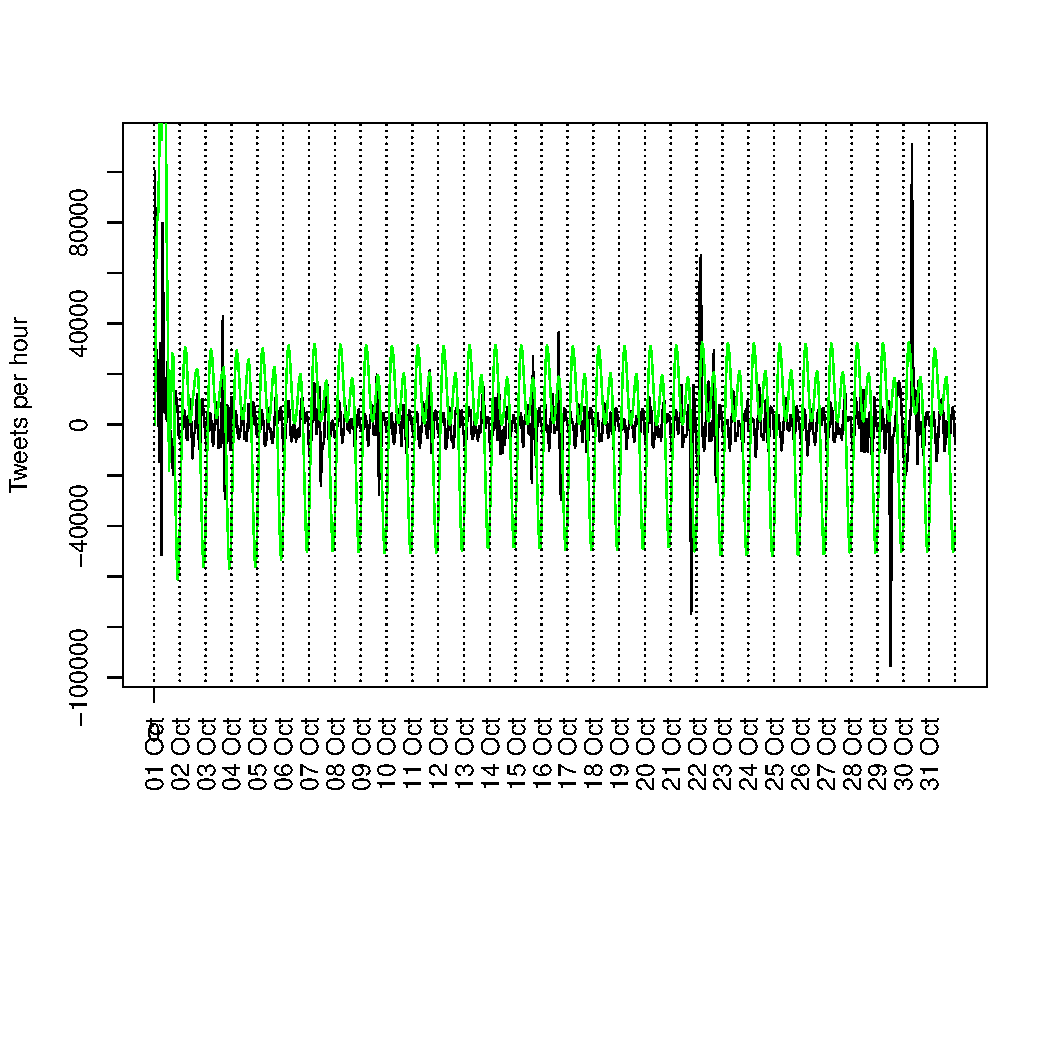
\includegraphics[clip=true,trim=0in 1.5in 0in 1in]
{data-plots_oct/random-walk+days_NUMTWEETS_irregular+repeating.pdf}
\caption{Seasonal and noise components of the volume velocity}
\label{fig:volvel1}
\end{figure}

\begin{figure}
\centering
\includegraphics%[clip=true,trim=0in 1.5in 0in 1in]
{data-plots_oct/random-walk+days_NUMTWEETS_level+sma.pdf}
\caption{Stochastic level of the volume velocity}
\label{fig:volvel2}
\end{figure}

\subsection{Dynamic Support Threshold}
%Nevertheless, it
It is necessary to 
%As mentioned earlier, a \emph{frequent itemset} is a set of items that occur together a number of
%times higher than a given threshold, called the \emph{support} threshold.
%We 
adapt the support threshold to the dynamicity of the volume velocity at
different times of the day.
If a ratio support threshold is used then this would not be needed,
however determining a support ratio is difficult 
and it is more desirable to be able to specify the threshold
as an absolute number. 
%To do this when the volume velocity is 
We therefore define the \emph{minimum support threshold} as the threshold at the hour
of the least volume velocity during the day.
The \emph{minimum support threshold} is supplied as an absolute number %, $a$, 
and then converted to a ratio, $\alpha$, % = \frac{a}{\textbf{avg}(\min_{day}{(vol.\, vel.)})}$.
by dividing it by the average of the number of tweets in the hour of minimum volume velocity in different days. 
The actual support threshold used for mining any given epoch, $E$, is thus
$\alpha$ multiplied by the number of tweets in the epoch: %'s volume velocity:
\begin{align}
dynamic\_support\_threshold &= \alpha \times |E|  \hspace*{1.2cm}  where\,\alpha: support\,ratio\\ %\frac{|E|}{E.span}
&= \frac{minimum\_support\_threshold}{\textbf{avg}(\min_{day}{(volume\, velocity)})} \times |E| %\frac{|E|}{E.span} 
\end{align}

Calculating the support threshold dynamically as such
makes it intuitive to select a minimum support threshold,
but it would lead to a high support threshold in epochs including a burst of tweets. % caused by any event.
%(peaks in the leve
%if a long epoch span is used the support might
%e support ratio is multiplied by the volume velocity of the epoch, 
The high support might lead to mining only itemsets
about the topic that is causing the burst.
 %,
%other topics will not be mined. 
%Stream processing methods %of computation
%can be used to alleviate this problem.
%To alleviate this problem
%mine epochs of 
%data
Mining a sliding window can alleviate this problem.



\subsection{Sliding Window Model}

One of the prominent stream processing models is the sliding window model,
where a window of  data  \emph{slides} forwards through the stream. 
The window keeps a fixed amount of history data (fixed in terms of age not size); 
data with a timestamp older that a certain time is removed from the window 
as new data is added. %just created 
The data in the window is processed every time the window slides.
Thus, the sliding window model sets a cut-off age after which
a datapoint has no effect at all on the results of the stream processing algorithm. % of the processing 
This is the simplest way to overcome the problem
that an anomaly in the date, 
such as a burst of tweets about a certain topic,
could affect the mining results more than recent data.
More elaborate methods include dynamically changing the 
sliding window size~\cite{bifet2007learning}, 
smoothing the data~\cite{gilbert2001surfing},
%storing approximate statistics (sketch)
and weighting data according to its age~\cite{giannella2003mining}.

We apply our algorithms to epochs of data, 
similar to the \emph{block evolution} stream mining approach~\cite{ganti2002mining,zhu2003efficient}.
However, our algorithms are not strictly stream processing algorithms.
Stream processing algorithms are supposed to process transactions one at a time
as they arrive, looking at each transaction only once
--~in other words, they should make one pass on the data then discard it.
This complicates the model of computation % a lot
and there is no justification to process social media data as a stream.
The stream processing model of computation is justified when
the data is not supposed to be stored (such as data from sensor networks),
or when the processing time has to be as short as possible 
such that looking at historic data is an overhead 
(such as in the case of processing stock ticker data, 
where making a decision a few milliseconds 
before/after competitors can translate into profits/losses).
%millions of dollars). 
In the case of social media text, 
the data has to be stored anyway 
and the perception of the human users
makes processing times in the order of seconds %or even minutes
acceptable for a \emph{real time} system.


%We can regard the way we process the social media stream as 
In essence, processing epochs of data is similar to %still 
mining a sliding window that is moved forward by time steps of short span.
The time step must be longer than the time needed to mine an epoch of data,
and the performance of our algorithms makes it possible to use a time step
as short as a few seconds for epochs up to a day long.
The window must be moved such that the combinations of
transactions not processed together in a batch is minimal.
This is achieved by using a time step as short as possible, 
within the limits of available resources
(such as storage space for mining results, if they are retained).
Moreover, the time step must be less than the epoch length
%cannot exceed half of the epoch length,
%if it does, 
to avoid missing mining results from a spike % of what?
happening at the boundary between two epochs.


Figure \ref{fig:runtimeEpochs} shows the runtime of LCM on epochs of
increasing length, and we will show in section \ref{sec:effic} that our
extensions do not degrade its performance.
The times reported in figure \ref{fig:runtimeEpochs} are averages across all
epochs of the specified length in the last 3 months of 2012, % October, November and December,
using a time step that is half the epoch length.
The variance is very low and the confidence bands are not shown because they
appear as dots.  % on top of the bars. 
The \emph{minimum support threshold} used throughout this thesis %, unless otherwise specified,
is 10 occurrences in the hour of day in which the volume velocity is the minimum. % $\alpha=0.0002$.
Figure \ref{fig:avgSupp} shows the averages of the actual support threshold to which this minimum support
threshold translates at different epoch spans.

\begin{figure}
\centering
\scalebox{0.4}{
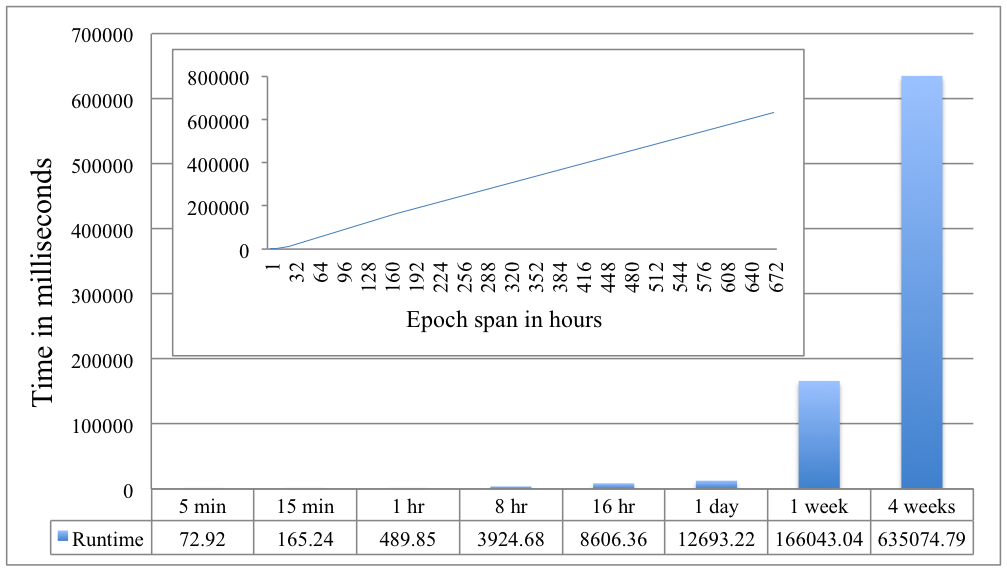
\includegraphics{runtim_epoch-spans_line-over-bars.png}
}
\caption{Mean runtime of LCM at different epoch spans}
\label{fig:runtimeEpochs}
\end{figure}


\begin{figure}
\centering
\scalebox{0.9}{
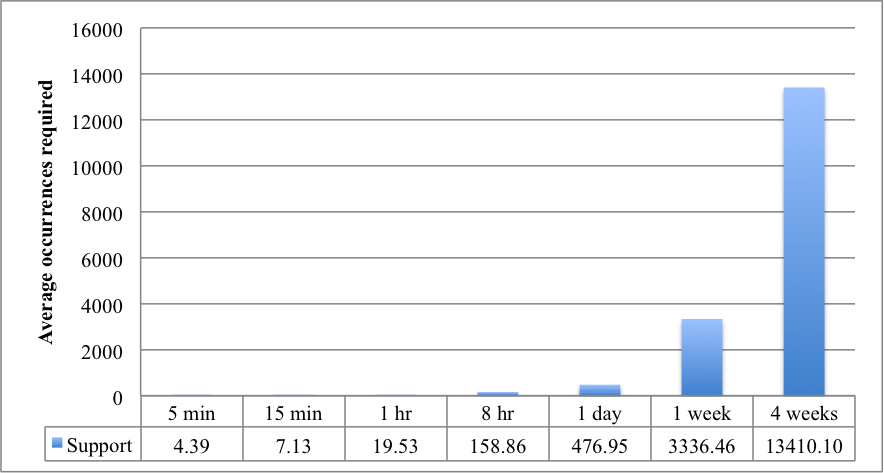
\includegraphics{epochlen_support.png}
}
\caption{Mean support corresponding to minimum support 10, at different epoch spans}
\label{fig:avgSupp}
\end{figure}

%TODONOT elaborate on that.. show figures.
\newpage
In the rest of this paper we mine epochs of 1 hour span.
The reason behind this choice is an observation that the number of closed
itemsets mined from epochs of span 1 hour or more,
at the same minimum support threshold, 
remains the same.
This indicates that itemsets mined from shorter epochs % of social media text
are not included in the results of mining longer epochs. 
Therefore, the epoch span should be minimized.
However, when the epoch span is shorter than an hour the frequency required
to surpass the support threshold becomes very low,
and the number of mined itemsets increases, 
with many noise itemsets appearing in the results.
%Figure \ref{fig:epochLenNumItemsets} shows the number of 
%closed itemsets at different epoch lengthes.. maximal ones too.. but using N-Gram 5.
%For example, the number of itemsets is doubled
%when the epoch length is reduced to 15 minutes instead of an hour.
For example, the number of itemsets mined from a 15 minutes epoch
is double that mined from an hour long epoch.

Regardless of the length of the epoch,
many mined itemsets are combinations of function words.
In the next section, we outline how we reduce the number of itemsets and
eliminate the effect of function words by N-gram filtering.

\section{Filtering Language Constructs}
%\subsection{Tokenizing into Variable Length N-grams}
\label{sec:ngrams}

A large number of itemsets are language constructs that bear no information,
such as ``such as''. 
By treating sequential language constructs, and any other multiword expression,
as one item we eliminate a large number of such itemsets.
We can also eliminate itemsets that are made up of all the different fragments
of the language construct along with other items;
for example, the itemset \{we, did, it, \#teamobama\} can produce 10 other combinations of
length 2 or more.
There are many measures of association that can be used to detect multiword
expressions, but each measure is good only under certain conditions~\cite{ramisch2012broad}.
After preliminary experiments with various measures, we determined that
the best performance
could be obtained by tokenizing the documents into term N-grams 
of varying length.
%with varying N. 


We use term N-gram tokens such that N-grams of high probability are replaced by
(N+1)-grams, resulting in a distribution with no high peaks.  
An N-gram is considered to % of length N
have a high probability if its maximum likelihood estimate, 
from a background model,
is higher than a threshold $\eta_N$. 
A background language model built from a long epoch of data 
from the same stream is used for probability estimation.
The language model is simply a hash map of the counts of 
N-grams that appeared within the last month, for N up to 7.
% In reality the N-grams probabilities come from the same 
% epoch, but this is probably a mistake on my side.. 
% or maybe it was one thing done right by mistake..
% or maybe I tried having a background model and found it
% not satisfactory (no i didn't).

\newpage
The tokenization of a tweet starts by tokenizing it into unigrams, 
as described in appendinx \ref{AppendixA}. % the next section. % \ref{sec:tokenization}.
Then, each
unigram of high probability is replaced by two term bigrams, by
attaching to it the unigrams before and after it.
We keep replacing N-grams of high probability by two (N+1)-grams 
%repeat this for each N $\ge$ 1,for all N-grams
%with probabilities above the threshold 
until there are no more such N-grams. %; thus, the distribution is relatively flat.

The threshold of high probability is different for each value of N. 
The threshold for unigrams is determined as follows: 
We pick a topical term that is known to  steadily  appear with a rather high frequency, 
and is talked about in all languages; for example, `obama'. 
The maximum likelihood estimate of the probability of the term `obama' within the whole collection of tweets is 0.0001. 
%in a similar fashion to how we determined the support threshold. 
We use $\eta_1 = P(``obama") = 0.0001$.
At each N, the probability threshold is adjusted to account for the increase
in the number of tokens and the overall increase in the grand sum of counts (caused by overlap).
The adjusted $\eta_N$ is:
\begin{equation}\eta_N = \eta_1 \times \frac{\sum_{\{w:\, w \,\in\, W\, and\, w.length \,\le\, N\}}{freq(w)}}{\sum_{\{v:\, v\, \in\, W \,and \,v.length\,=\,1\}}{freq(v)}}\end{equation}

The effect of increasing the maximum length of N-grams %from 1 to 5 
is shown in figures \ref{fig:ngramsDist} and  \ref{fig:ngramsLen}.
Figure \ref{fig:ngramsDist} shows the flattening of the distribution
by plotting the average decile values at three different times of day. 
N-grams appearing less than 10 times in an hour
(the minimum support threshold we use) are excluded,
because they do not contribute to the distribution of items
that the algorithm has to mine.
The peakedness of the head of the Zipfean distribution 
is reflected in the peakedness of the $100^{th}$ percentile.
%As the maximum N increases
Increasing the maximum N-gram length 
reduces the peakedness  as well as 
the variance in the peakedness between different
hours of day.
%~--~ the difference between the maximum 1-gram frequencies 
%at different hours of day is in the order of thousands.
Figure \ref{fig:ngramsLen} shows how the maximum N-gram length
affects the mining algorithm; it shows
the number of tokens in the input, the number of closed itemsets,
%of length more than 1, 
and the runtime of mining one hour of data.
The values shown are averages across all one-hour epochs in the month of
November 2012.
The value of $\eta_1$ used is 0.0001.
Figure \ref{fig:ngramsLen}(a) shows that the number of distinct items
increases substantially as the maximum N-gram length
increases from 1 to 2, then continues increasing
slightly until it starts decreasing at $N \le 5$.
The decrease happens because all 4-grams with probability above the threshold
are parts of tweets from services that use the same text and append a URL,
such as tweets reporting scores from
Game Insight\footnote{\url{http://www.game-insight.com/}}.
Such tweets are tokenized into more 4-grams than 5-grams, and the 4-grams
appearing in them do not appear elsewhere.
%Thus, each three adjacent 4-grams are replaced by two 5-grams.
Thus, some adjacent 4-grams are replaced by fewer 5-grams.
Figure \ref{fig:ngramsLen}(b) shows that the number of itemsets continues to
decrease as expected, with the biggest reduction when the maximum N-gram length
increases from 1 to 2.
Figure \ref{fig:ngramsLen}(c) shows that runtime also decreases as
the maximum N-gram length increases
from 1 to 5, since LCM's runtime is proportional to the number of closed
itemsets, and it %is not affected by the sparsity of data.
can take advantage of the sparsity of data.
The runtimes in this figure are slightly less than those in
figure \ref{fig:runtimeEpochs} because they do not include the time taken for
writing the posting list of each itemset.

The numbers of itemsets reported in the plots 
are counts of distinct unigram sets.
After mining itemsets of term N-grams we flatten the itemsets to sets of unigrams again.
This is necessary since an itemset will have different N-gram set representations,
and its postings list is the union of those of the different representations.
%Flattening N-gram itemsets into unigram itemsets
This
also removes overlap between N-grams of the same itemset,
making it easier to reason about how itemsets relate to each other.
We will use the relation between an itemset and its subsets to
select interesting itemsets in the next chapter.

%The counts include itemsets of length 1 (frequent unigrams).
The condition for selecting itemsets that we propose in the next chapter
cannot select itemsets of length 1 (frequent unigrams).
Thus, to assess its filtering characteristics we have to 
compare the number of itemsets it selects to 
the number of itemsets of length 2 or more before its application.
At $N \le 5$, the number of \emph{closed itemsets} of length 2 or more
that are mined from an hour long epoch averages at 2,439.17.
We also note that the number of \emph{maximal itemsets} of length 2 or more
averages at 1,831.92.
This high number of \emph{maximal itemsets} 
show that they cannot substitute
the \emph{strongly closed itemsets},
%even though
which we propose in the next chapter.
%which shows that there aren't many internal nodes
%in the itemset prefix tree 
%%when items are ($N \le 5$)-grams
%(recall that closed itemsets include maximal itemsets).


%filter out uninformative itemset 


%Notice that the (N+1)-grams replacing an N-gram overlap with each other, with the unigrams that got 
%attached to the N-gram and possibly with other N-grams. 
%However, the  
%We do not prevent overlap, because there is no guarantee that the N-Gram
%created makes any sense.After mining term N-grams we flatten the itemsets to sets of unigrams again.
%This removes overlap between parts of itemsets making it easier to reason
%about how they relate to each other. 
%This is also necessary since an itemset will have different N-gram set
%representations,
%and its postings list is the union of those of the different representations.


\begin{figure}
\centering
\scalebox{0.6}{
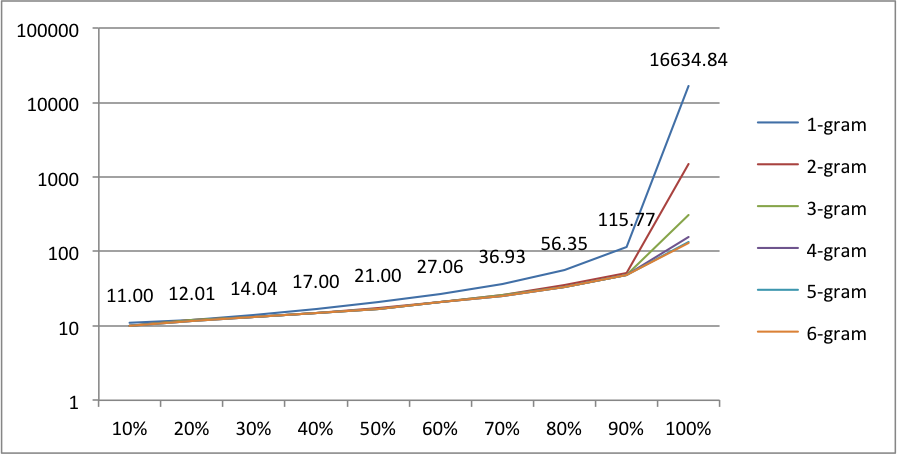
\includegraphics{examples/deciles_ngrams1-6_3hod-max_00-01_wvalues.png}
}
\\
\begin{tabular}{c}
\\(a) Hour of Day: 00-01 HST (5-6 AM EST) \\ \\
\end{tabular}
\\
%\caption{Mean number of distinct items}
%\label{fig:ngramsLenA}
%\end{figure}
%\begin{figure}
%\centering
\scalebox{0.6}{
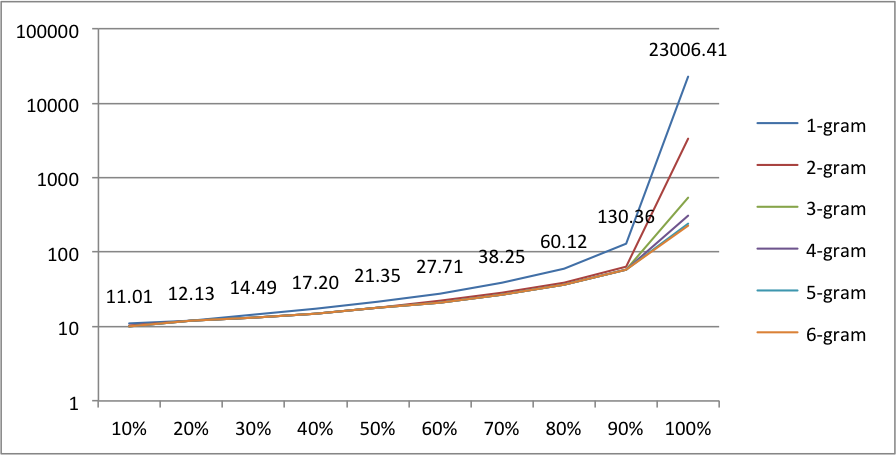
\includegraphics{examples/deciles_ngrams1-6_3hod-max_08-09_wvalues.png}
}
\\
\begin{tabular}{c}
\\(b) Hour of Day: 08-09 HST (1-2 PM EST) \\ \\
\end{tabular}
\\
%\caption{Mean number of itemsets}
%\label{fig:ngramsLenB}
%\end{figure}
%\begin{figure}
%\centering
\scalebox{0.6}{
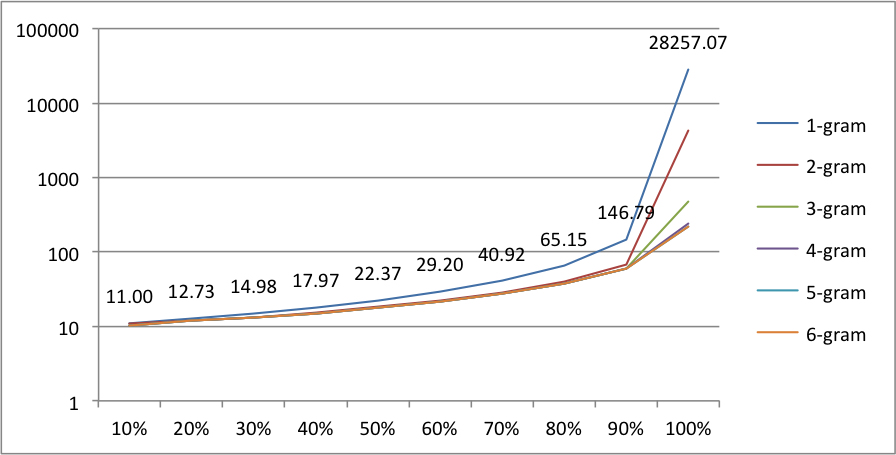
\includegraphics{examples/deciles_ngrams1-6_3hod-max_16-17_wvalues.png}
}
\\
\begin{tabular}{c}
\\(c) Hour of Day: 16-17 HST (9-10 PM EST)
\end{tabular}
%\caption{Mean runtime in milliseconds}
%\label{fig:ngramsLenC}
\caption{Average of token frequency percentiles at different times of day and maximum N-gram length}
\label{fig:ngramsDist}
\end{figure} 



\begin{figure}
\centering
\scalebox{0.78}{
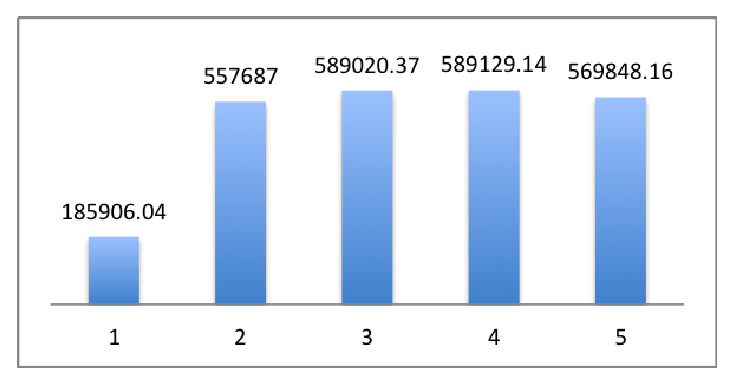
\includegraphics{perf_ngramlen1-5_distinct-items_supp10+_1hr.eps}
}
\\
\begin{tabular}{c}
\\(a) Mean number of distinct items at different values of maximum N \\ \\
\end{tabular}
\\
%\caption{Mean number of distinct items}
%\label{fig:ngramsLenA}
%\end{figure}
%\begin{figure}
%\centering
\scalebox{0.78}{
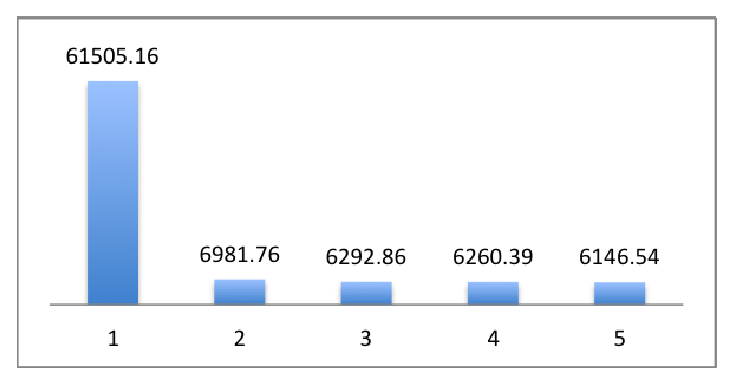
\includegraphics{perf_ngramlen1-5_itemsets_supp10+_1hr.eps}
}
\\
\begin{tabular}{c}
\\(b) Mean number of itemsets at different values of maximum N \\ \\
\end{tabular}
\\
%\caption{Mean number of itemsets}
%\label{fig:ngramsLenB}
%\end{figure}
%\begin{figure}
%\centering
\scalebox{0.78}{
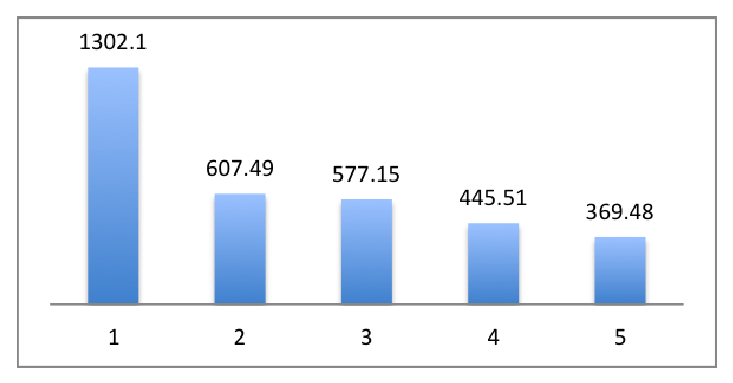
\includegraphics{perf_ngramlen1-5_runtime-millis_supp10+_1hr.eps}
}
\\
\begin{tabular}{c}
\\(c) Mean runtime in milliseconds at different values of maximum N
\end{tabular}
%\caption{Mean runtime in milliseconds}
%\label{fig:ngramsLenC}
\caption{Effect of changing the maximum N-gram length on mining hour long epoches}
\label{fig:ngramsLen}
\end{figure} 





% =========================================
% C H A P T E R     4
% =========================================

\chapter{Selecting and Ranking Itemsets} %Selecting Interesting
\label{sec:strong}

In section~\ref{sec:ngrams}, we discussed our handling of function words,
using a technique that exploits LCM's tolerance to sparsity.
After applying this technique, the average number of closed itemsets 
mined from an
hour of Twitter data drops from 61,505 to 6,146.
In this chapter we propose two methods
for reducing the number of itemsets even further.
The first is a condition for selecting itemsets,
% that filters out some itemsets,
and the second is a clustering scheme that merges together
similar itemsets to reduce redundancy.
We also propose a ranking function that
scores itemsets according to their temporal novelty.
The two methods and the ranking function all
exploit the dynamics of social media,
therefore we start by discussing it.
%and specifically how people use retweeting
%to surface important 
%that do not carry 
%more itemsets
%that are 
%However, many  frequent N-grams are flatte
%there is still redundancy in the itemsets.

\section{Social Media Dynamics}

As discussed earlier, one use case of social media %users 
is to
share content that a user finds important with her network.
%surface important content through sharing it.
The user may share an original status message about the 
topic of interest, or \emph{re-share} content posted by other users.
In twitter, re-sharing is done by retweeting,
which can be done in several ways.
One way is by using the ``retweet'' feature of the Twitter client,
which simply forwards the tweet to the user's network.
The ``retweet'' feature keeps a reference to the original tweet
in the forwarded tweet, but it does not allow editing it
--~it automatically prepends ``RT: @\emph{orignal\_poster\_username}''.
%The retweet feature was introduced
%Only a small fraction of retweets are forwarded using the 
%``retweet feature
Since editing is not supported by the ``retweet'' feature, 
many users chose to retweet manually 
to be able to add their own thoughts.
Recently this can be done using the ``reply'' feature,
which allows a user to write a tweet 
that references the original tweet
thus
maintaining the hierarchy of the conversation.
However, manually retweeting is still a prevalent
way to re-share a tweet along with the user's comment.

%originally there was no way to link a certain tweet to another,
%thus a tweet that sparked a conversation on Twitter 
There are several conventions for manual retweeting~\cite{boyd2010tweet}. %\emph{styles} 
%They are all basically to
All the conventions basically
quote the original tweet along 
with its poster's username and a retweet indicator,
%and prepend the user's comment.
%had to be quoted in a retweet
%along with the retweeter's comment.
with the retweeter's comment prepended.
Due to the 140 characters limit set on the length of tweets 
the quotation is usually 
edited to be as short as possible 
by selecting only the most discriminative words. 
This selection is an act of collaborative filtering,
but it results in many trivially different subsets from the original tweet,
and all subsets with enough support will be mined as itemsets.
The additions of retweeters also form many different supersets of the of the
original tweet, and some additions may represent opinions that are supported
enough to be mined as itemsets. 


\begin{figure}
\centering
\scalebox{0.5}{
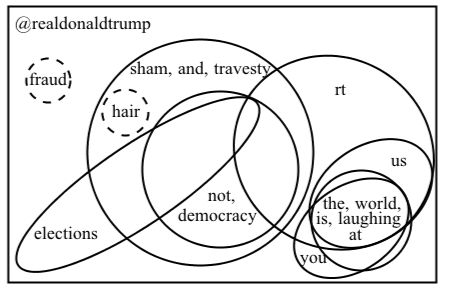
\includegraphics{sham.png}
}
\caption{Venn diagram of transactions containing items from highly retweeted tweets} % closed itemsets
\label{fig:sham}
\end{figure}

Figure \ref{fig:sham} illustrates closed itemsets related to two of
Donald Trump's famous tweets in reaction to Obama's victory in the
2012 US elections\footnote{\url{http://www.huffingtonpost.com/2012/11/07/donald-trump-election-revolution_n_2085864.html}}.  
Each area in the figure represents the transactions containing the itemset
formed by concatenating the items in all intersecting ellipses.  
%In the figure, the most discriminative words are ``sham, and, travesty''
The figure shows that one of the tweets was most distinguishable by the words ``sham, and, travesty'',
which are quoted along with Donald Trump's user name in most of the retweets.
Other people also chose to include ``not, democracy'' and/or ``elections'' in their retweets,
and in most of the cases the retweet indicator ``rt'' was added to the retweet. 
A few people also added something about Donald Trump's ``hair'' 
while retweeting.
The second tweet's most discriminative words are ``the, world, is, laughing, at''.
Some people completed this by the original tweet's ``us'',
and others replaced it by ``you''.
At the same time interval, some people tweeted about ``fraud'' 
mentioning Donald Trump in their tweets
but without any quotation from his tweets. 

The figure illustrates how
the closed property of an itemset is easily satisfied by an itemset
created through the modification of 
transactions that contain another closed itemset.
For example, if a transaction containing a closed itemset
is modified by removing one of its items,
another closed itemset with enough support is immediately formed
resulting in a two closed itemsets instead of one.
While an update operation is not supported in the model of frequent itemset mining, 
a similar effect happens when people retweet, 
or even when they are writing original posts about 
a certain fine grained topic.
In case of retweeting, people actually start from the original tweet and 
then remove parts of it to make space for their content. 
We can imagine that for each fine grained topic there is also a base post
that represent the information or ideas within the topic. 
People make posts about the fine grained topic 
by selecting parts of the base post
and adding their own thoughts.
This results in many closed itemsets 
about the topic that
are trivially different from each other.
%We now propose a condition that exploits this 

The fact that any \emph{maximal} itemset is a closed itemset
is another \emph{weakness} of the closed condition
when used for mining social media text.
%If an item is added to a number of retweets higher than the support threshold
%it results in a \emph{maximal} itemset.
%The itemset will be closed by definition even if the support threshold
%is much lower than the total number of retweets
If a closed itemset is expanded by a certain item a number of times
over the support threshold, this results in a maximal itemset
which is closed by definition.
%If the support of the original itemset is much higher than the support threshold,
%the newly created itemset might not 
%but might not be carrying 
%if the support 
%threshold is much lower than the 
%Now consider that in social media a low support threshold has to be used.
Now consider that a tweet is retweeted hundreds of times 
%resulting in some closed itemsets,
and different groups of people append the same words to it,
but no group is considerably large relative to the number of retweets.
Since  a low support threshold has to be used when mining text,
this will result in many maximal itemsets that 
might not be adding any information to the closed itemset.
%If the support threshold is around 10, 
%would a maximal itemset certain comment added by 10 people be worth 

%enough tweets add the same  similar effect happens

\section{Distinct Itemsets}

We have seen that the dynamics of posting on social media result in redundant closed itemsets.
To reduce redundancy, we propose the \emph{distinct} condition,
which is not as easily satisified %violated  
as the closed condition, and use it for selecting itemsets.
The \emph{distinct} condition builds on the concept of \emph{association rule confidence}.
Confidence is the basic property used for association rules mining,
and it is used in the definition of $\delta$-free sets~\cite{boulicaut2003free}.
Mining itemsets based on the confidence of rules they induce has long been
recognized as a method for finding
``interesting patterns''~\cite{cohen2001finding},
but since this property is not anti-monotone it cannot be directly used
to mine itemsets. It has to be used in a post-processing phase.
%a variation has to be used
%(for example, \emph{all confidence}). % \cite{kim2004ccmine}
The confidence of an assocation rule that the presence of an itemset,
$s_{antecedent}$, implies the presence of another itemset, $s_{consequent}$, is  defined as:
\begin{equation}\label{eq:conf}conf(s_{antecedent} \rightarrow s_{consequent}) = \frac{|T_{s_{antecedent}} \cap T_{s_{consequent}}|}{|T_{s_{antecedent}}|}\end{equation}


The \emph{distinct} condition is a novel strengthening of the closed condition
so that it is not easily satisfied by any modification of a closed itemset. %modification??
%violated by trivial differences.
%A closed itemset of length $k$, call it $s_p$, % with high support %(say 100 occurrences in an hour)
%can have as many frequent supersets of length $k+1$ as its support, %divided by the support threshold,
%where $s_p$ will be the intersection of the supersets.
%From the properties of closed itemsets, 
%each superset that has enough support
%will result in one or more closed itemsets;
%if a superset is a maximal itemset then 
%it will result in only one closed itemset,
%and if it can be extended further it will 
%result in more closed itemsets.
%Now consider that $s_p$ has a particularly high support,
Consider a closed itemset $s_{antecedent}$ that has a particularly high support,
as is the case for itemsets made up of the 
most discriminative words of a certain topic,
or a language construct used in different topics.
In this case, we can filter out
closed supersets of $s_{antecedent}$ that have
support high enough to satisfy the support threshold
but much lower than $s_{antecedent}$'s support.
These itemsets have enough support to be mined as frequent itemsets, 
%and they are closed because they have a closed subset, 
but they do not represent 
a \emph{distinctive} piece of information or opinion 
within the topic that $s_{antecedent}$ represents.
%The same reasoning can be applied to 
%an itemset that is created by removing 
%Note that this reasoning applies

The \emph{distinct} condition is similar in essence to mining itemsets
at multiple minimum supports~\cite{liu1999mining,seno2005finding,wang2000mining,xiong2003mining}, 
where a different support threshold is used for 
%different categories of items according to their relative frequency.
each itemset according to the frequency of its components, or its length, 
or some other function that calculates the \emph{suitable} support threshold.
However, \emph{distinct} itemsets are based on a very simple condition
that is easy to implement efficiently and intuitive to reason about.


We define a \emph{distinct} itemset as a closed itemset whose frequency
comprises more than a certain proportion of the frequency of its least
frequent subset~--~we call this its \emph{parent} itemset. 
%This condition chooses closed itemsets which substantially violate the closed
%condition of their subsets.
The proportion is a parameter, $\kappa$, that controls the selectivity 
of the condition,
or the \emph{distinctiveness} of itemsets selected by the condition.
This can be interpreted as selecting itemsets which are implied by a subset
with confidence greater than $\kappa$.
Formally, the set of \emph{distinct} itemsets, $\mathcal{D}$,
is defined as follows:
\begin{equation}\mathcal{D} = \{s: s \in \mathcal{C} \, and \, \exists \; s_{parent} \subset s \; where \; \frac{|T_{s}|}{|T_{s_{parent}}|} \ge \kappa 
\}
\end{equation}


%To assess the filtering power of the \emph{distinct} condition
%and make sure that no important information is filtered out, 
%we calculate the difference between 
%we compare the sizes of 
%the set \emph{distinct} itemsets ($\kappa = 0.25$)
%with
%the set of closed itemsets of length 2 or more. 
In the mining results of hour long epochs from the 
%first two weeks of November 2012, 
Twitter data,
the number of \emph{distinct} itemsets, at $\kappa = 0.25$,
%averages at 911.71 itemsets without setting a limit on the number of itemsets to keep
averages at 347.01 itemsets
%as compared to 2,428.3 closed itemsets.
%(37.55\%). 
as compared to 2,439.17 closed itemsets of length 2 or more.
To make sure that no important information is filtered out
we look at itemsets that are filtered out,
and
to facilitate the investigation we restrict it to %look at
itemsets containing one of the topical terms `obama' or `romney'
in the first two weeks of November 2012.
%In the mining results of hour long epochs from the 
%first two weeks of November 2012, 
%The number of closed itemsets
%containing 
%a topical term
%at least one of the unigrams 
%`obama' or `romney' 
%but are not \emph{distinct} 
%averages at 7.2 itemsets
%--~an epoch is included in the average only if a keyword occur in it.
%These are mainly 2-itemsets.
Excluding epochs in which the terms do not occur at all,
the average number of filtered out %(closed but not \emph{distinct})
itemsets that contain a topical term 
%by are not 
%that are not distinct 
is 7.2 itemsets per epoch.
The hour when 
the US presidential elections result became clear
%of the 2012 US presidential elections victory announcement
(10 PM EST on 6 November, 2012)
happens to be the hour with the most number of such itemsets, 
because of the large number of posts about `obama' and `romney'.
Figure \ref{fig:closedNDistinct} shows
the filtered itemsets from this hour.
%between closed and and 
Most of the itemsets in the figure are not interesting.
Furthermore, interesting ones have surrogates
in the set of \emph{distinct} itemsets:
%either 
a subset or a superset or an alternative 
with similar (sometimes more accurate) information.
In the figure, 
%the \emph{distinct} surrogate for each filtered itemset 
%that we find interesting is shown below it.
we include below each filtered itemset that we find interesting 
the \emph{distinct} itemset that we consider its surrogate.

%To generate the diff:
%java -cp target/diff_itemset-collections-0.0.1-SNAPSHOT.jar yaboulna.fpm.Diff /home/yaboulna/fim_out/lcm_closed_thesis/1hr+30min_ngram5-relpp10_oct-nov-dec highConf_June16Defaults_NoLonely_conf0.25_Buff1000_ novel_June16Defaults_NoLonely_conf0.25_Buff1000_
%To find the surrogates:
%

%(below it with an arrow).
\begin{figure} %[h]
\centering
\footnotesize
\begin{minipage}[t]{0.33\textwidth}
1 [romney, that] \\
      2 [still, obama, is] \\
      $\hookrightarrow$  [still, obama] \\
      3 [romney, what] \\
      4 [romney, with] \\
      5 [will, romney] \\
      6 [romney, if, wins] \\
      7 [romney, for, mitt] \\
      8 [romney, lost] \\
     9 [romney, like] \\
     10 [romney, campaign] \\
     11 [romney, is, mitt] \\
     12 [romney, still] \\
     13 [romney, supporters] \\
     14 [romney, a] \\
     15 [romney, i] \\
     16 [s, romney] \\
     17 [romney, of] \\
     18 [romney, on] \\
19 [romney, or]

     20 [romney, in] \\
     21 [romney, is] \\
    22 [romney, had] \\    
     23 [romney, at] 

        \end{minipage}
\begin{minipage}[t]{0.33\textwidth}

     
     24 [romney, 244] \\
       $\hookrightarrow$  [obama, 244] \\
     25 [romney, has] \\
     26 [romney, got] \\
     27 [romney, can] \\
     28 [romney, but] \\
     29 [romney, was] \\
     30 [romney, the] \\
     31 [voted, for, obama, who] \\
     32 [2012, obama] \\
     33 [romney, aint] \\
     34 [obama, is, barack] \\
     35 [gana, obama] \\
     36 [obama, gano] \\
   37  [michelle, obama] \\
  39 [years, more, obama, 4] \\
   $\hookrightarrow$  [\#4moreyears, obama] \\
     40 [romney, for, vote] \\ 
     41 [de, obama] \\
     42 [obama, an] \\
     43 [on, obama] \\
     44 [obama, it] \\
     45 [so, obama] \\
     46 [obama, d] 
         
\end{minipage}
\begin{minipage}[t]{0.3\textwidth}

     
     47 [did, obama, it] \\
     48 [for, obama, it] \\ 
     49 [que, obama] \\
     50 [URL, obama] \\
     51 [can, obama] \\
     52 [obama, all] \\
     53 [so, obama, won] \\
     $\hookrightarrow$ [wonnn, obama] \\
     54 [yes, obama] \\
     55 [obama, is, the] \\
     56 [supporters, obama] \\
     57 [obama, when] \\
     58 [with, obama] \\
     59 [obama, team] \\
     60 [obama, has, won] \\
     $\hookrightarrow$ [obama, we, won]\\
     61 [this, got, obama] \\
     62 [yeah, obama] \\
     63 [romney, about] \\
     64 [obama, happy, won] \\
    $\hookrightarrow$ [glad, obama, won] \\
     65 [yesss, obama] \\
     66 [president, obama, barack] 
\end{minipage}
\caption{Itemsets  from the hour starting at 10 PM EST on 6 Nov. 2012,
which contain `barack' or `romeny' and are closed but not \emph{distinct}}
\label{fig:closedNDistinct}
\end{figure}

In figure \ref{fig:sham}, \emph{distinct} itemsets are illustrated in solid lines, 
and closed itemsets that do not satisfy the distinctiveness condition are illustrated in dashed lines.
This is not an accurate illustration and it is only meant 
to give an intuition of how \emph{distinct} itemset are different from closed itemsets which are not \emph{distinct}.
%Figures \ref{fig:winningHr} and \ref{fig:closedNDistinct} 
%are realistic examples of itemsets that are selected or 
%rejected by the \emph{distinct} condition.
%Both figures show itemsets from the hour .
%The \emph{distinct} condition was applied at $\kappa = 0.25$.
We have seen in figure~\ref{fig:closedNDistinct} some realistic
examples of itemsets that are rejected by the \emph{distinct} condition.
Figure~\ref{fig:winningHr} shows the \emph{distinct} itemsets % it selects
from the same hour at the same $\kappa$.
%The itemsets shown are \emph{distinct} at $\kappa = 0.25$.
%Each itemset has its support next to it, 
%The figure is produced by the graph drawing algorithm proposed by Yifan Hu~\cite{hu2005efficient},
%using the implementation provided 
%in the graph visualization platform Gephi\footnote{\url{https://gephi.org/}}.
%We run the algorithm on a graph with a node for each itemset and 
%an edge between similar itemsets.
%Similarity between itemsets
%is determined based on 
%association rule confidence,
%The using the formula introduced in the next section. % of the rule that the smaller set 
%as explained in the next section.
%The similarity is used as the edge weight,
%thus it determines the distance between itemsets.
%Even though the support threshold There are
%The figure shows a lot of interesting itemsets.
%Figures \ref{fig:winningHr} shows the \emph{distinct} itemsets from that hour.
%Itemsets pertaining to Donald Trump's tweets appear on the right side of the page,
%where the itemsets from the ``sham and travesty'' tweet are in the middle.
%Barack Obama (BO) also made an 
%Other clusters of itemsets are easy to guess what they are about.
Itemsets pertaining to
Donald Trump's ``sham and travesty'' tweet appear on the right side of the figure.
Close to the bottom left of the figure there are itemsets showing the number
of electoral votes each candidate got at different points of time (\{191, 238\} and \{191, 249\}). 
%\footnote{https://plus.google.com/+NBCNews/posts/gNw1sYLWtE8}
It is clear from the figure that considerable redundancy remains in
\emph{distinct} itemsets. 
%However, most interesting itemsets
In the next section we propose overcoming this redundancy 
by clustering similar itemsets together.


\begin{landscape}
\begin{figure}
\centering
\scalebox{0.75}{
\frame{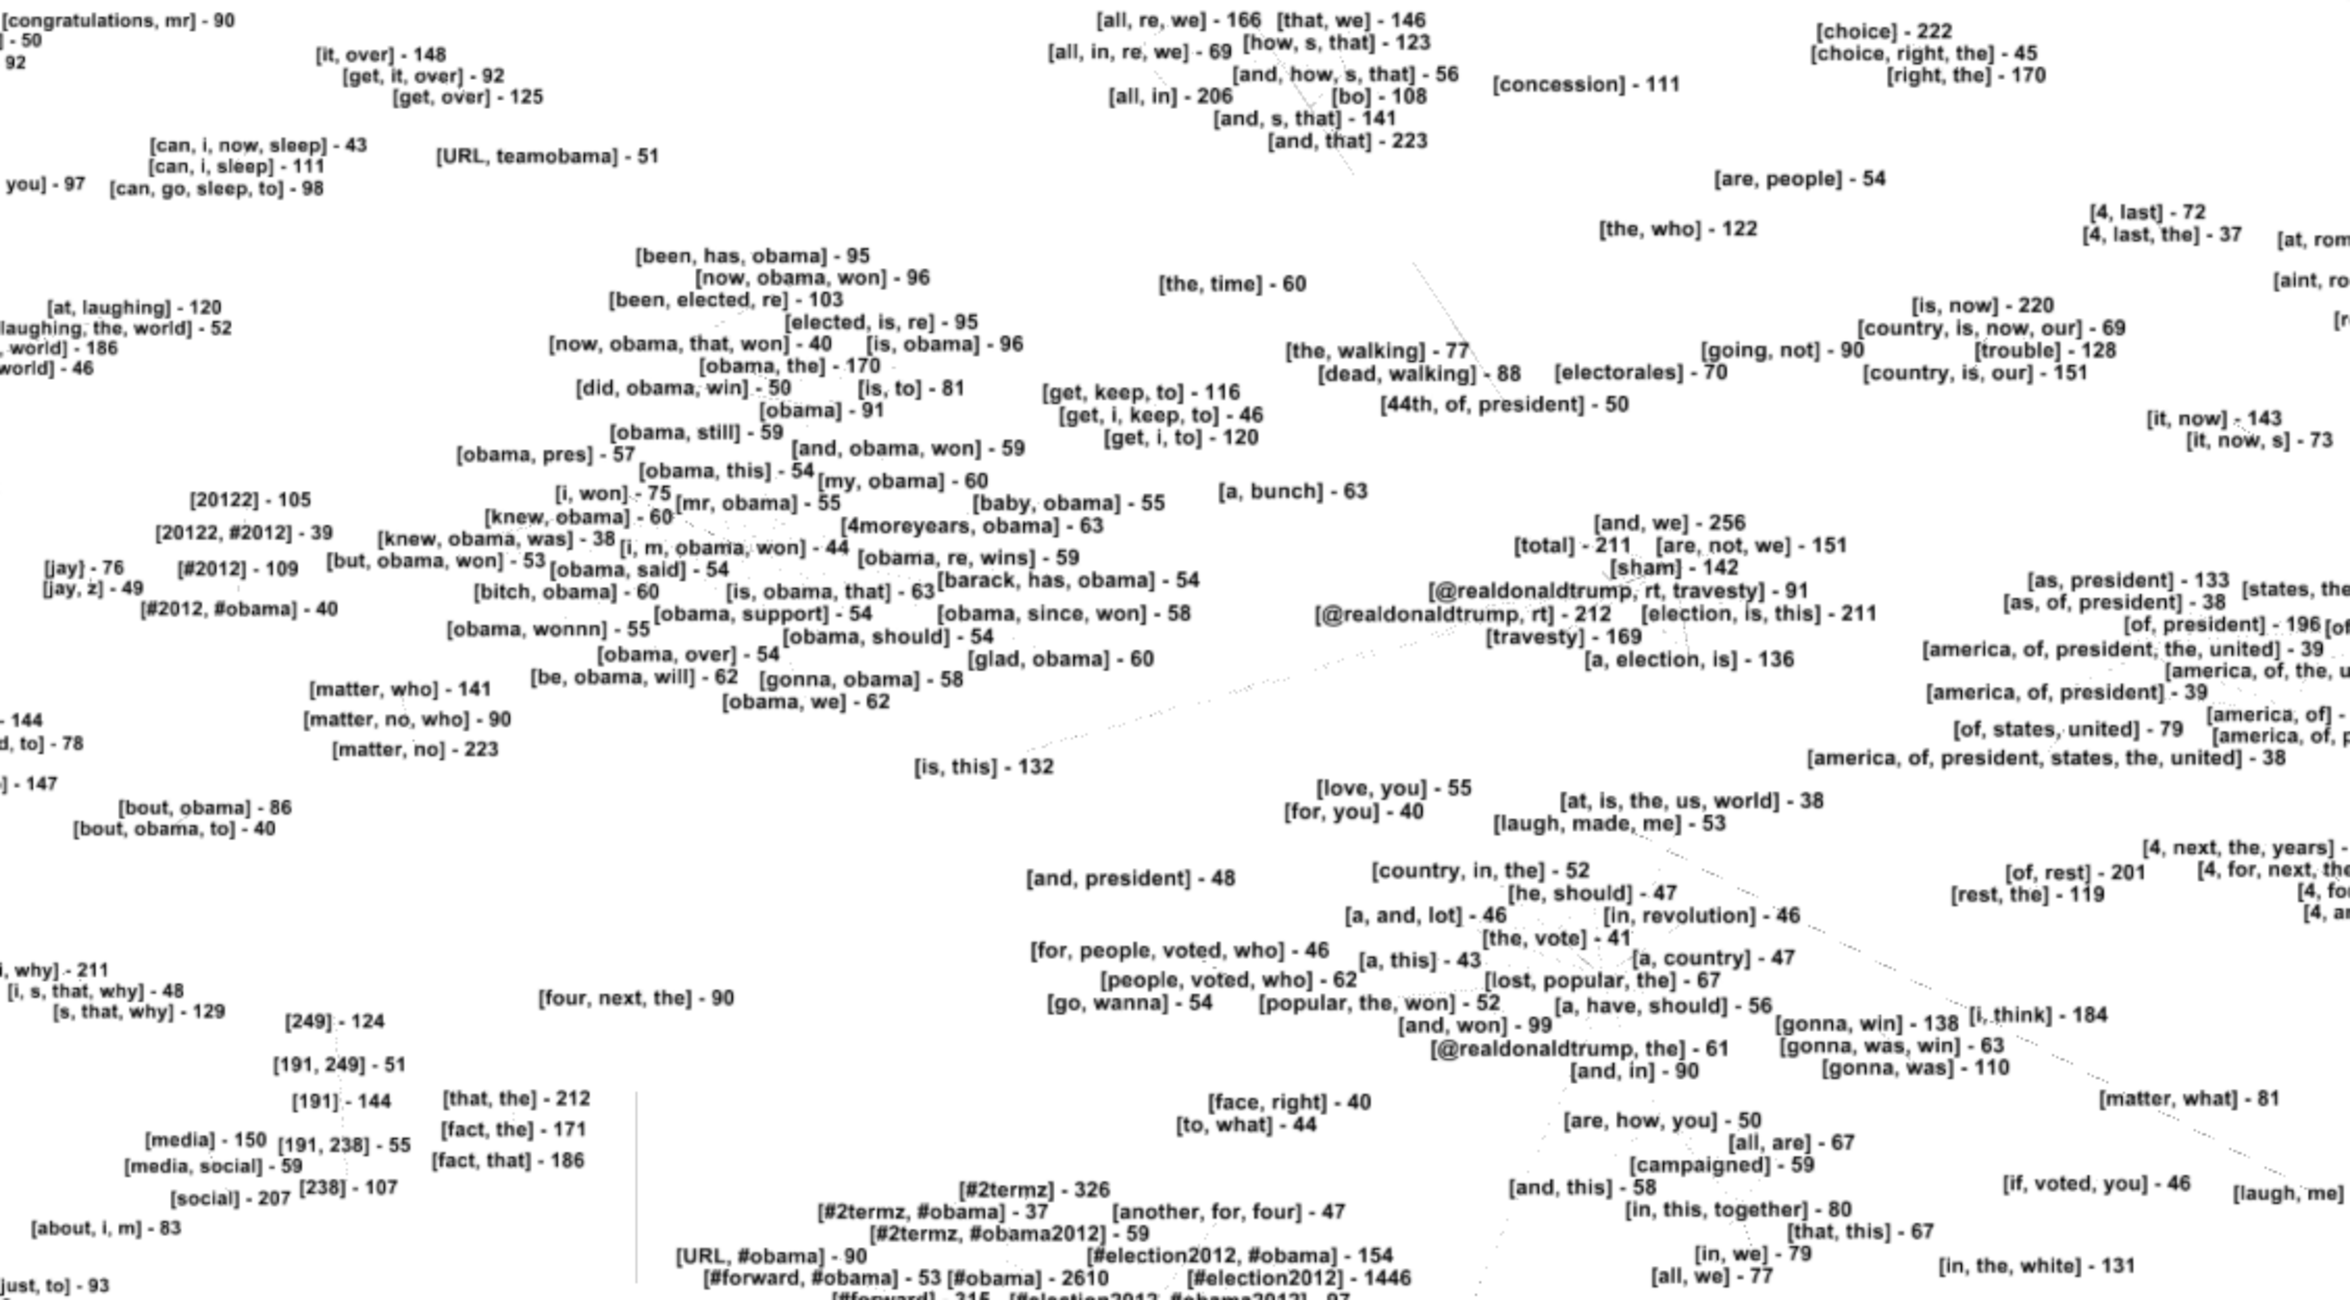
\includegraphics[trim=1in 0 3in 0, clip=true]{clustering/elections-day_10pm-est_2.pdf}}
}
\caption{Scatter plot of \emph{distinct} itemsets from the hour starting at 10 PM EST on 6 Nov. 2012 }
%(US Presidential Elections day)
\label{fig:winningHr}
\end{figure}
\end{landscape}




%wc -l diff_bieber-fox-romney-israel-hamas-syria-cnn-gomez-obama-trump_novel_ULBuff_Canddist_conf0.25_-sel_ULBuff_Canddist_conf0.25_3600_1352* | less -NS
%556  1811 total

%wc -l diff_NO-KEYWORDS_novel_ULBuff_Canddist_conf0.25_-sel_ULBuff_Canddist_conf0.25_3600_1352* | less -NS
%556  843224 total

%wc -l diff_romney-obama_novel_ULBuff_Canddist_conf0.25_-sel_ULBuff_Canddist_conf0.25_3600_1352* | less -NS
% 556  1728 total
%157  1720 total after removing files of size 0

%wc -l sel_ULBuff_Canddist_conf0.25_3600_1352*_romney-obama | less -NS
%240  1668


%scandal:
% less -NS sel_ULBuff_Canddist_conf0.25_3600_1352176200_supp16_romney-obama 
% less -Ns diff_romney-obama_novel_ULBuff_Canddist_conf0.25_-sel_ULBuff_Canddist_conf0.25_3600_1352176200_supp16


%\subsection{Go through the trash}
%wc -l diff_romney-obama_fp_-sel_CondPKLD_conf0.25_Buff1000_3600_1352* | less -NS
%357  2776 total

%wc -l diff_NO-KEYWORDS_fp_-sel_CondPKLD_conf0.25_Buff1000_3600_1352* | less -NS
%357  1971552 total

% wc -l novel_ULBuff_Canddist_conf0.25_*| less -NS
% 556    1350129 total

\normalsize

\section{Strongly Closed Itemsets}
To overcome the redundancy in \emph{distinct} itemsets we merge similar ones
into \emph{strongly closed} itemset clusters.
This will also filter out any itemset %remaining language constructs, because they
that does not belong to a particular topic
since it will not be part of a cluster.
The similarity of a \emph{distinct} itemset,
$s_{antecedent}$, and another \emph{distinct} itemset, $s_{consequent}$, % YES, not any closed itemset
is measured as the overlap of the \emph{transactions} containing both of them
with the transactions containing $s_{antecedent}$. 
According to equation~\ref{eq:conf} this is the confidence
of the association rule that $s_{antecedent} \rightarrow s_{consequent}$.
%Notice that c
Confidence is not a symmetric measure,
but our proposed clustering makes use of the order
in which PPC-extension generates itemsets 
(as discussed in section~\ref{sec:lcm})
to determine which itemset should be the antecedent 
and which should be the consequent.

If PPC-extension uses a total ordering 
of items that is non-increasing in item frequency,
then 
% items are processed in non frequency
%we only have to check the confidence that 
an itemset generated earlier %implies
should be the antecedent, and
an itemset generated later
should be the consequent.
%This depends on that
This builds upon the use of
variable length N-grams
%are used as items,
as items,
as described in section~\ref{sec:ngrams},
so that the most frequent items
are not function words.
In that case, following the non-increasing order 
of item frequency leads to the following:
\begin{itemize}
\item Itemsets related to a certain topic are mined close to each other.
Notice that PPC-Extension is equivalent to a depth first traversal 
of a hypothetical prefix tree of closed itemsets.
That is, closed supersets of each itemset are generated before 
moving to an itemset that is not a superset. 
\item The most discriminative itemset from each topic (according to users' selection) is mined 
before other itemsets from the same topic, 
%each of them 
because it is composed of items having the highest support within its topic.
\item If an itemset branches out into supersets related to two topics 
or two opinions within one topic, this itemset is mined before itemsets from 
either of the two branches. It should not 
be clustered with either of the branches.
%belong to either of the clusters. % as we will see later.
\item 
%Itemsets belonging to each topic will be mined 
%in descending order of the frequency of topical words
%after the topic's most discriminative itemset,
%but they are not necessarily its supersets. 
%even if they are not its supersets.
For an itemset to belong to a topic, it must contain a set of topical words. 
Since we are processing items in descending order of frequency, 
%then itemsets made up of topical word that are 
then itemsets containing multiple topical words are generated
when mining the supersets of the itemset containing only 
the most frequent of them.
%not the most frequent
%The less support an itemset 
%However, if two itemsets are about the same topic then they 
%will 
Thus, itemsets belonging to a topic
will be mined after the topic's most discriminative itemset,
even if they are not its superset.
%(an itemset that is just one topical word 
%However, they 
%Closed 
%are likely to
%have an overlap in the transactions in which they appear. 
%, or about one opinion within the topic,
\end{itemize}
According to the observations above, 
the \emph{topical} similarity between itemsets
can be indicated by
the confidence of 
%distance between itemsets can be measured 
%using the confidence of 
the association rule that
an itemset generated earlier implies 
an itemset generated later.
%(most discriminative 
Using this similarity measure,
%Therefore,
%we use a total ordering
%of items that is non-decreasing in frequency,
%and 
we cluster itemsets as follows:
\begin{enumerate}
\item Itemsets are processed one by one as they are generated by 
PPC-extension 
(using a total ordering that is non-increasing in frequency).
%(using the descending frequency of items as the total ordering).
\item If the itemset is not \emph{distinct} it is discarded.
\item A \emph{distinct} itemset, $s_{consequent}$, is clustered with 
a previously generated itemset, $s_{antecedent}$, if one exists 
%another itemset if one exists
such that the confidence $conf(s_{antecedent} \rightarrow s_{consequent})$ exceeds a threshold,
which we take to be $1-\kappa$ (the indistinctiveness of $s_{consequent}$ from $s_{antecedent}$).
%If no itemset satisfies this condition, a new cluster containing 
%is formed --> this contradicts the statement above.. duh! 
%Then clust with oneself should be off by default.. why do I have it on?
\item If more than one antecedent itemset result in rules with confidence higher than the threshold, %satisfies this condition,
the consequent itemset is clustered with the one
% having the highest overlap ratio.
resulting in the rule with the highest confidence.
\item When an itemset is clustered with another that is already %itemset
part of a cluster, it is added to the existing cluster.
\end{enumerate}
%Finally, the
Each cluster is aggregated into 
a \emph{strongly closed} itemset, 
which is the union of all cluster members,
and its  postings list the union of their postings lists. %support is the size of

This clustering scheme adds an itemset, $s_i$, to the cluster
containing the itemset, $s_j$, which 
%selects the cluster that contains the itemset which
maximizes the confidence of the rule $conf(s_j \rightarrow s_i)$,
with a lower bound on the confidence to maintain distinctiveness. 
Using $\mathcal{D}$ to denote the set of \emph{distinct} itemsets,  
we define the  desired clustering  and the strongly closed itemset
represented by each cluster as follows:
\begin{align*}\label{eq:strongClosedFormal}
\mathcal{R} = \{r: r = \bigcup_i{(s_i, s_j)}\; where\; s_i \in \mathcal{D} \, and \, s_j \in \mathcal{D} 
\\\,and\; \forall_{(s_i,s_j)} \, s_j = \textbf{argmax}_{s_k} conf(s_k \rightarrow s_i) \\\,and \;conf(s_j \rightarrow s_i) \ge (1-\kappa)
\\\, and\;( s_j = r.centroid\; or \; (s_j, r.centroid) \in r )\}
\end{align*}
\begin{equation}S_l = \{w:\, w \in \bigcup_{(s_i, s_j) \in r_l}{s_i} \; where \; r_l \in \mathcal{R}\}\end{equation}

A different clustering scheme could be used;
the goal is to reduce redundancy,
and we devised this scheme because it has 
several merits that makes it suitable.
First, the similarity is measured in the transaction space, 
so that itemsets are clustered according 
to \emph{topical} similarity and regardless of the
lexical similarity.
Jaccard similarity is another possible 
similarity measure, but it 
%does not have 
cannot be interpreted as
the strength of an implication.
Also, calculating confidence requires calculating the intersection only,
so it is easier to terminate the calculation early 
if the confidence would not be more than the required threshold.
Second, this clustering can be implemented efficiently using techniques similar to
the ones proposed by Bayardo et al. \cite{bayardo2007scaling}. 
This will be detailed in the next section.

The number of \emph{strongly closed itemsets} from an hour long epoch 
averages at 139.1 itemsets.
%is 139.1 itemsets on average, 
%which is a very big reduction 
This is less than 0.25\% of the average number of closed itemsets returned by LCM 
without any of our proposed methods (61,505.16). % on average).
\emph{Strongly closed} itemset clusters can be made up 
of \emph{distinct} itemsets or closed itemsets. 
The result of the clustering remains the same, 
but the runtime of the clustering increases
% slightly
by 50\% when  closed itemsets are used. %2650.775 / 1762.973
Besides, when \emph{distinct} itemsets are used
it is also possible to include the \emph{distinct} itemsets
that are not part of any cluster in the result.
This increases the average number of itemsets in the synopsis
from 139.1 to 224.49, at $\kappa = 0.25$.
%The extra itemsets 
%and allow
\emph{Distinct} itemsets that are not part of any cluster
in the Twitter dataset are either
language constructs, or
named entities that had just enough support to 
mine them as an itemset, 
but did not have support that is high enough to make them 
a centroid of a cluster.
We do not rule out the possibility of including them in the synopses,
%but in the case of the Twitter dataset we found that they
%do not contribute was not ruled out
but we chose not to include them in the current work.

 %[/home/yaboulna/fim_out/lcm_closed_cikm/4wk+1wk_ngram5-relsupp1_oct-nov-dec/, /home/yaboulna/fim_out/lcm_closed_thesis/1hr+30min_ngram5-relsupp10_oct-nov-dec/, ClustNonDistinct_conf0.25_Buff1000,  ITEMSET_SIMILARITY_COSINE_GOOD_THRESHOLD=0.5 ITEMSET_SIMILARITY_PROMISING_THRESHOLD=0.0 ITEMSET_SIMILARITY_PPJOIN_MIN_LENGTH=3 ITEMSET_SIMILARITY_BAD_THRESHOLD=0.1 CONFIDENCE_HIGH_THRESHOLD=0.25]          |  4285 |  2650.7747957993 |  1154.6404798233


%java -cp target/diff_itemset-collections-0.0.1-SNAPSHOT.jar yaboulna.fpm.Diff /home/yaboulna/fim_out/lcm_closed_thesis/1hr+30min_ngram5-relsupp10_oct-nov-dec/ sel_June16Defaults_NoLonely_conf0.25_Buff1000_3600_ sel_SelClust_conf0.25_Buff1000_3600_ 

\section{Algorithm for Selecting and Clustering Itemsets}
It is straightforward to implement an efficient algorithm
for selecting and clustering itemsets as described in the last two sections.
The main ideas for an efficient implementation are 
to limit the comparisons to a few candidates,
and to terminate the comparison early if the similarity threshold will not
be met.
In our case, the postings lists are longer than the itemsets.
%so we generate candidates for comparison by calculating similarity between
%itemsets. 
%Itemsets that intersect in one item with the itemset being clustered 
Thus, we calculate the similarity between the postings lists of two itemsets
only if they intersect in one item at least.
When calculating the similarity between two postings lists,
we can terminate early if the difference exceeds the maximum difference
permissible to achieve a similarity of $1-\kappa$,
which can be derived from equation \ref{eq:conf}.
Algorithm~\ref{algo:alliance}  shows a possible implementation.
%For each itemset, $s_i$, we find the itemsets produced before it
%and overlapping with it in one or more items.
%Then we find the candidate, $s_c$, that maximizes
%$conf(s_c \rightarrow s_i)$ such that the confidence exceeds $1-\kappa$.


\begin{algorithm}
\SetAlgoLined
\LinesNumbered
\KwIn{$\kappa$: Minimum distinctiveness threshold} 
\KwData{$\mathcal{C}$: Closed itemsets produced by LCM, in the order they were generated}
\KwResult{$\mathcal{R}$: Strongly closed itemset clusters}
\For{$i \gets 2$ to $|\mathcal{C}|$}{
	$C \gets \{s_c: s_c \in \mathcal{C} \, and \, c < i \, and \, |s_c \cap s_i| > 0\}$\tcp*{Candidates for clustering}
	$P \gets \{s_p: s_p \in \mathcal{C} \, and \, p < i \, and \, s_p \cap s_i = s_p\}$\tcp*{$s_i$'s subsets (ancestors)} % of the itemset}
	$s_p \gets \textbf{argmax}_{s_p \in P}\frac{|T_{s_i}|}{|T_{s_p}|}$ \tcp*{Direct parent}
	\If( \tcp*[f]{Not a distinct itemset}){$s_p$ = null \textbf{OR} $\frac{|T_{s_i}|}{|T_{s_p}|} < \kappa$}{
		$\mathcal{C} \gets \mathcal{C} \setminus s_i$  
		\tcp*{Should not be considered in later iterations}
		continue		\tcp*{Should not be added to a cluster}
		
	}
%	$s_m \gets s_i$  \tcp*{Cluster centroid, initially self}
	%$s_m \gets null$  \tcp*{Cluster centroid}
	$s_m \gets null$, $maxConf \gets 0$ \tcp*{Best clustering candidate and its score}
	\ForEach{$s_c \in C$}{
		$\Delta \gets (1 - (1-\kappa)) \times |T_{s_c}|$ \tcp*{Maximum difference for confidence 1-$\kappa$}
		$\delta \gets$ difference($T_{s_c},T_{s_c \cup s_i},\Delta$) \tcp*{Terminates early if $\delta > \Delta$}
		
		\If( \tcp*[f]{The confidence exceeds the threshold}){$\delta \le \Delta$}{ 
			$conf \gets \frac{|T_{s_c}| - \delta}{ |T_{s_c}|}$\;
			\If{$conf > maxConf$}{
				$s_m \gets s_k$ \tcp*{Best clustering candidate}
				$maxConf \gets conf$ \;
			}
		}
	}
	\If{$s_m \ne null$}{
		\lIf(\tcp*[f]{New cluster with centroid $s_m$}){$\mathcal{R}[s_m] = null$}{$\mathcal{R}[s_m] \gets s_m$} 
		$\mathcal{R}[s_i] \gets \mathcal{R}[s_m]$ \tcp*{Add $s_i$ to the cluster containing $s_m$}
		$\mathcal{R}[s_m].itemset \gets \mathcal{R}[s_m].itemset \cup s_i \cup s_m$\;
		$\mathcal{R}[s_m].postingsList \gets \mathcal{R}[s_m].postingsList \cup s_i.postingsList \cup s_m.postingsList$\;
	}
}
\Return{$\mathcal{R}$}\;
\caption{Forming strongly closed itemset clusters}
\label{algo:alliance}
\end{algorithm}

To illustrate 
%give an understanding of 
how the algorithm works,
%and to illustrate how bounding the buffer size improves 
%the clustering,
%number of itemsets 
%in the buffer
in figure \ref{fig:hierSham} we show the clustering hierarchy of itemsets pertaining to
the ``sham and travesty'' tweet.
The figure shows a tree structure of how itemsets 
were added to the cluster.
An itemset's parent in the tree is the itemset
that resulted in the rule with the maximum confidence, %$s_m$,
%that was the best candidate.
%we call it the best clustering candidate s_m.
which we call the best clustering candidate.
An itemset is added to a cluster
through its best clustering candidate. 
%If the best clustering candidate 
%does not belong to a cluster,
%a new one is created with 
%the best clustering candidate as the centroid.
The best clustering candidate always has a smaller id, 
since ids are given sequentially to itemsets 
and we cluster each itemset with ones that were
generated before it.
The support of the best candidate is not necessarily higher than
the support of the itemset being clustered, 
but all itemsets within the topic has a support lower 
than that of the topic's most discriminative itemset, 
n810=\{sham\} in this case. %, and, travesty\}.
For example, the hierarchy $n1018 \rightarrow n1019 \rightarrow n1075$
has support values 120, 124, 126 respectively, 
which are all less than 142 (the support of n810). %134 
%the pre-last itemsets (n925, support: 134) is 
%under (n908, support: 132).
%This is not a problem as long as 
%The confidence of the association rule
%depends on the intersection of itemset,
%and the rule is not necessarily that
%a more frequent itemset implies
%a less frequent one.
%If the support is higher it is not substantially higher,
%because all itemset being clustered are \emph{distinct} itemsets. 
Finally, we note that 
this single \emph{strongly closed itemset} cluster 
replaces 26  \emph{distinct} itemsets. 
%Furthermore, each itemset that has only one 
%\emph{distinct} superset must have had 
%another closed superset that is not distinct.
%If an itemset has more than one superset
%the overlap between them 
The overall reduction in the number of itemsets will 
be discussed in section~\ref{sec:effic}. %\ref{sec:effectiveness}.

Another example is given in figure~\ref{fig:hierEma} to illustrate % how 
an itemset that branches into different opinions within one topic.
These itemsets are mined from tweets of 
fans voting for different artists to win the MTV Europe Music Awards (MTVEMA).
There are 4 distinct clusters in the figure; one for each artist, and one for
itemsets not mentioning any artist.
%There is a separate MTVEMA cluster is distinct from the 

\begin{landscape}
\begin{figure}
\begin{tabular}{p{0.8cm}p{16cm}p{1.5cm}}
Id & Itemset &  Support\\ \hline
\end{tabular}
\scalebox{0.65}{
%\resizebox{19cm}{15cm}{
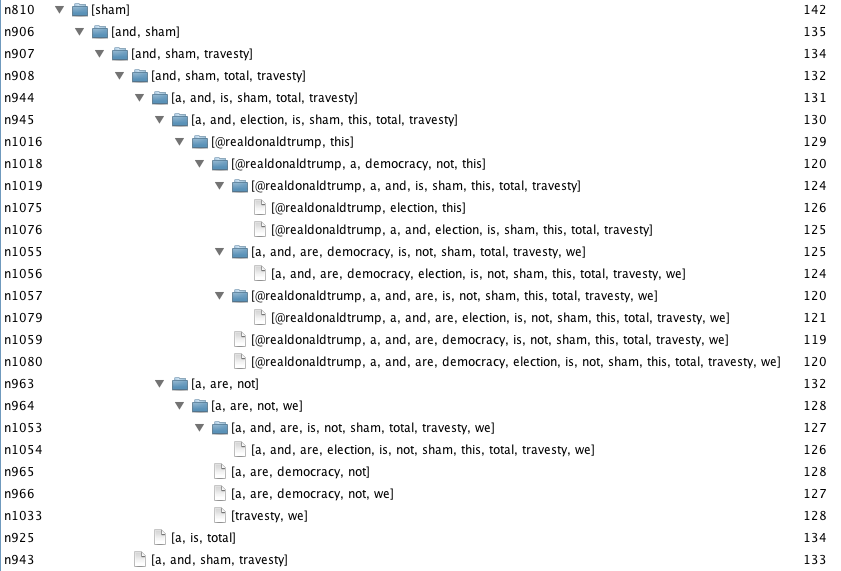
\includegraphics{clustering/hierarchy_sham.png}
}
\caption{The hierarchy of itemsets in the cluster pertaining to the ``sham and travesty'' tweet}
%\caption{Itemsets from the ``sham and travesty'' tweet and how they are clustered together}
\label{fig:hierSham}
\end{figure}
\end{landscape}


\begin{landscape}
\begin{figure}
\begin{tabular}{p{0.8cm}p{13.9cm}p{2cm}}
Id & Itemset &  Support\\ \hline
\end{tabular}
\scalebox{0.7}{
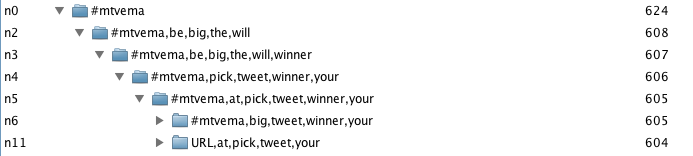
\includegraphics{clustering/ema/general.png}
}
\scalebox{0.7}{
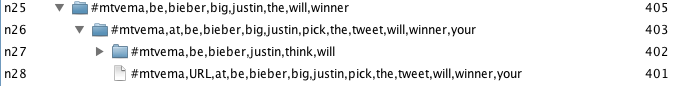
\includegraphics{clustering/ema/bieber2.png}
}
\scalebox{0.7}{
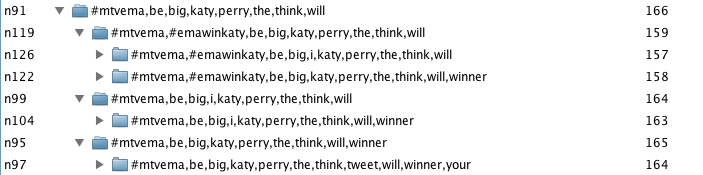
\includegraphics{clustering/ema/katy.png}
}
\scalebox{0.7}{
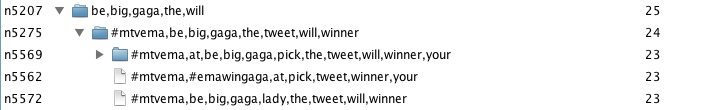
\includegraphics{clustering/ema/gaga.png}
}

\caption{Several clusters for itemsets pertaining to the MTV Europe Music Awards votes} %, one for votes supporting each artist}
%\caption{Itemsets from the ``sham and travesty'' tweet and how they are clustered together}
\label{fig:hierEma}
\end{figure}
\end{landscape}

\subsection{Bounding Space and Time Requirements}
Algorithm~\ref{algo:alliance} requires
keeping \emph{distinct} itemsets 
and their postings lists
%some of the results of LCM 
in memory,
so that the similarity between a \emph{closed} itemset and %\emph{distinct}
all the previously generated \emph{distinct} ones
can be efficiently calculated. 
This is an overhead that the original LCM does not incur, 
but it is not a large overhead;
due to the limited number of \emph{closed} itemsets, % \emph{distinct}
the memory requirements does not exceed 6 GB
for mining hour long epochs using 
a Java implementation that uses a lot of objects. % of RAM
%select args, count(*), avg(value), stddev(value)  from perf_mon where args like '%4wk%1hr%ULBuff%' and key='MemoryMBUsed' group by args;
However, it is possible to use less memory
and also bound the memory requirement by 
%keeping
%only a limited number of itemsets in memory.
setting a hard limit on the number of itemsets kept in memory.

The number of positions between an itemset
and a clustering candidate is 1973.11 on average,
with a standard deviation of 1443.64. 
The large standard deviation indicates that
candidates are either found close to the itemset
(less than 500 positions behind),
or in a position that is several thousands 
of itemsets behind.
According to our observation that itemsets 
from one topic are generated close to each other, 
when the total ordering is descending in items frequency,
we limit the mining results kept in memory 
to the last 1000  itemsets and their postings lists. %\emph{distinct}
%then itemsets whose candidates are so many itemsets between 
This sets a bound on the memory requirement,
as well as the runtime which is 
% number of
dominated by the
similarity calculations. % will be bound by the
Without limiting
the number of itemsets kept in memory,
the runtime 
for filtering and clustering hour long epochs %the memory of about 1 GB 
at $\kappa = 0.25$  
is 5.2 seconds on average.
%select args, count(*), avg(value), stddev(value)  from perf_mon where args like '%4wk%1hr%ULBuff%' and key='CPUMillisFilter' group by args;
This is reduced to less than 1 second
if only the last 1000 results from LCM 
are kept in memory. 
More detailed discussion of the runtime performance
of the algorithm is given in section~\ref{sec:effic}.
The \emph{quality} of the \emph{strongly closed itemsets} 
%clusters
produced with that limit in place
is investigated in section~\ref{sec:effectiveness}.

%merging with it
% select args, count(*), avg(value), stddev(value)  from perf_mon where args like '%4wk%1hr%ULBuff%' and key='bufferSizeNeeded4CandidateMean' group by args;
%[/home/yaboulna/fim_out/lcm_closed_cikm/4wk+1wk_ngram5-relsupp1_oct-nov-dec/, /home/yaboulna/fim_out/lcm_closed_cikm/1hr+30min_ngram5-relsupp10_11032233-11151120_graph/, ULBuff_Canddist_LowCos_conf0.25,  ITEMSET_SIMILARITY_COSINE_GOOD_THRESHOLD=0.5 ITEMSET_SIMILARITY_PROMISING_THRESHOLD=0.0 ITEMSET_SIMILARITY_PPJOIN_MIN_LENGTH=3 ITEMSET_SIMILARITY_BAD_THRESHOLD=0.1 CONFIDENCE_HIGH_THRESHOLD=0.25] |   555 | 1973.11206069111 | 240.226242426062

%select args, count(*), avg(value*value), stddev(value*value)  from perf_mon where args like '%4wk%1hr%ULBuff%' and key='bufferSizeNeeded4CandidateStddev' group by args;
                                                                                                                                                                                                      %args                                                                                                                                                                                                       | count |       avg        |      stddev      
%-----------------------------------------------------------------------------------------------------------------------------------------------------------------------------------------------------------------------------------------------------------------------------------------------------------------------------------------------------------------------------------------------------------------+-------+------------------+------------------
 %[/home/yaboulna/fim_out/lcm_closed_cikm/4wk+1wk_ngram5-relsupp1_oct-nov-dec/, /home/yaboulna/fim_out/lcm_closed_cikm/1hr+30min_ngram5-relsupp10_11032233-11151120_graph/, ULBuff_Canddist_LowCos_conf0.25,  ITEMSET_SIMILARITY_COSINE_GOOD_THRESHOLD=0.5 ITEMSET_SIMILARITY_PROMISING_THRESHOLD=0.0 ITEMSET_SIMILARITY_PPJOIN_MIN_LENGTH=3 ITEMSET_SIMILARITY_BAD_THRESHOLD=0.1 CONFIDENCE_HIGH_THRESHOLD=0.25] |   555 | 2084100.38184268 | 413072.078653635
%sqrt(2084100.38184268 ) =1443.64136192



% warning! --> diff_romney-obama_sel_ULBuff_Canddist_conf0.25_3600_-sel_NoPerfMon_Graph_conf0.25_Buff1000_3600_1352260800_supp37
%wc -l diff_romney-obama_sel_ULBuff_Canddist_conf0.25_3600_-sel_NoPerfMon_Graph_conf0.25_Buff1000_3600_1352* | less -NS
%556   701 total

%wc -l diff_NO-KEYWORDS_sel_ULBuff_Canddist_conf0.25_3600_-sel_NoPerfMon_Graph_conf0.25_Buff1000_3600_* | less -Ns
%556  162232 total


\section{Temporal Ranking}
\label{sec:rank}

%A General Measure of Rule Interestingness
%Szymon Jaroszewicz and Dan A. Simovici
%University of Massachusetts at Boston
We now propose a ranking function that scores itemsets 
%according to their temporal novelty, 
according to their novelty,
such that the ordered list of itemsets 
can be presented to a user as a summary of 
what is happening on Twitter in the mined epoch.
The ranks can also be used as weights for itemsets when
used by other system components, 
such as a search component that uses itemsets for query expansion.

We measure temporal novelty compared to %between the mined epoch %is measured 
a longer period of time 
leading up to the mined epoch
--~a background model.
%that is not far in the past.
%in the recent past
%This can be done using cascade methods (Azin's paper)
A good indicator of novelty is the pointwise Kullback-Leibler Divergence (KLD)
between an itemset's probability in the current epoch and in the background model.
The KLD of the probability of an itemset, $s_i$, in the background
model, $Q$, from the current epoch's model, $P$, can be considered as
the Information Gain, IG: 
\begin{align}IG(P(s_i),Q(s_i))  &= - (H(P(s_i)) - H(P(s_i),Q(s_i))) \notag\\ &= \sum{P(s_i) \log{P(s_i)}} - \sum{P(s_i) \log{Q(s_i)}} \notag\\ &= KLD(P(s_i)||Q(s_i))\end{align}
This interprets the KLD of an itemset's probability as the number of extra bits
in the representation of the itemset
used by an encoding based on Q as compared to the number of bits
used by an encoding based on P; 
hence, the information gain in moving from a prior distribution to 
a posterior distribution.

To calculate the collective IG of itemsets in a \emph{strongly closed itemset},
we have to take into account that the itemsets of the cluster are not independent. 
For simplicity we will consider only the pairwise dependence between 
every itemset and the smallest common subset.
%when calculating the IG of the whole cluster.
The joint probability of the smallest common subset, $s_{min}$,
%occurs and any itemset in the 
and any itemset in the cluster, $s_{j}$, is basically the probability of the itemset $s_{j}$,
since $s_{min} \subset s_{j}$. % is its subsets. 
In other words, the probability of $s_{min}$ conditioned
on any itemset $s_{j}$ in the cluster is 1,
and there is no information in the occurrence
of $s_{min}$ given that $s_{j}$ occurred.
%Therefore,  
%Alternatively, this can be interpreted 
An alternative interpretation is that
there is a shared component in the IG of all itemsets in the cluster,
%information from any two itemsets in the cluster %IG of
which is the IG of $s_{min}$.
%Consider that probabilities of itemsets in the cluster
%are conditioned on the probability of $s_{min}$;
%$prob(s_j) = prob(s_{min})\,prob(s_j|s_{min})$.
%It is easy to see that IG(P(s_j)) = P(s_j|s_{min}) IG(P(s_min),Q(s_{min})) + P(s_{min})....
%In that case, 
%comes from the IG of $s_{min}$; 
%if $P(s_{min})$ were used in the creation of an encoding 
%that is otherwise base on Q, 
%for itemsets in the cluster that is based on 
%then the number of extra bits used for encoding each itemset  in the cluster %$s_{j}$
%would be less than the number of extra bits used 
%in an encoding that is completely based on Q.
%if we add the IG of all of the itemsets in the cluster
%we will be adding the IG of $s_{min}$
%we will be adding the com
%This is 
Hence, the IG of an itemset cluster,
$r=\{s_{i_1},..,s_{i_m}\}$, 
can be approximated as the IG of its smallest subset, $s_{min}$,
plus the IG of each itemset in the cluster conditioned on $s_{min}$:
\begin{align}
IG(P(s_{i_1},...s_{i_m}),Q(s_{i_1},...s_{i_m})) &= IG(P(s_{min}), Q(s_{min})) \notag \\
&+ \sum_{j = i_1..i_m}{IG(P(s_j|s_{min}), Q(s_j|s_{min}))}
\end{align} 
This formula avoids implicitly adding the information gain from $s_{min}$
multiple times to the total information gain. %with the add
%It neglects the overlap between itemsets,
%but 
%it provides an approximation that is good enough
%for ranking itemset clusters 
%as we will see in section~\ref{sec:effectiveness}.
%Several other ranking formulae were tried
%and this one give`s the best results.
%The formula above 
It can be used for ranking clusters,
but it will favour larger clusters.
We normalize by the size of the cluster, giving our final ranking formula for
strongly closed itemsets:
\begin{equation}\label{eq:avgIG}score(r) = IG(P(s_{min}), Q(s_{min})) + \frac{ \sum_{ j = i_1..i_m } { IG(P(s_j|s_{min}), Q(s_j|s_{min})) } } { m } \end{equation}
%\overline{IG}

In this thesis, the background model we use for each day is the results of mining the 4 weeks
before it, using a \emph{minimum support} value of 1 occurrence.
Mining the background model at such a low support increases the number of
produced itemsets, which is desirable for a background model.
All probability estimates are smoothed by add-one smoothing. 


% ==========================================
% C H A P T E R     5
% ==========================================


\chapter{Evaluation}
\label{sec:empirical}

In this chapter we analyze the performance of the methods proposed by applying
them to the mining results of all one-hour long epochs in the Twitter dataset.
We evaluate their efficiency in reducing the number of mined itemsets in section~\ref{sec:effic},
and we assess their effectiveness for choosing a high quality synopsis in section~\ref{sec:effectiveness}. %of the filtering
The experiments were run using a single threaded Java implementation of
algorithm \ref{algo:alliance}, % and the LCM implementation provided by Uno et al. on their website\footnote{}.
%The experiments were 
running on a 1.4 GHz processor with 2 MB of cache.


\section{Efficiency}
\label{sec:effic}
%\label{sec:bounding}

We evaluate the efficiency of our proposed filtering and clustering methods 
in terms of the number of itemsets before and after their application,
and the runtime overhead they add on top of the runtime of the LCM algorithm.
Using variable length N-grams as items, 
the average number of itemsets mined from an hour-long epoch is
2,439.17 closed itemsets of length 2 or more after flattening;
that is, excluding itemsets that are merely a frequent unigram.
We start by analyzing the reduction in this number at different values
of the distinctiveness threshold, $\kappa$.

%The number of length 2 or more maximal itemsets is 1831.92,
%which we provide just as a reference to the result of a basic way of filtering.

Figure \ref{fig:kappa} show the effect of varying $\kappa$ on the mean number
of \emph{distinct} and \emph{strongly closed} itemsets.
The number of \emph{distinct} itemsets drops as the distinctiveness threshold
increases.
On the other hand, the number of \emph{strongly closed} clusters formed increases
as the similarity/indistinctiveness threshold (taken as $1 - \kappa$) decreases.
The dashed line shows that the number of unclustered distinct itemsets reaches
zero at $\kappa=0.5$, explaining why the number of clusters changes very
slightly after that. 
We use $\kappa = 0.25$ in this thesis, %the remainder of the paper,
which is an arbitrary choice based on the definition not the data.
The average number of \emph{strongly closed} itemsets mined from one-hour epochs at this value of
$\kappa$ is 139.1, which is about 5.7\% of the number of closed itemsets of length 2 or more.
%before filtering and clustering. %of closed itemsets.
If we also include unclustered \emph{distinct} itemsets in the synopses, 
their average size increases to 224.49 itemsets per hour long epoch. % on average.



%We now 
Figure \ref{fig:lcmvsfpzhu} shows the total runtime of the LCM algorithm plus
filtering based on the distinct condition and clustering into strong closed
itemsets at different epoch spans.
The runtime of LCM alone is also plotted for reference.
We also plot the performance of another frequent itemset mining algorithm,
FP-Zhu~\cite{grahne2004reducing}, which was the runner up at
FIMI 2004~\cite{DBLP:conf/fimi/2004}.
We include it to show that our extensions do not degrade the performance of
LCM even in the context of competitions.
The y-Axis is in logarithmic scale to keep the scale of the plot suitable for
seeing slight differences.
The output of LCM is the input to the filtering and clustering step,
so it is affected by the number of closed itemsets produced.
Recall that the number of itemsets from epochs of span 
%one hour or more is constant,
less than an hour is higher than that from epoch of span
one hour or more. %(which is constant at the same minimum support threshold).
This explains why it takes slightly longer time for clustering results from
the 15-minute epoch and then takes a constant time for epochs of a longer span. 

%Recall that the number of itemsets from epochs of span 
%less than an hour is higher

\begin{figure}
\centering
\scalebox{0.75}{
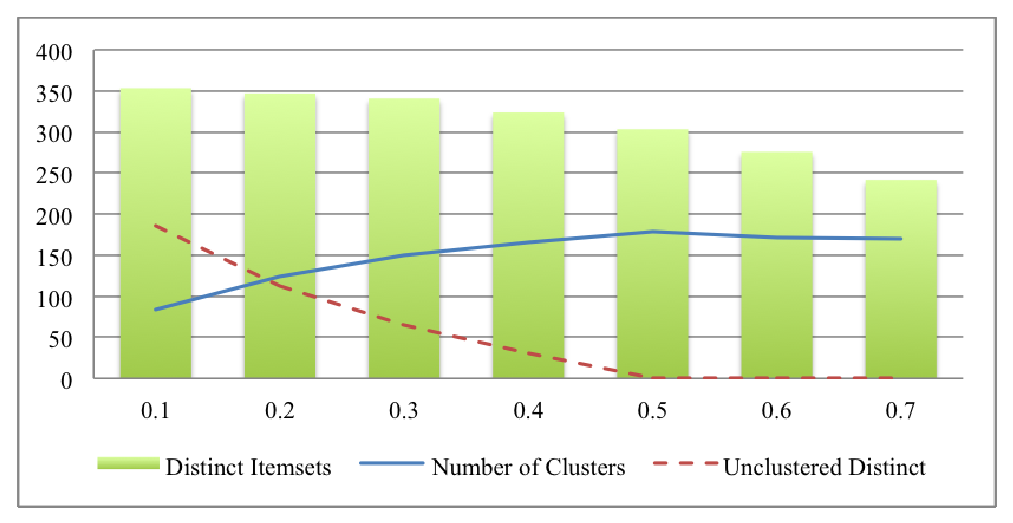
\includegraphics{kappa_effect.eps}
}
\caption{The number of different types of itemsets at different values of $\kappa$, the distinctiveness threshold. The value of $\kappa$ used in this thesis is 0.25, midway between 0 and 0.5 when all distinct itemsets are clustered,
but it was determined according to the definition.}
%The similarity threshold for clustering is taken to be $(1 - \kappa).$}
%Effect of changing  on mining results }
\label{fig:kappa}
\end{figure}

\begin{figure}
\centering
\scalebox{0.8}{
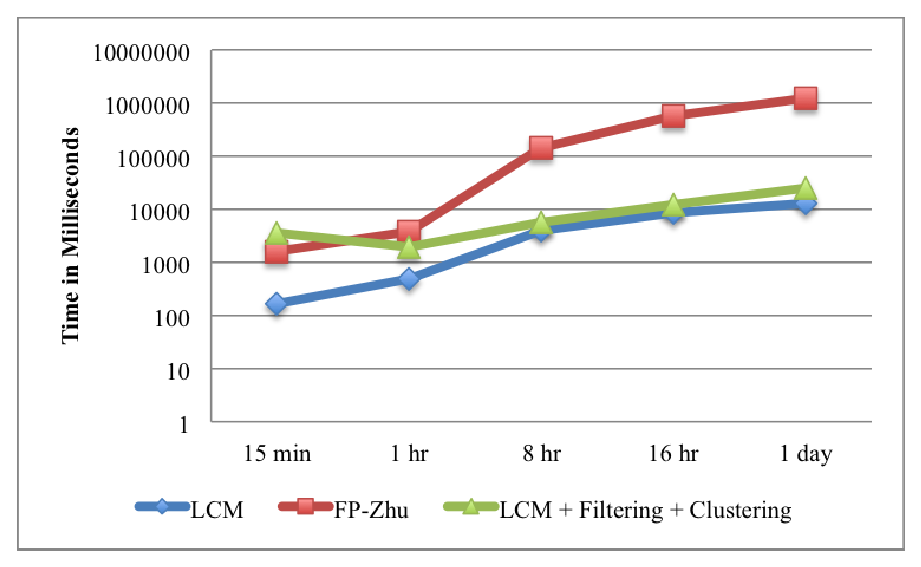
\includegraphics{runtime_lcm-lcm+filter-fpzhu_seconds.eps}
}
\caption{Runtime, at different epoch spans, of the LCM algorithm with and without the filtering and clustering extensions as well as of another efficient frequent itemset mining algorithm. Our extensions do not degrade the efficiency of the LCM algorithm.}
\label{fig:lcmvsfpzhu}
\end{figure}

\section{Effectiveness}
\label{sec:effectiveness}
We now show examples of the synopses produced by ranking
the \emph{strongly closed} itemsets as discussed in section~\ref{sec:rank}.
The examples will serve as our assessment of the quality of 
the synopses. 
We make an effort to choose epochs from time periods when 
%important events were known to happen
%important happenings were 
%known happenings were being talked about. 
it is known what people should be talking about. 
In section~\ref{sec:electionsday}, 
we show how the 2012 US presidential elections day is summarized by our methods. %hour-by-hour
We also compare our summary to the one produced by a state of the art algorithm,
which generates better quality summaries than other summarization algorithms based on itemsets~\cite{mampaey2011tell}. %my the MTV algorithm
In section~\ref{sec:gtrends},
we investigate the synopses of hours selected by the aid of Google Trends\footnote{\url{http://www.google.ca/trends}},
assessing which popular queries were or were not reflected in our synopses.

\subsection{U.S. Presidential Elections Day}
\label{sec:electionsday}
In this section, we focus on the 
2012 US presidential elections day, November $6^{th}$.
We compare the quality of the synopsis of the day created by
our proposed methods to the quality of the synopsis created by
mining the top itemsets with the MTV algorithm~\cite{mampaey2011tell} 
(according to a maximum entropy model).
The synopsis should be suitable for giving 
a user an overview of what people were Tweeting about at %understanding of 
different times of the day. %on the 2012 US presidential election

Table \ref{table:nov6} shows the top 3 \emph{strongly closed} itemsets
from one-hour epochs on the elections day, 
%starting either at the hour or the half-hour mark. 
using a half-hour time step.
The itemsets shown are the first appearances of the most interesting itemsets;
that is, an hour is shown only if its top 3 feature novel interesting itemsets\footnote{The top 50 itemsets in the hours from 5 AM on the 6th till 
almost 9 AM on the 7th are available for download at \url{http://plg.uwaterloo.ca/~yaboulna/thesis_results/twitter_synopses/elections-day_nov6-0500_nov7-0850_top50-strongly-closed.txt}}.
The first column is the beginning of the hour, EST time.
The second column is the top itemsets, 
reordered and punctuated to be meaningful phrases 
by looking at a few tweets from the postings list of each itemset.
The third column is a commentary to explain the itemsets,
also composed constructed according to tweets in the postings lists.
The fourth column is the rank of an equivalent itemset 
in the top 30 itemsets mined by the MTV algorithm, if one exists.
%In table \ref{table:nov6}, 

We can see how the events of the US presidential
elections  unwind from ``get out and vote'' to the projections and debates,
all the way to the ``acceptance speech''.
Early in the day, people were excited 
and congratulating each other for being on the elections day. 
The excitement  continues for one more hour, 
with some people taking it too far by sending pictures of their ballots.
Itemsets about the elections stop occupying the top 3 ranks until the evening. 
During the day, the top 3 ranks were occupied by itemsets about UEFA Champions football matches
(with timely updates of their scores), and about TV shows. 
We include the top 3 itemsets of 3 PM as an example.
In the evening, the elections heat up 
and events about it keep occupying top positions
in all epochs.
At 10 PM all the top 5 were relevant and very interesting 
that we decided to include an extra two itemsets in the example 
(we do this for MTV as well, in the hour of the acceptance speech).
Shortly after the results of the elections became clear, news that
Marijuana and same sex marriage were legalized in some states
occupy the top rank.
This exemplifies the power of social media as a collaborative filter,
selecting the news of greatest importance to social media users.
The user centric definition of importance is also evident in the attention
given to the ``lady with a flag in her hair'' appearing on TV behind Obama 
during the acceptance speech. 

%\addtolength{\voffset}{-3cm}
%\newgeometry{top=1cm,bottom=1cm}
%\changepage{1cm}

\begin{table}
%\vspace{-3cm}
\thisfloatpagestyle{empty}
%\thispagestyle{empty}
\begin{center}
\footnotesize
\def\arraystretch{1.1}
\begin{tabular}{|p{1cm}|p{6cm}|p{8cm}|c|}
\hline
\textbf{Time} & \textbf{Itemset} & \textbf{Explanation} & \textbf{MTV} \\ \hline
\multirow{3}{*}{\texttt{08:30}}
& \em get out and vote & Encouraging participation & 17 \\ \cline{2-4}
& \em happy elections day & Congratulations & 27 \\ \cline{2 - 4}
& \em it's elections day & Excitement  & - \\ \hline

\multirow{3}{*}{\texttt{09:30}}
& \em if romney wins & People reflecting about the different possible results & - \\ \cline{2 - 4} %dreading the thought (according
& \em of your ballot & Telling people to stop sending pictures of ballots & - \\ \cline{2-4}
& \em in line to vote & Tweeting while standing in line  & 28 \\ \hline

\multirow{3}{*}{\texttt{15:00}}
& \em Borussia Dortmund Real Madrid 2 & Score update of UEFA football match & 17 \\ \cline{2 - 4}
& \em incroyable talent & France's version of the Got Talent TV show & - \\ \cline{2-4}
& \em City Ajax 2 & Score of Manchester City vs Ajax  & - \\ \hline

\multirow{3}{*}{\texttt{19:30}}
& \em Linda  McMahon		&  Linda McMahon loses CT senate race & - \\ \cline{2 - 4}
& \em Florida is so ... & tight or close; the number of votes  & - \\ \cline{2-4}
& \em Romney is winning & Speculations about the results  & - \\ \hline %He did take the lead for a while


\multirow{3}{*}{\texttt{20:00}}
& \em New Hampshire &  Obama won in NH & 9 \\ \cline{2 - 4}
& \em Obama to win / is winning & Two itemsets speculating  & - \\ \cline{2-4}
& \em too close to call & The results are still not clear & 22 \\ \hline


\multirow{3}{*}{\texttt{21:00}}
& \em Ohio and Florida &  Obama won in 2 more states & - \\ \cline{2 - 4}
& \em Sarah Palin & Sarah Palin appears on Fox news  & - \\ \cline{2-4} %(uh oh!)
& \em concession speech & Todd Akin's concession speech & - \\ \hline


\multirow{5}{*}{\texttt{22:00}} 
& \em The electoral college &  Republicans complaining about the voting system  & 9 \\ \cline{2 - 4}
& \em President of the United States & Barack Obama is the 44th president of the USA   & 8 \\ \cline{2-4} %(uh oh!)
& \em who voted for & People turning against each other & - \\ \cline{2-4} % 
& \em once you go black you never go [back] & A popular culture reference & 15 \\ \cline{2-4} %(uh oh!)
& \em my president is black & Americans proud about the equality of opportunities & - \\ \hline % 

\multirow{3}{*}{\texttt{22:30} }
& \em @realdonaldtrump this elections (see table \ref{table:mtv} for the rest of the tweet) 		& One of Donald Trump's famous melt down tweets. This cluster merges 26 \emph{distinct} itemsets. & 1  \\ \cline{2-4}
& \em concede to & The losing candidate has to concede  & - \\ \cline{2-4} %(uh oh!)
& \em Obama won. I ... & People's reactions to the results & - \\ \hline % 

\multirow{3}{*}{\texttt{23:00} }
& \em same sex marriage	& Some states legalized same sex marriage & 27  \\ \cline{2-4}
& \em for recreational use & Colorado legalized Marijuana for recreational use   & 21 \\ \cline{2-4} %(uh oh!)
& \em acceptance speech & People anticipating the speech & 26 \\ \hline % 

\multirow{3}{*}{\texttt{00:30} }
& \em Delivered, sealed, signed & Stevie Wonder's song used in Obama's campaigns & 10  \\ \cline{2-4}
& \em The best is yet to come & Quote from Obama's acceptance speech  & 2 \\ \cline{2-4} %(uh oh!)
& \em with the flag in her [hair]	&  During the speech, attention on social media goes to a woman appearing behind Obama on TV! & 14 \\ \hline %  \cline{2-3}

\multirow{3}{*}{\texttt{01:00} }
& \em Four more years & Barack Obama's tweet; the most retweeted in 2012 %\footnote{\url{http://ca.news.yahoo.com/blogs/ticket/obama-wins-twitter-election-most-rt-d-tweet-174452713--election.html}} 
& 20  \\  \cline{2-4} %(now)
& \em @paulmyers47: spots & Pyramidal marketing; people retweet to make money & 12 \\  \cline{2-4}
& \em President Barack Obama & News headlines about the speech uses the formal title & - \\\hline
											
\end{tabular}
\end{center}
\vspace{-5mm}
\caption{Top 3 \emph{strongly closed} itemsets for hours in US presidential elections day} %  showing how the day unwound (or 5)
 \label{table:nov6}
\end{table}

%\restoregeometry
%\addtolength{\voffset}{3cm}

 \begin{table}
 \begin{center}
\footnotesize
\def\arraystretch{1.1}
\begin{tabular}{|p{1cm}|p{13cm}|c|c|} %p{9cm}|p{6cm}|}

\hline
\textbf{Time} & \textbf{Itemset} & \multicolumn{2}{c|}{\textbf{Ranks}} \\ %MTV & SC\\
%\hline
\hline
\multirow{3}{*}{\texttt{19:00}} &
 \emph{A partir de que idade voc\^{e} considera algu\'{e}m velho? (Portuguese for ``From what age do you consider someone old?'')}  & 1 & 22 \\ \cline{2-4} %
& \emph{A qu\'{e} edad consideras que alguien es viejo? (Spanish for the same question above; we do not know what started this meme)} & 4 & 10 \\ \cline{2-4}
& \emph{We'll find out if it's true. America went black, will it go back?} & 9 & 24 \\ \hline

\multirow{3}{*}{\texttt{20:30}} &
\emph{Obama rhymes with Ohana. Ohana means family \& family means nobody gets left behind. Mitt rhymes with shit.} 
& 3 & 3 \\\cline{2-4}
& \emph{New Hampshire}	& 9 & 1 \\ \cline{2-4}
& \emph{\#IamSickOf} & 10 & - \\ \hline

\multirow{3}{*}{\texttt{21:00}} 
& \emph{We're all in this together. That's how we campaigned, and that's who we are. Thank you. -bo} & 1 & 22 \\ \cline{2-4} %266031109979131904
& \emph{@barackobama This happened because of you, thank you. } & 4 & 20 \\ \cline{2-4}
& \emph{@barackobama Four more years URL} & 6 & 6 \\ \hline

\multirow{3}{*}{\texttt{22:00}} 
& \emph{@realDonaldTrump: We can't let this happen. We should march on Washington and stop this travesty. Our nation is totally divided!} & 5 & 44  \\ \cline{2-4}
& \emph{President of the United States} & 8 & 2  \\\cline{2-4} % 266035509162303492
& \emph{@realDonaldTrump: The electoral college is a disaster for a democracy.} & 9 & 1
%266037143628038144
\\\hline %


\multirow{3}{*}{\texttt{22:30}} &
\emph{@realDonaldTrump: This election is a total sham and a travesty. We are not a democracy!} & 1 &1  \\\cline{2-4} % 266035509162303492
& \emph{@realDonaldTrump: Our country is now in serious and unprecedented trouble...like never before.} & 3 & 24 \\ \cline{2-4}
%266037143628038144
& \emph{@realDonaldTrump: He lost the popular vote by a lot and won the election. We should have a revolution in this country!} & 5 & 31 \\\hline %

\multirow{3}{*}{\texttt{23:00}}
& \emph{@realDonaldTrump: Lets fight like hell and stop this great \& disgusting injustice! The world is laughing at us.} 
& 4 & 48
\\ \cline{2-4}
& \emph{@realDonaldTrump: House of Representatives shouldn't give anything to Obama unless he terminates Obamacare.} 
& 6 & 15 \\\cline{2-4}
% 266040877552656385
& \emph{@adamlevine: That's what happens when you fu** with Sesame Street} 
& 8 & 18 \\\hline 


\multirow{3}{*}{\texttt{00:30}} &
\emph{The best is yet to come} & 2 & 2  \\\cline{2-4} % 266035509162303492
& \emph{Michelle, I have never loved you more} & 5 & 12 \\ \cline{2-4}
%266037143628038144
& \emph{We are an American Family, and we rise ...} & 8 & 20 \\ \cline{2-4}
%266037143628038144
& \emph{Delivered, sealed, signed, I'm yours} & 10 & 1 
\\\hline %


\end{tabular}
\end{center}
\caption{The most interesting itemsets out of the top 10 picked by the MTV algorithm for hours in US presidential elections day. The actual rank given to each itemset by MTV is in column 3 and the rank of its equivalent \emph{strongly closed} itemset is in column 4. Interesting itemsets in the top 10 itemsets selected by MTV are all included in our synposes.}
%MTV tends to pick complete Tweets with lots of retweets.}
 \label{table:mtv}
\end{table}


%The top 3 itemset mined by the MTV algorithm~\cite{mampaey2011tell}  are shown in table \ref{table:mtv}.
% we show the top 3 itemsets picked by the MTV algorithm~\cite{mampaey2011tell} for the same epochs and support.
%for one-hour epochs. 
%
The top 3 itemset mined by the MTV algorithm~\cite{mampaey2011tell}
are usually itemsets from Tweets sent by
services reporting users' scores in games, 
or the number of new followers each user got.
However, the top 10 itemsets usually contain
% topically relevant itemsets.
interesting itemsets\footnote{The top 30 itemsets in the hours from 5 AM on the 6th till 
5 AM on the 7th are available for download at \url{http://plg.uwaterloo.ca/~yaboulna/thesis_results/twitter_synopses/elections-day_nov6-0500_nov7-0500_top30-MTV.txt}}.
Therefore, in table \ref{table:mtv} we show itemsets 
%relevant to the U.S. presidential elections 
that we find interesting
from MTV's top 10,
assuming that the itemsets from Tweets sent by automatic services
can be filtered out by another dedicated filter.
The actual rank in which the itemset appeared 
is shown in column 3, 
and the rank in which it appears among \emph{strongly closed}
itemsets is shown in column 4.
%prepended to it.  %the itemset.
We show only hours in which the top 10 itemsets contain 
novel interesting itemsets. 
The itemsets chosen by MTV tend to be complete Tweets 
which were retweeted by many users,
thus we omit the explanation column for brevity.
%For brevity, we truncate itemsets that are complete tweets and append the tweet id for reference.
% 
%It is noteworthy that tweets that spark a conversation contribute multiple redundant itemsets, and several of them are ranked high.
% (Nov. 6 22:00). This stresses the importance of clustering.
%The harm from redundancy is amplified by the low values of $k$ that has to be used. 
% to attain an acceptable runtime.
The input to the algorithm was transactions made up of N-grams up to 5 terms long. 
%which 
This helped the algorithm converge faster since the distribution is flatter. 
The use of N-grams also overcomes the dominance of language constructs, 
which are ranked high in all hours if unigrams are used. % instead.



All the topically relevant itemsets chosen by MTV are present in 
the top 50 \emph{strongly closed} itemsets
~--~most of them are in the top 30.
We do not know if all the top ranked \emph{strongly closed} itemsets 
%are also in picked up at a relatively high rank
would also be picked by MTV if we use it to mine more itemsets.
%since 
The space and time requirements of MTV
becomes prohibitively large when the number
of itemsets requested is increased,
as it takes more than an hour to mine 
the top 50 itemset from an hour long epoch.
%and
%we did not have time to get its results for all epochs at $k > 30$.
% beyond 
At $k > 100$ the MTV algorithm fails because of a memory error, 
even though it was being run on a machine with 256 GB of RAM,
with no limit on its resource consumption.
%At $k = 30$ the algorithm was left running for days and it finished 
%mining only a few hour long epochs. 
%Therefore, we conclude from the comparison 
%that our methods can  efficient
%that MTV is not superior well rooted theoretically
The runtime performance at $k \le 100$ is plotted in figure~\ref{fig:mtvPerf}.
The small value of $k$ that has to be used 
makes MTV inadequate for mining social media,
where the high volume of posts 
and the variety of topics users talk about
is likely to result in more itemsets than 
what MTV would pick as the top $k$.
On the other hand, \emph{strongly closed} itemsets
are efficiently mined and are not restricted to a predefined number.
%The quality of the results is comparable, but
%The efficiency does not cquality of the results of 

 
\begin{figure}
\centering
\scalebox{0.9}{
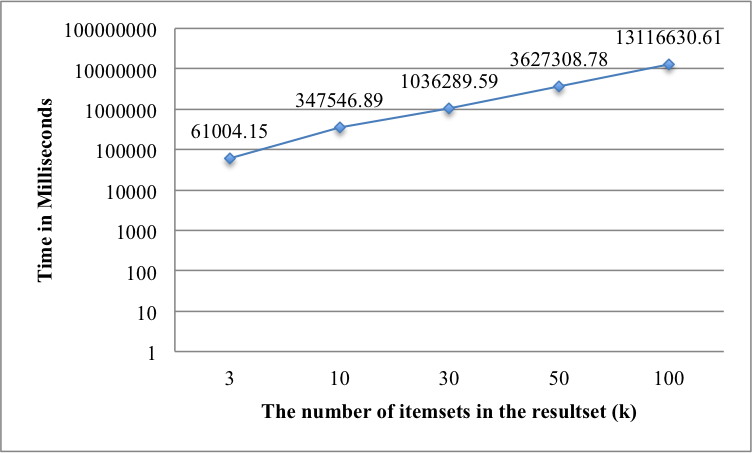
\includegraphics{mtv_runtime.png}
}
\caption{Runtime of mining an hour long epoch using the MTV algorithm~\cite{mampaey2011tell} at different resultset sizes (top k). The runtime increases exponentially with increasing values of k.} %, and is not short to start with
\label{fig:mtvPerf}
\end{figure}

\subsection{Google Trends}
\label{sec:gtrends}
Google Trends is a freely available service provided by Google.
It analyzes queries submitted to the Google search engine by millions of users worldwide,
and it can be used to know the most popular queries %what people 
for different geographies\footnote{\url{http://www.google.ca/trends/}}.
%are searching for.
It can also be used to compute
trends of user specified queries
over time\footnote{\url{https://support.google.com/trends/answer/87276?hl=en}}.
Queries that are named entities according to Google's Knowledge Graph\footnote{\url{http://www.google.com/insidesearch/features/search/knowledge.html}} 
are automatically tracked 
and aggregated by category
into Top Charts\footnote{\url{http://www.google.ca/trends/topcharts}}~--~
lists of real-world people, places and things ranked in order of search volume 
%during different intervals of time. 
during user specified intervals of time\footnote{\url{https://support.google.com/trends/answer/3076011?hl=en}}.
We use the Top Charts of November 2012 
for the people category\footnote{\url{http://www.google.ca/trends/topcharts\#vm=chart&cid=people&geo=US&date=201211}}
(only available for queries made from the USA)
as an aid for finding out what social media users
are expected to be talking about.
%We use the Top Charts of the following categories:
%people\footnote{http://www.google.ca/trends/topcharts\#vm=chart\&cid=people\&geo=US\&date=201211},
%sports teams\footnote{http://www.google.ca/trends/topcharts\#vm=chart\&cid=sports\_teams\&geo=US\&date=201211},
%soccer teams\footnote{http://www.google.ca/trends/topcharts\#vm=chart\&cid=soccer\_teams\&geo=US\&date=201211} and
%TV shows\footnote{http://www.google.ca/trends/topcharts\#vm=chart\&cid=tv\_shows\&geo=US\&date=201211}.
We observed that named entities that make it to the top 10 chart in the people category %occupying the top positions
are divided into finer groups. %categories, 
The queries about 
people in each group %finer category %strongly correlated in its 
have similar volumes over time, 
%which can be tracked down to real world events.
with peaks at the times of real world events
in which those people in the group took part.
For example, the top two % positions in the \emph{people} category 
%are occupied by the \emph{US politicians} 
most searched for people are
Barack Obama and Mitt Romney.
Figure \ref{fig:trendObamaRomney} is the plot showing the volume of queries about either of them,
as displayed by Google trends\footnote{\url{http://www.google.ca/trends/explore\#q=Barack\%20Obama\%2C\%20Mitt\%20Romney&geo=US&date=11\%2F2012\%201m&cmpt=q}}. 
The two curves in the plot are similar; 
both have peaks at the elections day
and are otherwise flat.
Note that the y-Axis in the figure is scaled\footnote{\url{https://support.google.com/trends/answer/87282?hl=en&ref_topic=13975}} so that the 
maximum volume per day for either of the queries becomes 100 
(to our surprise the curve for ``Barack Obama'' is much lower that that of ``Mitt Romney'',
even though they occupy positions 1 and 2 respectively in the Top Chart).
%According to the observation that
Since entities can be grouped together
%we compare the itemsets found by our  results of
according to the events which made users search for them,
we use the Top Charts
% that are 
%picked by the
%algorithms which enumerate the Top Charts
to know about %as ground truth for
real world events which were of interest to internet users.
We evaluate the use of \emph{strongly closed} itemsets 
as temporal synopses by
investigating the mining results from 
the time periods when these events were happening.
We look for itemsets about
those entities and events in the top 30 \emph{strongly closed} itemset,
and assess which 
of them were or were not reflected in our synopses.
The number of itemsets from each hour is limited to 30 because 
this is a number that can be conveniently displayed as a summary for a human user. 
 
\begin{figure}
\centering
\scalebox{0.5}{
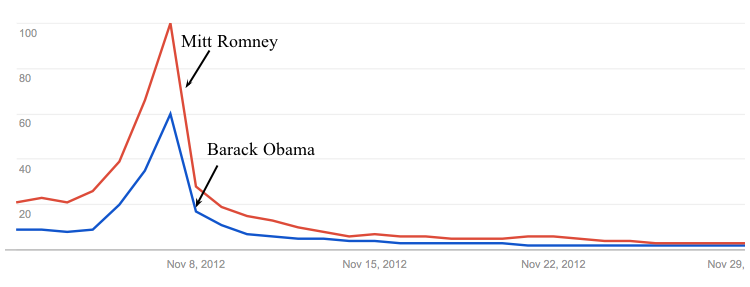
\includegraphics{trends/obama-romney.png}

}
\label{fig:trendObamaRomney}
\caption{Google Trends' volume with time plot for the queries ``Barack Obama'' and ``Mitt Romney'', the top 2 in the Top Chart for the \emph{people} category in November 2012. 
Both curves show a peak of interest at the day of the U.S. presidential elections.}
\end{figure}

\subsubsection{Pop artists and music awards events} 


%http://www.google.ca/trends/explore#q=Justin%20Bieber%2C%20Taylor%20Swift%2C%20Rihanna%2C%20Nicki%20Minaj%2C%20Selena%20Gomez&geo=US&date=11%2F2012%201m&cmpt=q

Pop artists occupy most of the top 10 chart for the \emph{people} category.
Five out of the top 10 are pop artists, and they occupy ranks as high as 3 (Justin Bieber) and 4 (Taylor Swift).
This is due to music awards events, specially
the MTV Europe Music Awards on November 11th\footnote{\url{http://en.wikipedia.org/wiki/2012_MTV_Europe_Music_Awards}} 
and the American Music Awards on November 18th\footnote{\url{http://en.wikipedia.org/wiki/American_Music_Awards_of_2012}}. 
Figure~\ref{fig:trendsPopArtists} shows the query volumes for the artists in the top 10 chart. 
The curves for all of the artists show relatively high volume when those events were happening.

\begin{figure}
\centering
\scalebox{0.5}{
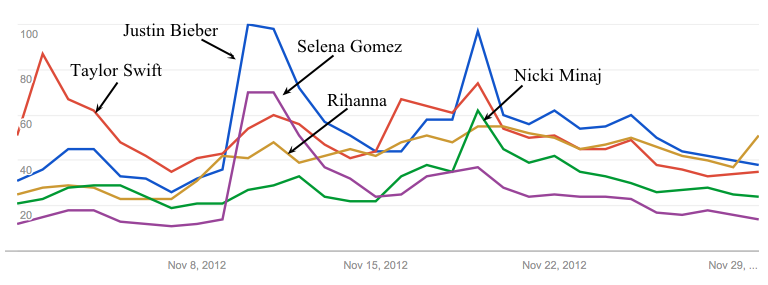
\includegraphics{trends/pop-artists.png}
}
\label{fig:trendsPopArtists}
\caption{Google Trends' volume with time plot for the queries about pop artists in the Top Chart for the \emph{people} category in November 2012. The curves for different artists show similar trends with high search frequency at the times of music awards events.}
\end{figure}



The top 30 \emph{strongly closed} itemsets mined from hours leading to 
% both of the events contain
the MTV Europe Music Awards contain
many itemsets about the events and the artists, 
especially that this event used social media to collect audience votes. 
Voting for the award winner is %MTV Europe Music Awards
a good example of a topic where people have strongly different opinions.
We have shown earlier, in figure~\ref{fig:hierEma},
that such different opinions are all reported as separate \emph{strongly closed} itemsets, 
because clustering in the transaction space avoids forming incohesive clusters. %using the postings lists 
We also note that different  \emph{strongly closed} itemsets from one such topic
can all occupy high ranks.
%For example, the top 3 itemsets of the hour 15:00 on November 9th
%are supporting ``Katy  Perry'', ``Justin Bieber'' and ``Lady Gaga'' respectively.
For example, the top 10 itemsets for the hour starting 9:30 EST on November $11^{th}$
are shown in table~\ref{table:mtvemaTop10}.
The number in parenthesis next to each item is the number of 
itemsets in the cluster which contain this item.
Items in the itemset are sorted by their frequency in this hour, in descending order.
The first itemset in the top 10 reflect the winner, Justin Bieber.
Itemsets about other topics also appear in the top 10; 
there was a football game between Chelsea and Liverpool, and 
November $11^{th}$ is the day World War I ended 
(observed as Remembrance day in the United Kingdom and the Commonwealth of Nations,
% including Australia and Canada
and Veteran's day in the USA).
Several other hours have itemsets supporting different artists in the top 30,
%Almost all of the itemsets about the event are vote itemsets, 
which are all variations of the itemset: \{i, think, ARTIST, NAME, will, be, the, big, winner, tweet, your, pick, at, URL\footnote{\url{http://ema-twittertracker.mtv.com/live/predict.html}}, \#mtvema\}.
%\#emawinARTIST, 

\begin{table}
\centering
\footnotesize
%cut -f 1 sel_June16Defaults_NoLonely_conf0.25_Buff1000_3600_1352647800_supp24 | less -NS
\begin{tabular}{|p{0.5cm}|p{15cm}|}
\hline 
1 & \#emawinbieber(43), \#mtvema(92), URL(31), at(47), be(77), bieber(62), big(81), i(24), justin(62), pick(50), the(62), think(48), tweet(74), will(77), winner(67), your(65)\\ \hline 
2 & \#jonasbrothers(3), \#emawinjoej(4), \#joejonas(3)\\ \hline 
3 & \#emawinbieber(1), \#justinbieber(2)\\ \hline 
4 & \#emawinbieber(2), \#justinbieber(2), \#emavotebieber(4)\\ \hline 
5 & chelsea(2), liverpool(2), vs(3)\\ \hline 
6 & \#staycurrent(3), you(1), @buysocialclout(2), can(1), follow(1), today(1)\\ \hline 
7 & \#emavoteonedirection(1), URL(2), emavoteonedirection(1)\\ \hline 
8 & \#emawinbieber(1), \#justinbieber(2), @justinbieber(2)\\ \hline 
9 & remembrance(2), day(1)\\ \hline 
10 & veteran(2), day(1), s(2)\\ \hline 
\end{tabular}
\label{table:mtvemaTop10}
\caption{Top 10 itemsets in an hour in the morning of the day of MTV Europe Music Awards, 
showing different Strongly Closed itemset clusters voting for different artists }
\end{table}

The American Music Awards (AMAs) did not use social media
to collect votes, so there was not as much posts about it as MTVEMA.
However, itemsets about it still occupied top positions. 
There are several hours where the itemset \{american, music, awards\}
occupied the top rank, but the hour we choose to show as an example does not.
We chose this hour because 
%it is the only one that contains actual 
it contains an itemset that offers
more information than what is contained in other
itemsets from other hours;
itemsets during this event were mainly
names of artists, or the name of the event.
% itemsets usually contain; 
%itemsets are usually either a whole tweet that is indicate that 
The itemsets from this hour, shown in table~\ref{table:amaTop30},
contains an itemset (at position 26) about 
how Justin Bieber appeared with his mother Pattie Mallette\footnote{\url{http://hollywoodlife.com/2012/11/18/justin-bieber-brings-mom-to-amas-without-selena-gomez/\#!1/nokia-jenny-mccarthy/}}
instead of his usual escort Selena Gomez, his ex-girlfriend. 
This is interesting news, 
specially following Justin and Selena's break up
that warranted both of their names a surge in 
their popularity as search queries on November $9^{th}$ and $10^{th}$.
The news of the break up appeared in the top 30 itemsets of different hours on those days.
We include some example tweets randomly selected from the
tweets in the postings lists of the \emph{strongly closed} itemset \{justin, bieber, and, selena, gomez\}.
This shows how including the postings lists in the mining results makes the synopses 
particularly rich, because the actual posts from which they were mined can be easily retrieved: 
%at that time period include shares of news articles such as:
\begin{itemize}
\item \emph{``Justin Bieber and Selena Gomez Break Up http://eonli.ne/SByVNK'' WHAT?!?!?! Is this truee? @justinbieber @selenagomez}'' % https://twitter.com/emeliemcelroy/status/267119732208070656:
%sad comments such as: 
% https://twitter.com/xAnnaVampx/status/267134185767055361
\item \emph{``Justin and Selena broke up? O\_o the awkward moment when he wrote a song about her and another with her name in it...''}
%, and
%some hopeful comments:
%https://twitter.com/katrinaa_xx/status/267118952071712768
\item \emph{``apparently there is a rumor that justin bieber and selena gomez broke up? GO @jessleigh1122 GO!!!!!''}.
%https://twitter.com/katrinaa_xx/status/267118952071712768
%apparently there is a rumor that justin bieber and selena gomez broke up? GO @jessleigh1122 GO!!!!!
\end{itemize}
The itemsets in table~\ref{table:amaTop30}
also include the names of other artists that are not in the Top Chart.  
Liam Payne (rank number 5) is a member of the band One Direction, 
which won several awards that night.
Carly Rae Jepsen (rank number 9) also performed and won an award at the American Music Awards\footnote{\url{http://blog.muchmusic.com/carly-rae-jepsen-wins-at-the-american-music-awards-puts-on-fun-and-flirty-performance/}}.




\begin{table}
\footnotesize
\begin{tabular}{|p{0.5cm}|p{15cm}|}
\hline 
1 & @vinoalan(1), \#vinofollowspree(2)\\ \hline 
2 & vote(2), \#peopleschoice(2), voted(1), retweet(2), @peopleschoice(4), URL(3), for(1), i(1), just(1), to(2), via(3)\\ \hline 
3 & @simoncowell(2), follow(2), me(2), please(2), to(1)\\ \hline 
4 & grinch(2), stole(2), all(3), christmas(2), for(2), haters(3), how(1), is(1), the(5), this(1)\\ \hline 
5 & you(1), @real\_liam\_payne(2), thank(2)\\ \hline 
6 & grinch(3), stole(2), how(1), the(3)\\ \hline 
7 & all(3), amas(1), for(3), is(2), the(4), this(2), watching(2)\\ \hline 
8 & grinch(1), stole(2), christmas(2)\\ \hline 
9 & jepsen(3), carly(1), rae(2)\\ \hline 
10 & dumb(1), dumber(2)\\ \hline 
11 & 3(2), @real\_liam\_payne(2), URL(1), live(1), on(1)\\ \hline 
12 & hi(2), say(1), to(2)\\ \hline 
13 & oz(1), wizard(2), of(2), the(2)\\ \hline 
14 & liam(1), @real\_liam\_payne(1), URL(1), ama(1), live(1), on(2), the(1)\\ \hline 
15 & american(2), awards(2), music(3)\\ \hline 
16 & ama(3), award(3), first(1), night(1), of(3), s(2), the(6), watching(1)\\ \hline 
17 & @simoncowell(1), @real\_liam\_payne(1), call(2), follow(2), me(3), so(2)\\ \hline 
18 & pone(3), triste(2), qu�(1), te(3)\\ \hline 
19 & is(1), on(1), red(1), the(2), wanted(1)\\ \hline 
20 & @simoncowell(1), simon(3), call(1), follow(3), me(2), please(3)\\ \hline 
21 & american(2), awards(1), music(2), the(2)\\ \hline 
22 & carpet(2), red(1)\\ \hline 
23 & oz(1), wizard(3), of(2)\\ \hline 
24 & imessage(2), is(1)\\ \hline 
25 & series(1), survivor(2)\\ \hline 
26 & and(3), justin(2), pattie(2)\\ \hline 
27 & you(4), @real\_liam\_payne(3), URL(1), found(2), i(2), live(1), love(1), on(1)\\ \hline 
28 & \#getglue(2), URL(1)\\ \hline 
29 & \#gameinsight(1), \#android(2), \#androidgames(1), URL(3), android(1)\\ \hline 
30 & \#gameinsight(1), \#android(2), \#androidgames(3)\\ \hline 

\end{tabular}
\label{table:amaTop30}
\caption{Top 30 itemsets from 18:30 EST on the day of American Music Awards (AMAs) showing several mentions of the event, as well as news about Justin Bieber in rank 26.}
\end{table}

%MTVEMA: From 11 / 09 / 12 @ 4:30:00pm EST (1352500200) to 11 / 13 / 12 @ 3:30:00am EST (1352799000)


%yaboulna@hops:~/fim_out/lcm_closed_thesis/1hr+30min_ngram5-relsupp10_oct-nov-dec/sorted14_thesis-formula
%November 18 5PM - EOD: head -n 30 *conf0.25*1353@(28|29|30|31)* | less -NS --> Justin and Pattie (http://hollywoodlife.com/2012/11/18/justin-bieber-brings-mom-to-amas-without-selena-gomez/#!1/nokia-jenny-mccarthy/)  and Let's go Taylor
%head -n 50 *conf0.25*1353@(7|8)* | less -NS ==> replacebiebersongwithcereal
%head -n 100 *conf0.25*135297* | less -NS ==> No bieber no taylor swift

%head -n 30 *conf0.25*1351@(76|77|78|79|8)* | less -NS ==> taylor swift in top 30 at 1351825200 (11 / 01 / 12 @ 10:00:00pm EST), top 50 also in 1351828800 (11 / 01 / 12 @ 11:00:00pm EST) and 1351814400 (11 / 01 / 12 @ 7:00:00pm EST)


\subsubsection{People appearing in the Top Charts but not in the synopses}

Out of the five pop artists appearing in the Top Chart,
as shown in figure~\ref{fig:trendsPopArtists},
the names of only four appeared repeatedly in the top 30 itemsets %artists
of hours in the days of their respective higher search volume.
The name of Rihanna never appeared in any \emph{strongly closed} itemset.
Actually it rarely appeared in any itemset of length 2 or more. 
It is not unusual for an itemset about an artist to be merely his or her name,
%which is just one word in the case of some artists such as Rihanna and Adele
%possibly because users talk about artists using different wordings.
and several artists, like Rihanna, are known by their first name only.
It is impossible for an itemset of length 1 to be \emph{distinct},
since this condition requires that the itemsets be implied
by one of its subsets with high confidence.
Therefore \emph{distinct} and \emph{strongly closed} itemsets
would never capture information in an itemset of length 1.
The same happens with one more of the names in the Top Chart,
Abraham Lincoln. 
During the month of November people were talking on Twitter about 
Lincoln the movie %\footnote{http://www.imdb.com/title/tt0443272/}, 
%not Abraham Lincoln as a 
and this was reflected in mining the term as a closed 1-itemset from 
several hours throughout the month.
However, there were not any closed itemsets longer than 1 item,
and thus there was no mention of Lincoln the movie in the synopses.
This shortcoming can be overcome %would not occur
by settitng a lower support threshold  
so that longer itemsets are mined. 
% for each 
 

Another two celebrities who appear in the top 10 chart 
but not the synopses are Kim Kardashian and Michael Jordan.
The volume of queries about Kim Kardashian is different from other artists,
since she is not a pop music artist and does not participate in music awards events.
For these two celebrities, the volume of queries does not have high peaks, 
and the curve is relatively flat. 
Itemsets mined from Twitter rarely mention either of them. % Kim Kardashian.
Of all itemsets mined from hour long epochs throughout the month of November, 
only 37 closed itemsets contain ``Kim Kardashian'' or ``@kimkardashian'',
and none contain ``Michael Jordan'' or ``@jumpman23'' (his verified username).
%Only 16 of those \emph{distinct}
This means that the number of occurrences of their names is lower than
the support threshold in the all or almost all of the 1,440 overlapping hour epochs
in the month.
%We cannot tell if this is because of the lack of special events,
We do not know why is it the case that 
the interest %Kim Kardashian and Michael Jordan 
shown by Google search users % have shown 
was not reflected by Twitter users,
or maybe this is an artifact of the algorithms used to 
enumerate the Top Charts.


%How to search for something from   10 / 31 / 12 @ 11:13:20am EST  to 11 / 27 / 12 @ 1:06:40am EST
% grep kardashian sel_*_conf0.25*135@(17|18|19|2|3)* | less -NS   

%grep kardashian high*_conf0.25*135@(17|18|19|2|3)* | cut -f 1 | less -NS 
%\begin{table}
%\centering
%\footnotesize
%\begin{tabular}{|c|l|c|l|}
 %\hline 
%1 & Nov. 07 3:30 am EST & & @kimkardashian, london\\ \hline %1352280600
%2 & Nov. 08 11:00 pm EST & & @harry\_styles, @khloekardashian\\ \hline %1352437200
%3 & Nov. 08 11:30 pm EST & & @khloekardashian, \#onedirection\\ \hline %1352439000
%4 & Nov. 08 11:30 pm EST & & @harry\_styles, @khloekardashian\\ \hline %1352439000
%5 & Nov. 09 2:30 am EST & X & @kimkardashian, @kourtneykardash\\ \hline %1352449800
%6 & Nov. 09 3:00 am EST & X & @kimkardashian, @kourtneykardash\\ \hline %1352451600_supp11
%7 & Nov. 10 1:30 am EST & X & @khloekardashian, @kimkardashian, @kourtneykardash\\ \hline %1352532600_supp11 
%8 & Nov. 10 2:00 am EST & X & @khloekardashian, @kourtneykardash\\ \hline % 1352534400_supp11 
%9 & Nov. 10 3:30 am EST & X & kardashians, the\\ \hline % 1352539800_supp13 
%10 & Nov. 10 4:00 am EST & X & kardashians, the\\ \hline % 1352541600_supp13 
%11 & Nov. 11 1:00 pm EST & X & kardashian, kim\\ \hline % 1352660400_supp25 
%12 & Nov. 11 1:30 pm EST & X & kardashian, kim\\ \hline % 1352662200_supp29: 
%13  & Nov. 11 2:00 pm EST & X &kardashian, kim\\ \hline %1352664000_supp29: 
%14  & Nov. 11 3:30 pm EST & X &kardashian, kim\\ \hline %1352665800_supp29: 
%15  & Nov. 11 3:00 pm EST & X &kardashian, kim\\ \hline %_1352667600_supp29: 
%16 & Nov. 11 3:30 pm EST & X & kardashian, kim\\ \hline % 1352669400_supp26:
 %\end{tabular}  
% \end{table}
 %  1 sel_June16Defaults_NoLonely_conf0.25_Buff1000_3600_1352449800_supp11:@kimkardashian(1),@kourtneykardash(2)\\ \hline 
 %  2 sel_June16Defaults_NoLonely_conf0.25_Buff1000_3600_1352451600_supp11:@kimkardashian(1),@kourtneykardash(2)\\ \hline 
 %  3 sel_June16Defaults_NoLonely_conf0.25_Buff1000_3600_1352532600_supp11:@khloekardashian(1),@kimkardashian(1),@kourtneykardash(2)\\ \hline 
 %  4 sel_June16Defaults_NoLonely_conf0.25_Buff1000_3600_1352534400_supp11:@khloekardashian(1),@kourtneykardash(2)\\ \hline 
 %  5 sel_June16Defaults_NoLonely_conf0.25_Buff1000_3600_1352539800_supp13:kardashians(2),the(1)\\ \hline 
 %  6 sel_June16Defaults_NoLonely_conf0.25_Buff1000_3600_1352541600_supp13:kardashians(2),the(1)\\ \hline 
 %  7 sel_June16Defaults_NoLonely_conf0.25_Buff1000_3600_1352660400_supp25:kim(1),kardashian(2)\\ \hline 
 %  8 sel_June16Defaults_NoLonely_conf0.25_Buff1000_3600_1352662200_supp29:kim(1),kardashian(2)\\ \hline 
 %  9 sel_June16Defaults_NoLonely_conf0.25_Buff1000_3600_1352664000_supp29:kardashian(2),kim(1)\\ \hline 
 % 10 sel_June16Defaults_NoLonely_conf0.25_Buff1000_3600_1352667600_supp29:kim(1),kardashian(2)\\ \hline 
 % 11 sel_June16Defaults_NoLonely_conf0.25_Buff1000_3600_1352669400_supp26:kim(1),kardashian(2)


% 1 fp_3600_1352278800_supp11:@kimkardashian
 % 2 fp_3600_1352280600_supp12:@kimkardashian
 % 3 fp_3600_1352280600_supp12:@kimkardashian,london
 % 4 fp_3600_1352282400_supp12:@kimkardashian
 % 5 fp_3600_1352327400_supp26:@kimkardashian
 % 6 fp_3600_1352329200_supp26:@kimkardashian
 % 7 fp_3600_1352363400_supp11:@kimkardashian
 % 8 fp_3600_1352365200_supp11:@kimkardashian
 % 9 fp_3600_1352367000_supp12:@kimkardashian
 % 10 fp_3600_1352370600_supp15:@kimkardashian
 % 11 fp_3600_1352444400_supp12:@kimkardashian
 % 12 fp_3600_1352446200_supp11:@kimkardashian
 % 13 fp_3600_1352448000_supp11:@kimkardashian
 % 14 fp_3600_1352448000_supp11:@kimkardashian,@kourtneykardash
 % 15 fp_3600_1352449800_supp11:@kimkardashian
 % 16 fp_3600_1352449800_supp11:@kimkardashian,@kourtneykardash
 % 17 fp_3600_1352451600_supp11:@kimkardashian
 % 18 fp_3600_1352451600_supp11:@kimkardashian,@kourtneykardash
 % 19 fp_3600_1352453400_supp13:@kimkardashian
 % 20 fp_3600_1352530800_supp11:@kimkardashian
 % 21 fp_3600_1352532600_supp11:@kimkardashian
 % 22 fp_3600_1352532600_supp11:@khloekardashian,@kimkardashian,@kourtneykardash
 % 23 fp_3600_1352534400_supp11:@kimkardashian
 % 24 fp_3600_1352538000_supp12:@kimkardashian
 % 25 fp_3600_1352660400_supp25:kardashian,kim
 % 26 fp_3600_1352662200_supp29:kardashian,kim
 % 27 fp_3600_1352664000_supp29:kardashian,kim
 % 28 fp_3600_1352665800_supp29:kardashian,kim
 % 29 fp_3600_1352667600_supp29:kardashian,kim
 % 30 fp_3600_1352669400_supp26:kardashian,kim
 % 31 fp_3600_1352676600_supp23:@kimkardashian
 % 32 fp_3600_1352941200_supp27:@kimkardashian
 % 33 fp_3600_1352943000_supp28:@kimkardashian
 % 34 fp_3600_1353076200_supp25:@kimkardashian
 % 35 fp_3600_1353078000_supp25:@kimkardashian
 % 36 fp_3600_1353340800_supp23:@kimkardashian
 % 37 fp_3600_1353342600_supp23:@kimkardashian
 % 
  
\chapter{Conclusion and Future Work}
\label{sec:concfut}
In this thesis we have proposed a method for efficiently creating temporal synposes of social
media streams, based on a frequent itemset mining algorithm that is suitable
for sparse data, LCM.
The synposes can be used to explore social media, 
and they can also reflect what is going on in the real world.
Several studies have shown that social media is a 
good source of information about real world events, 
offering timely information from a variety of sources.
Actually some of the information on social media 
is not available in traditional news media, or 
might be available on social media first then get picked up by news media.
Social media allows citizen journalists and ordinary people 
to make posts that can get disseminated widely 
based on the quality of the post, 
and regardless of the fame of the poster.
Our methods focus of the content of posts,
without explicitly giving different weights to posts 
made by different types of account owners.
Thus, the synopses reflect 
%what social media users %results
%find interesting 
the interests of social media users
at different points of time, 
giving voice to ordinary people and allowing
the dynamics of social media to surface
content which users find intriguing. %interesting.

\section{Contributions}
Our method summarizes an hour of Twitter data (119,035.49 tweets on average) into
139.1 itemsets in 1,945.68 milliseconds on average, %224
and scales well for longer epochs of data.
The direct application of LCM on one-hour epochs of Twitter data results in
an average of 61,505.16 closed itemsets 
and takes 2,506.58 milliseconds onaverage.
The improvement is due to the following contributions: 
\begin{itemize}

\item Using variable length term N-grams as items,
to mitigate the effect of the skewness of the frequency distribution of unigrams.
Frequently occurring sequential multi-word expressions 
are concatenated into one item during tokenization,
resulting in transactions made up of items coming
from a relatively flat distribution.
%We proposed 
Section~\ref{sec:ngrams} propose
a simple method to do this;
tokenizing documents (Tweets) into unigrams, 
then repeatedly replacing any token whose
probability exceeds a threshold by two tokens
formed by concatenating to it the unigrams before and after it.
This simple preprocessing step results in dropping the
number of itemsets mined from an hour long epoch
from more than 60,000 to just above 6,000 itemsets.
The reduction comes from avoiding the creation of itemsets
that are combinations of function words. 
This preprocessing step was successfully used to improve
results from the MTV algorithm~\cite{mampaey2011tell} as well as our algorithm.

\item The use of the \emph{distinct} condition to select only itemsets 
which are distinctly different from their closed subsets. 
The condition strengthens the closure property 
%such that variations of a topical itemset, 
%common to itemsets mined from social media,  
%do not result 
%is included in the mining results only if 
%it is implied by its topical subsets with high confidence.
such that an itemset is included in the mining results only if
its support is different from the support of its longest subset by 
a substantial proportion.
The closed property is easily satisfied by itemsets that 
are trivially different from their subsets, which 
results in many uninteresting itemsets~--
specially short %ones
itemsets made up of a commonly
used term along with another term that
%is not always used with the 
%does not carry information. % yet
%\emph{maximal itemsets}~--~if enough support
does not have a strong association with it.
Such itemsets are filtered out by 
%selecting only itemsets
%which are distinctively different from their subsets.
the \emph{distinct} condition, 
given that transactions are made up of
%documents are tokenized into 
variable length N-grams as items.

\item \emph{Distinct} itemsets are clustered into \emph{strongly closed} itemsets
for a further reduction in the number of itemsets.
We propose an efficient clustering scheme that exploits the order in which
itemsets are generated by LCM. %(using a certain configuration total ordering)
%to efficiently cluster itemsets such that 
The resulting clusters group together
itemsets belonging to a certain fine grained topic,
or an opinion within a topic,
and avoids forming non-coherent clusters.
The union of items in each cluster is a
\emph{strongly closed} itemset,
which groups together several \emph{distinct} itemsets,
reducing redundancy in the mining results.
% and
%filtering out 

\end{itemize}

Another important contribution is a formula for ranking \emph{strongly closed} itemsets 
based on their temporal novelty, using the collective Information Gain of itemsets in the cluster,
taking into account the dependence between itemsets in a cluster.


\section{Results}

We have shown the effectiveness of our methods 
by applying them to tweets posted in the time frames of
various real world events.
We use a minimum support threshold and an epoch length that
we set according to certain characteristics of the data,
which can be easily found out if the dataset is changed.
However, we set the parameter that controls the
distinctiveness between two itemsets, $\kappa$, 
to an arbitrary value according to its definition.
%which controls tolerance to redundancy. 
%Even though the use or variable length N-grams

We have shown that 
%using our 
%proposed methods and ranking formula
the top ranked \emph{strongly closed} itemsets 
from different hours are relevant to 
the real world events known to be taking place
at those hours.
%We have shown how 
For example,
the top 3 itemsets from different hours
in the day of the US presidential elections
can be used to compose a summary of how the day unwound.
We also compared our synopses for that day to the ones created 
by a state of the art algorithm for creating a summary based on 
frequent itemsets; the MTV algorithm~\cite{mampaey2011tell}.
We have shown that our algorithm efficiently 
creates synopses that cover the information
in the summary created by MTV
--~itemsets that are picked by the MTV algorithm are all %almost all 
among the top 50 \emph{strongly closed} itemsets. %30
Furthermore, our synopses contain information 
not present in the summary created by MTV.
We have also assessed the quality of the synopses 
%as a temporal 
against data from Google Trends.
Google Trends was used to learn about real world
events and entities in which Google Search users
were particularly interested at different peroids of time.
The synopses were then examined to see
if they also reflect similar user interest.
We have found that there is a strong similarity
in the majority of cases, 
and we analyzed the cases where
our synopses did not reflect the same
user interest as Google Trends.

\subsection{The Complete Results of Mining the Twitter Dataset}
The complete results of mining all one-hour epochs %(with half-hour time steps)
of the Twitter dataset 
%(collected in the last 3 months of 2012) 
is available for download\footnote{\url{http://plg.uwaterloo.ca/~yaboulna/thesis_results/twitter_synopses/1hr+30min_ngram5-relsupp10_oct-nov-dec/}}.
%http://plg.uwaterloo.ca/$\sim$yaboulna/thesis\_results/twitter\_synopses/1hr+30min\_ngram5-relsupp10\_oct-nov-dec}. 
% at URL.
The mining results at different values of $\kappa$,
at \emph{minimum support} 10, 
are available as GZipped Tar balls.
The result of each one-hour epoch in the 
last 3 months of 2012 (with half-hour time steps)
is a tab separated file which contains:
%including
1) the \emph{strongly closed} itemsets, 
2) their postings lists, and 
3) values of several ranking formulae.
%The ranking formula used in this thesis is in column 14,
%and the files are already sorted in its descending order.
The itemsets are sorted in the descending order of the 
ranking formula used in this thesis (column 14).


\section{Future Work}

This work provides a foundation for the use of 
data from social media
in temporal information retrieval.
The synopses we create
capture people's interest at different points in times,
and can be used to create a temporal profile for a query.
This profile can then be used for weighting documents
according to the time in which they were published.

The synopses can be also directly used for temporal query expansion. 
Terms from itemsets relevant to a query 
can be used for query expansion, thus acting as precomputed results of 
pseudo-revelance feedback.
It is also possible to use terms from documents where 
relevant itemsets occur as the resultset 
to be used as input for pseudo-revelance feedback.
The ranks of itemsets can be used to  
weight expansion terms, 
if temporal novelty is desired.

The efficiency of the proposed algorithms
makes it possible to use the mining results
as input to other real-time systems.
For example,
hashtag suggestions can be offered based on
association rules created from the itemsets,
such that the consequent is a hashtag
%can be used to help a user discover hashtags
%he can add to his post 
(this can also be done as automatic document expansion).
%The itemsets can actually be used
%as t

Another possible future direction is to use itemsets that appear as a sequence for
building coherent extractive summaries of the social media stream. 
% at different times.

We also wish to explore ways to make use of the temporal signal during mining,
such as when calculating similarity during clustering.

 
 
 
 % The \appendix statement indicates the beginning of the appendices.
\appendix

% Add a title page before the appendices and a line in the Table of Contents
\chapter*{APPENDICES}
\addcontentsline{toc}{chapter}{APPENDICES}
%======================================================================
\chapter[Unigram Tokenization]{Unigram Tokenization}
\label{AppendixA}
The data is tokenized into unigrams using white space and punctuation marks as separators. 
The characters `@', `\#' and `\_' are allowed within a unigram, 
while the rest of the punctuation marks are treated as delimiters. % \langle \!\$\%\&()\*\+,.\/:;<=>?[]\^\{|\}\~"`- \rangle .
Only Latin characters  (Unicode code points less than `u024F') and numbers are allowed within a unigram.
Any other characters that are not delimiters are skipped.
If a unigram is a number then the dot and the comma characters
are allowed within it.
The tokenizer also does the following:
\begin{itemize}
\item All URLs (from `http[s]:' to the next whitespace)  are replaced by the unigram ``URL''. 
\item Runs of the same character are reduced to only 3 repetitions (for example, ``coooool'' is replaced by  ``coool''). 
\item Hashtags are stored twice, with and without the the `\#' character. 
The tag without the `\#' character is left at tag's positions, while the other is appended at the end of the tweet.
This handles cases where the hashtag is used in place of a word, such as ``president \#obama...''.
%\item 
 %All tokens are stored both in their original form, and after applying Lucene's implementation of the Porter stemmer. 
 %We use the original form to select the subset of documents to score, and the stemmed form while scoring. This avoids the disadvantage that stemming retrieves irrelevant documents, while taking advantage of it to count words about the same concept towards the same term frequency. While words sharing the same stem can mean totally different concepts in the context of different documents, it is very likely that they have the same meaning within one document, and this meaning is probably the one desired if the document is retrieved using the unstemmed query term. 
 \item The apostrophe used in contractions (can't, don't, ..etc) is removed from the unigram, but does not act as a delimiter.% I'd, and possessive apostrophe-s
\end{itemize}

 
%----------------------------------------------------------------------
% END MATERIAL
%----------------------------------------------------------------------

% B I B L I O G R A P H Y
% -----------------------

% The following statement selects the style to use for references.  It controls the sort order of the entries in the bibliography and also the formatting for the in-text labels.
\bibliographystyle{plain}
% This specifies the location of the file containing the bibliographic information.  
% It assumes you're using BibTeX (if not, why not?).
\cleardoublepage % This is needed if the book class is used, to place the anchor in the correct page,
                 % because the bibliography will start on its own page.
                 % Use \clearpage instead if the document class uses the "oneside" argument
\phantomsection  % With hyperref package, enables hyperlinking from the table of contents to bibliography             
% The following statement causes the title "References" to be used for the bibliography section:
\renewcommand*{\bibname}{References}

% Add the References to the Table of Contents
\addcontentsline{toc}{chapter}{\textbf{References}}

\bibliography{yaboulna-uwaterloo_mmath-thesis}
% Tip 5: You can create multiple .bib files to organize your references. 
% Just list them all in the \bibliogaphy command, separated by commas (no spaces).

% The following statement causes the specified references to be added to the bibliography% even if they were not 
% cited in the text. The asterisk is a wildcard that causes all entries in the bibliographic database to be included (optional).
\nocite{*}

\end{document}

